\documentclass[10pt,oneside]{uhthesis}
\usepackage{subfigure}
\usepackage[ruled,lined,linesnumbered,titlenumbered,algochapter,english]{algorithm2e}
\usepackage{amsmath}
\usepackage{amssymb}
\usepackage{amsbsy}
\usepackage{caption,booktabs}
\captionsetup{
	justification = centering
}
%\usepackage{mathpazo}
\usepackage{float}
\usepackage{todonotes}
\usepackage{xcite}
\floatstyle{plaintop}
\restylefloat{table}

%\newtheorem{definition}{Definition}[section]

\renewcommand{\tablename}{Tabla}
\renewcommand{\listalgorithmcfname}{Índice de Algoritmos}%
%\dontprintsemicolon
\SetAlgoNoEnd


\title{Una estrategia de meta-learning para flujos genéricos de AutoML}
\author{Loraine Monteagudo García}
\advisor{\\Msc. Suilan Estéves Velarde \\
		Lic. Daniel Alejandro Valdés Pérez}
\degree{Licenciado en Ciencia de la Computación}
\faculty{Facultad de Matemática y Computación}
\date{}
\logo{Graphics/uhlogo}
\makenomenclature

\renewcommand{\vec}[1]{\boldsymbol{#1}}
\newcommand{\diff}[1]{\ensuremath{\mathrm{d}#1}}
\newcommand{\me}[1]{\mathrm{e}^{#1}}
\newcommand{\pf}{\mathfrak{p}}
\newcommand{\qf}{\mathfrak{q}}
%\newcommand{\kf}{\mathfrak{k}}
\newcommand{\kt}{\mathtt{k}}
\newcommand{\mf}{\mathfrak{m}}
\newcommand{\hf}{\mathfrak{h}}
\newcommand{\fac}{\mathrm{fac}}
\newcommand{\maxx}[1]{\max\left\{ #1 \right\} }
\newcommand{\minn}[1]{\min\left\{ #1 \right\} }
\newcommand{\lldpcf}{1.25}
\newcommand{\nnorm}[1]{\left\lvert #1 \right\rvert }


\begin{document}

\frontmatter
\maketitle

%\begin{dedication}
\todo[inline]{por escribir la dedicaci\'o}
\end{dedication}
\begin{acknowledgements}

Este viaje de 5 años y medio ha sido largo y hay muchas personas que se merecen estar en esta lista de agradecimientos, me disculpo con aquellas personas a las que dejo afuera. Quiero agradecer a todos aquellos con los que he compartido y que han cuidado de mí, por creer en mí y por volverme mejor.

A mi familia, de la que siempre he recibido apoyo incondicional. A mi hermana Lorena, la persona que mejor me conoce y mi principal soporte. A mi madre, por estar pendiente de cada pequeño detalle de mi vida y estar ahí siempre. A mi padre, quien me enseñó a nunca estar satisfecha y que siempre podía ser mejor. A mi hermana Grettel, quien a pesar de estar lejos siempre ha sido mi principal inspiración. A mi tía Gilda, quien me enseñó que hay cosas más importantes que ser inteligente. A mis tías, y todos mis primos por su apoyo todos estos años y por hacerme esforzarme más para que yo les pudiese explicar, de una forma que ellos pudiesen entender, de que se trataba esta tesis. A Cachita y Luivca, por darme un segundo hogar. A Omarito, por los divertidos debates de las 3 de la mañana. A Dani, por toda su paciencia, por estar ahí siempre para celebrar conmigo cuando estoy alegre y consolarme cuando estoy triste, por hacer este año y medio de soledad y aislamiento mucho más llevadero.% Por compartir conmigo todos los momentos de estrés, en estos últimos 2 años te has vuelto indispensable para mí.


A todos mis compañeros, los que se gradúan conmigo y los que se quedaron atrás. A Noly y Amanda, mis mejores amigos de estos 5 años, con los que he compartido proyectos, preocupaciones, sonrisas y lágrimas, y la principal razón que hizo que este tiempo fuese tan divertido. A Carlos, el mejor compañero de equipo que tuve. A Dayany, mi compañera de GIA, con la que compartí todas las dudas y preguntas. A Tony, Jota, Dalianys, Daniel, Harold, Oscar, Raúl, Karl Lewis, Tenorio, Liset, Eric, Olivia y Juan Carlos por todas las fiestas, casas en la playa y horas de estudio.

A todos mis profesores, quienes me hicieron enamorarme de la carrera y de una forma u otra me han ayudado a convertirme en la persona que soy. En especial a mis profesores de GIA, quienes lograron la increíble hazaña de hacerme sentir que pertenezco a un lugar. A Yudivián, quien me convirtió en su niña y cuidó de mí durante las jornadas científicas y asignaturas de la carrera. A Piad, por estar ahí apoyándome en las jornadas y eventos. A mis tutores, que tuvieron un rol protagónico en este trabajo. En especial, a Suilan, no solo por su apoyo en esta investigación, sino por creer en mí y haberme ayudado cuando ni siquiera me conocía. 

%Por último, a mi tía que hace tiempo no veo que me hizo prometerle que me tomaría la universidad con calma... creo que no pude cumplir mi promesa.

Muchas gracias a todos...

\end{acknowledgements}
\begin{opinion}


En la actualidad el Aprendizaje Automático ha llegado a todas las ramas de la industria, ayudando a resolver un gran número de problemas pero 
creando la necesidad de un enorme número de expertos para poder utilizar las herramientas adecuadas en cada caso.
En este escenario el AutoML propone una solución ayudando con la selección de forma automática de las mejores soluciones con el problema añadido de que incrementa
el costo computacional ya que tiene que evaluar muchas soluciones para resolver cada problema. %Realizando esta tarea cada vez.
El área de investigación en que incursiona la estudiante propone un enfoque para que los sistemas de AutoML puedan aprender de su experiencia y 
disminuir el tiempo de respuesta y aumentar la calidad de las soluciones encontradas.

La estudiante Loraine Monteagudo en esta investigación se adentró en un tema del estado del arte de gran actualidad y para eso tuvo que utilizar 
conocimientos de varias asignaturas de la carrera y otros que no son parte del curriculum estandar.
Su propuesta implicó el diseño de características para describir problemas de aprendizaje de máquina, el diseño e implementación de varias estrategias de meta-learning y 
una amplia experimentación con cientos de datasets del estado del arte.
Además implicó conocer una herramienta de AutoML nueva e incorporarle su estrategia para evaluar y comparar sus resultados en la práctica.

Sus resultados resultan muy prometedores, reportando mejoras que reducen a la mitad el error final de la solución encontrada, utilizando el mismo costo computacional.
Esta mejora es considerable para una herramienta del estado del arte, que ya lograba resultados comparables a las mejores herramientas de AutoML existentes.
Más aún, las estrategias desarrolladas en esta investigación han sido aplicadas solamente a una parte pequeña del proceso de 
AutoML --la inicialización de la población de soluciones-- pero pueden ser extendidos fácilmente a todo el proceso de optimización.

Loraine ha formado parte del grupo de investigación de inteligencia artificial desde sus inicios en la carrera.
Desde entonces ha participado en cuanto jornada científica, taller, y fórum se le ha puesto delante, siempre con una buena dosis de creatividad y una gran cantidad de esfuerzo.
Esta tesis no es menos, presenta resultados de primer nivel que son susceptibles de ser publicados en los mejores eventos científicos del área del AutoML, y demuestra con creces que Loraine ha alcanzado las habilidades y la madurez científica que esperamos de los mejores graduados de Ciencia de la Computación.
Con esta tesis, Loraine cierra una de las etapas más importantes de su formación profesional, y se convierte así, por derecho propio, en una miembro más de este gremio de científicos, donde seguro tendrá una carrera tan brillante como ha sido hasta ahora su vida de estudiante.


\begin{center}
	\begin{tikzpicture}[x=.01\linewidth, y=.01\linewidth]
	\node[anchor=south west,inner sep=0] (image) at (6, -4) {
\includegraphics[width=.21\linewidth]{Graphics/suilan.png}};
	\draw[-, thick] (-1, 0) edge (31, 0);
	\node[below,align=center,text width=.4\linewidth] at (15, -1) {Msc. Suilan Estévez Velarde};
	\end{tikzpicture}
	\begin{tikzpicture}[x=.01\linewidth, y=.01\linewidth]
	\node[anchor=south west,inner sep=0] (image) at (6, -3) {
\includegraphics[width=.21\linewidth]{Graphics/daniel.jpg}};
	\draw[-, thick] (-1, 0) edge (31, 0);
	\node[below,align=center,text width=.4\linewidth] at (15, -1) {Lic. Daniel Alejandro Valdés Pérez};
	\end{tikzpicture}
%	\begin{tikzpicture}[x=.01\linewidth, y=.01\linewidth]
%	%\node[anchor=south west,inner sep=0] (image) at (0, 0) {\includegraphics[width=.3\linewidth]{}};
%	\draw[-, thick] (-1, 0) edge (31, 0);
%	\node[below,align=center,text width=.3\linewidth] at (15, -1) {Dra. Marta Lourdes Baguer D\'iaz-Roma\~nach};
%	\end{tikzpicture}
\end{center}

\end{opinion}
\begin{abstract}

\end{abstract}

%
%\begin{center}
%	{\large \textbf{Objetivos de la tesis}}
%\end{center}
%\qquad 
%
%\qquad \textbf{Objetivo general de la tesis}: 
%
%\qquad 
%
%\qquad Desarrollo de codig\'{o}s adaptativos para la integraci\'{o}n de
%problemas de valor inicial de dimensiones no peque\~{n}as basados en
%esquemas embebidos de linealización local de orden superior. 
%
%\qquad 
%
%\qquad \textbf{Objetivos espec\'{\i}ficos de la tesis:}
%
%\qquad 
%
%\qquad 1-) Construcción de nuevas f\'{o}rmulas embebidas de Dormand y Prince
%localmente linealizadas para problemas de valor inicial de dimensiones no
%peque\~{n}as.
%
%\qquad 
%
%\qquad 2-) Construcción de c\'{o}digos adaptativos para la selecci\'{o}n
%autom\'{a}tica del tama\~{n}o de paso y de la dimensión de los subespacios
%de Krylov en las nuevas f\'{o}rmulas embebidas basados en nuevas estrategias
%de selecci\'{o}n de la dimensión de los subespacios de Krylov, para el
%control del BreakDown en el algoritmo de ortogonalizaci\'{o}n de Arnoldi, y
%en la posible reutilizaci\'{o}n del Jacobiano evaluado en pasos de integraci\'{o}n anteriores.
%
%\qquad 
%
%\qquad 3-) Evaluación de las potencialidades de las nuevas fórmulas embebidas y códigos adaptativos mediante simulaciones numéricas.
%
%\qquad 
\tableofcontents
%\listoffigures
\listoftables
\listofalgorithms

\mainmatter

%===================================================================================
% Chapter: Introduction
%===================================================================================
\chapter*{Introducción}\label{chapter:introduction}
\addcontentsline{toc}{chapter}{Introducción}
%===================================================================================

\qquad 

En los últimos tiempos ha habido una explosión en la investigación y aplicación del aprendizaje de máquinas, en inglés \textit{machine learning} (ML). Sin embargo, el rendimiento de muchos métodos de aprendizaje de máquinas es muy sensible a una gran variedad de decisiones, lo que constituye una barrera para nuevos usuarios. Por ejemplo, el científico de datos debe seleccionar entre una amplia gama de posibles algoritmos, incluidas las técnicas de clasificación o regresión (por ejemplo, \textit{support vector machines}, redes neuronales, modelos bayesianos, árboles de decisión, etc.) y ajustar numerosos hiperparámetros del algoritmo seleccionado. Además, el rendimiento del modelo también se puede juzgar por varias métricas (por ejemplo, precisión, sensibilidad, medida F1). Incluso los expertos requieren gran cantidad de recursos y tiempo para crear modelos con buen rendimiento a causa del tedioso proceso de prueba y error que es repetido en cada aplicación para desarrollar buenos modelos de ML.

Debido a los grandes costos de desarrollo, ha emergido una nueva idea para automatizar el proceso de ML, aprendizaje de máquinas automático, denominada \textit{Automated Machine Learning} o AutoML. AutoML abarca el diseño de técnicas para automatizar y facilitar todo el proceso de implementación, experimentación y despliegue de algoritmos de aprendizaje automático. Mientras que los primeros trabajos se centraron en tareas específicas de ML (como el ajuste de hiperparámetros), los estudios recientes buscan automatizar diferentes partes del proceso de aprendizaje de máquinas, tales como la preparación de los datos, la selección de algoritmos y el ajustes de hiperparámetros.

AutoML está diseñado para reducir la demanda de los científicos de datos y permitir a los expertos construir automáticamente aplicaciones de ML sin mucho requerimiento de conocimiento estadístico y de ML. Por lo tanto, AutoML hace accesible enfoques de machine learning a los usuarios no expertos que están interesados en aplicarlos, pero no tienen los recursos para aprender sobre las tecnologías involucradas en detalle. Con el crecimiento exponencial del poder computacional y de los datos digitales, AutoML se ha convertido en un tema de creciente importancia tanto en la industria como en la academia.

\section*{Problema}

A pesar de la creciente cantidad de herramientas de AutoML desarrolladas en los últimos años, la generación automática de \textit{machine learning} es computacionalmente costosa y toma mucho tiempo. Las razones de estos defectos incluyen un espacio de búsqueda muy grande, tanto para algoritmos simples de ML como para otras arquitecturas más complejas como redes neuronales, y que la evaluación de incluso un solo algoritmo en un dataset grande puede requerir horas. La optimización de los hiperparámetros, que es el núcleo de los sistemas de AutoML, es también un proceso generalmente lento, principalmente al principio al buscar en un espacio de hiperparámetros tan grande como aquellos presentes en un \textit{framework} de ML.

Otro de los fallos de la mayoría de los enfoques existentes de AutoML es su inhabilidad de aprender de los datasets previamente analizados, lo que los fuerza a aprender desde cero con cada nuevo dataset. Esta ``pérdida de memoria'' hace que las herramientas de AutoML procesen innecesariamente soluciones inválidas. Por ejemplo, no son capaces de preveer que con pocos datos una red neuronal no va a obtener buenos resultados. 

\section*{Motivación}

En esta tesis se realiza una propuesta para superar estos obstáculos. El principal objetivo del enfoque propuesto es asistir a los profesionales de la industria y a los investigadores en ciencias de datos en la selección de modelos incorporando un componente en los sistemas AutoML. Este componente acelerará la búsqueda de AutoML proveyendo un conjunto inicial de algoritmos y las configuraciones de sus hiperparámetros. Esta recomendación inicial deberá en última instancia dar mejores resultados mediante el análisis previo de problemas relacionados. Por lo tanto, esta característica tiene como objetivo emular el rol del experto en el campo de aprendizaje de máquinas. Con el fin de lograr esto, hacemos uso del concepto de meta-learning. 

Meta-learning, o \textit{aprender a aprender}, es la ciencia de observar sistemáticamente cómo se desempeñan los diferentes enfoques de aprendizaje automático en una amplia gama de tareas de aprendizaje, y luego aprender de esta experiencia, o meta-datos, para aprender nuevas tareas mucho más rápido de lo que sería posible de otra manera. Esto no solo acelera y mejora drásticamente el diseño de algoritmos de aprendizaje automático, sino que también nos permite reemplazar algoritmos diseñados a mano con enfoques novedosos aprendidos de una manera basada en datos.

Aunque a través meta-learning se pueden sugerir rápidamente algunas inicializaciones de los algoritmos de ML que son probables que tengan buenos resultados, no es posible obtener información detallada sobre sus rendimientos. En constraste, los algoritmos de optimización usados en herramientas de AutoML son lentos al buscar en grandes espacios de hiperparámetros, pero son capaces de obtener informacción más detallada sobre el rendimiento de los algoritmos de ML. Es por esto que el enfoque de meta-learning propuesto es complementario al proceso de optimización, seleccionando \textit{k} configuraciones de meta-learning y usando su resultado para inicializar el proceso de optimización.

Mediante meta-learning, intentamos ganar un poco de perspectiva sacada de los meta-datos de experimentos de ML. Los resultados de cada entrenamiento es guardado con caracterizaciones del dataset y sus detalles de rendimiento y son usados en las ejecuciones futuras. Ha habido substancial interés en el espacio de meta-learning en los recientes años y muchos sistemas de AutoML lo han integrado.

\section*{Antecedentes}

Esta tesis forma parte de las líneas de investigación del grupo de Inteligencia Artificial de la facultad de Matemática y Computación de la Universidad de La Habana. En dicho grupo se ha llevado a cabo el sistema de AutoGOAL,  por lo que esta herramienta es la usada para la incorporación de conocimiento experto mediante meta-learning. AutoGOAL es un sistema AutoML implementado como una biblioteca de código abierto en el lenguaje de programación Python. AutoGOAL utiliza técnicas heterogéneas, que a diferencia de otros sistemas, puede construir automáticamente flujos de aprendizaje automático que combinen técnicas y algoritmos de diferentes bibliotecas, incluidos clasificadores lineales, herramientas de procesamiento de lenguaje natural y redes neuronales.

\section*{Propuesta}

El enfoque de meta-learning propuesto, está compuesto por dos fases principales: la fase offline, que es de aprendizaje y la fase online, que es de recomendación. Dado un dataset, una tarea de evaluación (por ejemplo, clasificación o regresión) y una métrica, el algoritmo de meta-learning propuesto produce una lista de ranking de los modelos candidatos. Dicha lista está basada en el rendimiento esperado de los modelos candidatos con respecto a la métrica dada. Esta lista es producida solamente con meta-conocimiento ganado del análisis de datasets relacionados y el entrenamiento de combinaciones de algoritmos en dichos datasets, sin ejecutar ninguno de los algoritmos candidatos. El resultado obtenido tiene como objetivo sugerir rápidamente algunas inicializaciones para AutoGOAL.

- Debería hablar un poco más sobre contribuciones completas..

\section*{Estructura de la tesis}

El resto de la tesis está organizada de la siguiente manera:

\begin{itemize}
	\item El capítulo \ref{chapter:review} (Estado del Arte) introduce los problemas de meta-learning y AutoML y las técnicas que a menudo son aplicadas para lidiar con estos problemas. Esto es seguido por un resumen de los trabajos relacionados de meta-learning para la selección de algoritmos y de distintas herramientas de AutoML.
	\item El capítulo \ref{chapter:proposal} (Propuesta) describe la estrategia de meta-learning propuesta para AutoML, incluyendo un análisis de los meta-features usados y los meta-modelos desarrollados.
	\item El capítulo \ref{chapter:results} (Experimentación y resultados) describe brevemente los aspectos de la metodología experimental adoptada, investiga los resultados obtenidos y se realiza una discusión de los mismos.
	\item Finalmente, en ~\ref{conclusion} (conclusiones) se presentan las conclusiones de esta tesis, y se discuten las limitaciones y consideraciones finales. Por último, se realizan sugerencias para estudios futuros.
\end{itemize}
\chapter{Estado del arte }\label{chapter:review}

 \begin{itemize}
 	\item Realizar una introducción sobre el contenido 
 	\item Hablar un poco de la estructura del capítulo.
 	 \item En la sección de Meta-Learning se define el problema de meta-learning, se dan definiciones del mismo y se realiza un estudio de meta-learning aplicado al problema de la selección de modelos separados por el tipo de solución que se da para el mismo ~\ref{sec:metalearning}
 	\item La sección de AutoML se define el problema de AutoML, se da una (o varias) definiciones del concepto de AutoML y se realiza un estudio del mismo desde los diferentes tipos de métodos de optimización usados para la selección de modelos, destacando el uso de meta-learning. ~\ref{sec:automl}
 \end{itemize}

\section{Meta-Learning}\label{sec:metalearning}

%\begin{itemize}
%	\item[$\checkmark$] Introducir esta sección hablando un poco del concepto de meta-learning y un poco de su historia (referirse a los papers: \textit{Metalearning: A survey of trends and technologies} y \textit{A Comprehensive Overview and Survey of Recent Advances in Meta-Learning})
%\end{itemize}

El término meta-learning ocurrió por primera vez en el área de psicología educacional. Uno de los investigadores más citados en este campo, John Biggs, describió meta-learning como \textit{ser consciente y tomar el control del conocimiento de uno}. Por lo tanto, meta-learning es visto como un entendimiento y adaptación del aprendizaje en sí en un nivel más alto que simplemente adquirir conocimiento de una materia. De una forma, una persona consciente y capaz de meta-learning es capaz de evaluar su enfoque de aprendizaje de acuerdo a los requerimientos de una tarea en específico.

Meta-learning usada en el contexto de aprendizaje de máquina tiene muchas similitudes a esta descripción. El conocimiento de una materia se traduce en \textit{base-learning}, donde la experiencia es acumulada para una tarea en específico. Meta-learning empieza en un nivel mayor y se encarga de acumular experiencia sobre varias aplicaciones de un sistema de aprendizaje de acuerdo a..[poner link]

En los últimos 20 años, la investigación de aprendizaje de máquinas enfrentó un creciente número de algoritmos disponibles, incluyendo multitudes de parametrizaciones, enfoques de pre-procesamiento y post-procesamiento, así como una gran variedad de aplicaciones debido al creciente poder de computación y gran disponibilidad de conjuntos de datos. Promoviendo un mejor entendimiento del aprendizaje de máquinas en sí, meta-learning puede ser de un ayuda invaluable, evitando procedimientos extensivos de prueba y error para la selección de algoritmos. Además, puede permitir entender mejor que hace a un determinado algoritmo desempeñarse bien en un determinado problema.

\subsection{Definición}\label{subsec:mtl-definition}

%\begin{itemize}
%	\item[$\checkmark$] Hablar de distintas definiciones formales del término de meta-learning (referirse a:  \textit{Metalearning: A survey of trends and technologies})
%\end{itemize}

La primera definición de \textit{meta-learning} en el campo de aprendizaje de máquinas fue dado por J\"ugen Schmidhuber en 1987, el cual lo considera la interacción entre agente y el ambiente impulsando la superación personal en el agente. Un número de definiciones ha sido dada desde entonces, la siguiente lista fue obtenida de:

\begin{enumerate}
	\item Meta-learning estudia como los sistemas de aprendizaje puede incrementar en eficiencia a través de la experiencia; el objetivo es entender cómo el aprendizaje en sí puede hacerse flexible de acuerdo al dominio o la tarea sujeto de estudio.
	\item El principal objetivo de \emph{meta-learning} es entender la interacción entre el mecanismo de aprendizaje y los contextos concretos en los cuales ese mecanismo es aplicable.
	\item \emph{Meta-learning} es el estudio de los métodos principales que explotan el meta-conocimiento para obtener modelos eficientes y soluciones adaptando los procesos de aprendizaje de máquinas y minería de datos.
	\item \emph{Meta-learning} monitorea el proceso de aprendizaje automático en sí, en el contexto de aprender los problemas que encuentra, e intenta adaptar su comportamiento para desempeñarse mejor.
\end{enumerate}

En la mayoría de las definiciones son conceptos claves sistemas de aprendizaje que se adaptan y mejoran con la experiencia, excepto en la definición 2. Esta enfatiza en una mejor comprensión de la interacción entre dominios y mecanismos de aprendizaje, lo cual no necesariamente implica el objetivo de un sistema de aprendizaje mejorado, sino la búsqueda de un mejor entendimiento de cuales tareas tienen éxito o fallan.

\emph{Meta-learning} es mejor entendido comúnmente como \textit{aprendiendo a aprender}, lo cual se refiere al proceso de mejorar un algoritmo de aprendizaje a través de múltiples episodios de aprendizaje. En contraste, el aprendizaje de máquinas convencional mejora las predicciones del modelo sobre múltiples instancias de datos. Durante el \textit{base-learning} o aprendizaje base, un algoritmo de aprendizaje interior (o inferior/base) resuelve una \textit{tarea} como clasificación de imágenes, definida por una dataset y un objetivo. Durante \emph{meta-learning}, un algoritmo externo (o superior/meta) actualiza el algoritmo interior de tal forma que el modelo que aprende mejore el objetivo exterior. Los episodios de aprendizaje de la tarea base pueden ser vistos como una forma de proveer las instancias necesitadas por el algoritmo externo para aprender el algoritmo de aprendizaje base. 

Meta-learning difiere de \textit{base-learning} en el alcance del nivel de adaptación. Mientras que el aprendizaje en un nivel base está enfocado en acumular experiencia en una tarea específica, el aprendizaje en meta-learning tiene el objetivo de acumular experiencia en el rendimiento de múltiples aplicaciones de un sistema de aprendizaje.  

De esta forma, muchos algoritmos convencionales tales como la búsqueda aleatoria de hiperparámetros mediante validación cruzada podrían caer en la definición de \emph{meta-learning}. La característica destacada del \emph{meta-learning} contemporáneo es un meta-objetivo explícitamente definido, y una optimización de extremo a extremo del algoritmo interior con respecto a este objetivo.

\subsection{Campos relacionados}\label{subsec:mtl_related_fields}

%\begin{itemize}
%	\item[$\checkmark$] Mencionar y resumir algunas áreas relacionadas con meta-learning, para incluir AutoML (referirse a: \textit{Meta-Learning in Neural Networks: A Survey})
%	\item No estoy segura si esta sección es necesaria...
%\end{itemize}

Aquí posicionamos meta-learning contra áreas relacionadas cuya relación con meta-learning es a menudo una fuente de confusión:

\begin{description}
	\item[Transfer Learning (TL):] TL usa experiencia pasada de una tarea fuente para mejorar el aprendizaje (la velocidad, la eficiencia de los datos, la precisión) de una tarea destino. TL se refiere a esta área de problemas como familia de soluciones, y para su solución hace uso de la transferencia de parámetros, más el ajuste opcional de los mismos. En contraste, meta-learning se refiere al paradigma que puede ser usado para mejorar TL, así como otros problemas. En TL el modelo final es extraído por aprendizaje simple en la tarea fuente sin el uso de un meta-objetivo. En \emph{meta-learning}, el modelo final estaría definido por la optimización externa que evalúa el beneficio del modelo cuando aprende una nueva tarea. De una forma más general, \emph{meta-learning} trata con un rango mucho más grande de meta-representaciones.
	\item[Aprendizaje multi-tarea (MTL):] intenta aprender en conjunto algunas tareas relacionadas, para beneficiarse de la regularización debido al intercambio de parámetros y la diversidad de la representación compartida resultante. Como TL, MTL convencional es una optimización de un solo nivel sin un meta-objetivo. Además, el propósito de MTL es el de aprender de una cantidad fija de tareas conocidas, mientras que el punto de meta-learning es a menudo aprender de taras futuras no vistas. 
	\item[Optimización de Hiperparámetros (HO):] está dentro de las consideraciones de meta-learning, en el sentido de que hiperparámetros como la tasa de aprendizaje o la fuerza de regularización describen “como aprender”. Aquí se suelen incluir tareas de HO que definen un meta-objetivo que es entrenado de extremo a extremo con redes neuronales, tales como el aprendizaje de hiperparámetros basados en gradientes y la búsqueda de arquitectura neuronal. Pero excluyen otros enfoques como búsqueda random y optimización bayesiana, las cuales raramente están consideradas como meta-learning.
	\item[AutoML:] AutoML es más bien una sombrilla amplia para los enfoques con el objetivo de automatizar partes del proceso de aprendizaje de máquinas que son típicamente manuales, tales como la preparación de los datos, la selección de algoritmos, ajuste de hiperparámetros, y búsqueda de arquitecturas. AutoML a menudo hace uso de numerosas heurísticas afuera del alcance de meta-learning tal y como está definido aquí, y se centra en tareas como limpieza de datos, que son menos centrales a meta-learning. Sin embargo, AutoML a veces hace uso de optimizaciones de extremo a extremo de un meta-objetivo, así que meta-learning puede ser visto como una especialización de AutoML.
\end{description}

\subsection{Estructura de un Sistema de Meta-Learning}

Un sistema de meta-learning está compuesto esencialmente por dos partes. Una parte tiene la tarea de adquirir meta-conocimiento de sistemas de aprendizaje automático. La otra parte tiene el objetivo de aplicar este meta-conocimiento a nuevos problemas con el objetivo de identificar un algoritmo o técnica de aprendizaje óptimo.

\subsubsection{Adquisición de meta-conocimiento} 

Hay dos formas naturales en las cuales el meta-conocimiento puede ser adquirido. Una posibilidad es depender de conocimiento experto y otra posibilidad es usar un procedimiento automático. 

La obtención de meta-conocimiento a través del conocimiento experto se realiza en la forma de reglas que coinciden con las características de dominio (dataset) y con algoritmos de aprendizaje de máquinas. Estas reglas pueden ser hechas a mano, teniendo en cuenta resultados teóricos, el conocimiento humano y evidencia empírica. Sin embargo, este método tiene serias desventajas: el conjunto de reglas resultantes probablemente esté incompleto y el mantenimiento a tiempo y preciso del conjunto de reglas a medida que nuevos algoritmos se vuelven disponibles es problemático. Como resultado, la mayoría de la investigación se ha enfocado en métodos automáticos.
	
Para la automatización de la adquisición de conocimiento es necesario un conjunto de problemas (datasets) y un conjunto de algoritmos de aprendizaje de máquinas que queremos considerar. Entonces se necesita definir un método experimental que determine con cuáles alternativas deberíamos experimentar y en qué orden. Suponguemos que tenemos un dataset (caracterizado por ciertas meta-features) y ciertos algoritmos de aprendizaje automático. Para cada uno de estos algoritmos se producen resultados de rendimiento a través de un método de evaluación (por ejemplo, validación cruzada). Los resultados, junto con la caracterización, represetan un pedazo de información que es guardado en una base de meta-conocimiento. El proceso es entonces repetido para otras combinaciones de datasets y algoritmos.

\subsubsection{Aplicación de meta-conocimiento}

En un sistema de meta-learning la aplicación de meta-conocimiento puede ser usado para ayudar a seleccionar o adaptar algoritmos de aprendizaje de máquinas. Por ejemplo, podemos considerar nuestro problema de la selección de algoritmos de aprendizaje automático dado un determinado conjunto. El problema puede ser visto como un problema de búsqueda, donde el espacio de búsqueda incluye los algoritmos de aprendizaje de máquinas individuales y el objetivo es identificar el mejor algoritmo. Este proceso puede ser dividido en dos fases separadas. 

En la primera fase el objetivo es identificar un subconjunto adecuado de algoritmos de aprendizaje automático basados en un dataset de entrada. El método de selección usado en ese proceso se basa en el meta-conocimiento. Por lo general, el resultado de esta fase es representado en la forma de un subconjunto rankeado de algortimos de aprendizaje de máquinas.

La segunda fase es usada para buscar a través del espacio reducido. Cada opción es evaluada usando una métrica de rendimiento determinado (por ejemplo, \textit{accuracy}). Usualmente, la validación cruzada es usada para identificar el mejor algoritmo de aprendizaje. Es necesario notar que el meta-conocimiento no elimina completamente la necesidad del proceso de búsqueda, sino que proporciona una búsqueda más efectiva. La efectividad de la búsqueda depende de la calidad del meta-conocimiento.


\subsection{Aplicaciones de Meta-Learning}\label{subsec:mtl_aplications}

Meta-learning puede ser empleada en una variedad de configuraciones, con cierto desacuerdo en la literatura sobre lo que constituye exactamente un problema de meta-learning. Meta-learning es extremandamente útil en los casos donde el modelo interno es requerido y hay poca cantidad de datos, ya que el modelo interno contiene muchos parámetros que no pueden ser estimados precisamente con pocos datos. Algunas de las aplicaciones comunes son en la investigación robótica, donde se espera que los robots tengan un mayor nivel de autonomía en IA general, en el descubrimiento de drogas para manejar los datos de altas dimensiones con un tamaño de muestra pequeño y en la traducción de lenguajes raramente usados. Además, meta-learning es ampliamente usado en el problema de selección de algoritmos, sobre esta aplicación se profundiza en el sección \ref{sec:metalearning-automl}.

Meta-learning constituye una solución factible para los problemas donde una definición específica de \textit{tarea} y \textit{label} puede ser claramente especificada. Un sistema de meta-learning es flexible y puede ser integrado convenientemente con la mayoría de los algoritmos de aprendizaje de máquinas para proporcionar soluciones factibles. Para las tareas que son computacionalmente costosas, meta-learning presenta la opción de agregación o adaptación de los resultados anteriores para salvar recursos computacionales.
 
\section{AutoML}\label{sec:automl}

\begin{itemize}
	\item Introducir el tema de AutoML y su próposito
\end{itemize}

\subsection{Definición}\label{subsec:automl_definition}


%\begin{itemize}
%	\item[$\checkmark$] Definición de AutoML, quizá desde distintas perspectivas usando diferentes definiciones
%	\item[$\checkmark$] Explicar además varias de las subtareas de AutoML \begin{itemize}
%		\item[$\checkmark$] \textit{Automated feature enginineering}
%		\item[$\checkmark$] \textit{Automated model selection}
%		\item[$\checkmark$] \textit{Neural architecture search}
%	\end{itemize}
%\end{itemize}

\textit{Automated Machine Learning} (AutoML) o Aprendizaje de Máquinas Automático es el campo que se enfoca en los métodos que tienen el objetivo de automatizar diferentes etapas del proceso de aprendizaje de máquinas. Como su nombre indica, AutoML es la intersección de dos campos: automatización y aprendizaje de máquinas. Las soluciones de AutoML están recibiendo incrementalmente más atención tanto por la comunidad de ML como por los usuarios por (1) las grandes cantidades de datos disponibles en todas partes y (2) la falta de expertos de ML que puedan supervisar/asesorar el desarrollo de sistemas basados en ML.

La diferencia entre el aprendizaje de máquinas clásico y AutoML es que en el primero, los humanos están grandemente involucrados en la configuración de las herramientas de aprendizaje realizando ingeniería de características, selección de modelos y evaluación de modelos. Como resultado, los humanos realizan la mayor parte del trabajo en las prácticas del aprendizaje de máquinas. Sin embargo, en AutoML, todo esto puede ser hecho con programas de forma automática.

La comunidad de AutoML se ha centrado en resolver varias partes de un flujo de trabajo de aprendizaje automático estándar. Algunos ejemplos de estas partes o subtareas que son aplicadads en AutoML son:

\begin{description}
	\item[\textit{Automated Data Preparation} o Preparación de Datos Automático:] el flujo de trabajo de la preparación de datos está compuesto por 3 componentes: colección de datos, limpieza de datos e incremento de datos. La colección de datos es un paso necesario para construir un nuevo dataset o extender el dataset existente. El proceso de limpieza de datos es usado para filtrar los datos con ruido para que el entrenamiento del modelo no sea comprometido. El incremento de datos tiene un rol importante en mejorar la robustez del modelo y mejorando el rendimiento del modelo. Esta paso es uno de los que más dificilmente son automatizados
	
	\item[\textit{Automated Feature Engineering} o Ingeniería de Características Automático:] el objetivo de ingeniería de características es construir más características para mejorar el rendimiento de aprendizaje cuando las características no son lo suficientemente informativas. Para esto se construye un modelo que aprende de las características de entrada para construir nuevas características con las cuales el algoritmo de aprendizaje automático obtiene un mejor rendimiento. Con la automatización de esta tarea se elimina parte de la asistencia humana para construir automáticamente nuevas características basadas en la interacción entre las características de entrada.
	
%	\item[\textit{Automated Model Selection} o Selección Automática de Modelos:] el objetivo de la selección de modelos es encontrar un algoritmo de aprendizaje de máquinas adecuado para un dataset determinado. Hay muchos aspectos por los cuales un científico de datos se preocupa en la selección de algoritmos, tales como la complejidad computacional, diferencias en el tiempo de entrenamiento y si el algoritmo permite una entrada no lineal, y es útil considerar estos aspectos en la automatización. Para realizar esta tarea un sistema AutoML realiza una búsqueda sobre un conjunto de algoritmos disponibles, con el objetivo de determinar cuáles pertenecen al flujo óptimo dado un problema determinado.

	item[\textit{Model Evaluation} o Evaluación del Modelo:] Una vez que el modelo ha sido generado, su rendimiento debe ser evaluado. Un método intuitivo consiste en entrenar el modelo hasta que converja y entonces evaluar su rendimiento. Sin embargo, este método requiere un tiempo y unos recursos computacionales extensivos. Por lo tanto, existen varios métodos para acelerar el proceso de evaluación de modelos. Algunos ejemplos de estos métodos son \textit{early stopping} (explicar). El uso de \textit{Low fidelity} y de \textit{surrogate models} o modelos sustitutos son otras técnicas de evaluación que serán explicadas más adelante (poner link)
	
	\item [\textit{Neural Architecture Search} (NAS) o Búsqueda de Arquitecturas Neuronales:] el objetivo de NAS es encontrar una arquitectura de redes neuronales profundas con buen rendimiento en un dataset determinado. NAS ha sido usado para diseñar redes que están a la par o tienen mejores resultados que arquitecturas diseñados a mano [poner ref de wiki]. Aunque es una práctica común optimizar la arquitectura y las configuraciones de los hiperparámetros en secuencia, existe evidencia reciente de que deberían ser optimizadas en conjunto [hpo fundations].
\end{description}

\subsection{Definición del problema}\label{subsec:automl_problem_definition}

%\begin{itemize}
%	\item[$\checkmark$] Definir el problema de automl en términos de CASH
%	\item[$\checkmark$] Definir el problema de optimización de hiperparámetros (HPO) 
%	\item[$\checkmark$] Definir el problema de \textit{Combined Algorithm Selection and Hyperparameter tuning} (CASH)
%%	\item Definir el workflow de un sistema de AutoML \begin{itemize}
%%		\item Su entrada es un conjunto de datos, una métrica de optimización (poner ejemplos de métricas de optimización) y (generalmente) restricciones de tiempo.
%%		\item Su salida es un modelo (pipeline?) de machine learning con sus hiperpárametros.
%%		\item El sistema de AutoML está fundamentalmente definida por la técnica de optimización usada y la definición del espacio de búsqueda.  
%%	\end{itemize}
%\end{itemize}

Dos problemas importantes en AutoML son (1) que ningún algoritmo de ML obtiene los mejores resultados en todos los datasets (también conocido como \textit{No Free Lunch Problem}, poner link) y (2) que algunos métodos de aprendizaje de máquinas dependen crucialmente de la optimización de hiperparámetros. Para la resolución de estos problemas AutoML se apoya de dos áreas o subtareas que consituyen su base: la selección de modelos (\textit{Model Selection}, MS) y la optimización de hiperparámetros (\textit{Hyperparameter Optimization}, HPO). La combinación de estas áreas se refiere al problema de AutoML como un problema de selección combinada de modelos y optimización de hiperparámetros (\textit{Combined Algorithm Selection and Hyperparameter Optimization}, CASH), que se describe en la presente sección.

\subsubsection{Selección de Modelos}

El objetivo de la selección de modelos es encontrar un algoritmo de aprendizaje de máquinas adecuado para un dataset determinado. Hay muchos aspectos por los cuales un científico de datos se preocupa en la selección de algoritmos, tales como la complejidad computacional, diferencias en el tiempo de entrenamiento y si el algoritmo permite una entrada no lineal, y es útil considerar estos aspectos en la automatización. Para realizar esta tarea un sistema AutoML realiza una búsqueda sobre un conjunto de algoritmos disponibles, con el objetivo de determinar cuáles pertenecen al flujo óptimo dado un problema determinado.

\begin{definition}
	Dado un conjunto A de algortimos de aprendizaje de máquinas y una cantidad limitada de datos $D = \{(x_i, y_1),..., (x_n, y_n)\}$, el objetivo de la selección de modelos es determinar el $a^* \in A$ con un rendimiento óptimo general. Para una evaluación general se divide el conjuto de datos $D$ en $D_{train}$ y $D_{valid}$ disjuntos para entrenamiento y validación respectivamente, se aprenden funciones $f_i$ al aplicar $a^*$ a $D_{train}$, y se evalúa el rendimiento de las funciones en $D_{valid}$. Más formalmente, el problema de selección de modelos consiste en encontrar

	\begin{equation}
		a^* = argmin_{a \in A}\dfrac{1}{k}\sum_{i=1}^K \textbf{L}(a, D_{train}, D_{valid})
	\end{equation}
	
	donde $L(a, D_{train}, D_{valid})$ es la pérdida de $a$ al ser evaluado en $D_{valid}$ y entrenado con $D_{train}$.
	
%	 El protocolo de validación puede tomar distintas formas; una de las más populares opciones es el cálculo del error de validación cruzada con una función de pérdida definida por el usuario.

\end{definition}

\subsubsection{Optimazión de hiperparámetros}

Los algoritmos de aprendizaje de máquinas son altamente configurables por sus hiperparámetros (HP). A menudo influencian substancialmente el comportamineto y la velocidad del algoritmo y tienen que ser seleccionados con cuidado con el objetivo de alcanzar un rendimiento óptimo. Tanto para expertos como para no expertos, ajustar los hiperparámetros para optimizar el rendimiento del modelo de extremo a extremo puede ser una tarea difícil y tediosa, a menudo es bastante constosa y propensa a errores, especialmente cuando son seleccionados en un proceso de prueba y error. Los algoritmos de optimización de hiperparámetros (HPO) identifican automáticamente una configuración de hiperparámetros (HPC) buena para un algoritmo de ML, reduciendo así el esfuerzo humano. Por lo tanto, una de las tareas fundamentales de AutoML es ajustarlos para optimizar el rendimiento de los algoritmos de ML. 

\begin{definition}
	Sean A el conjunto de algoritmos de aprendizaje de máquinas y $a \in A$ un algoritmo con $N$ parámetros. Denotamos el dominio del n-ésimo parámetro como $\Lambda_n$ y el espacio de configuraciones como $\Lambda = \Lambda_1 \times \Lambda_2 \times ... \times \Lambda_x$. Un vector de hiperparámetros es denotado por $\lambda \in \Lambda$, y $a$, con sus hiperparámetros instanciados en $\lambda$, por $a_\lambda$.
\end{definition}


Existe gran variedad de dominios en los hiperparámetros, pueden tener valores continuos, discretos, booleanos o categóricos. [poner ejemplos]. 

Este espacio ya mixto puede desafortunadamente contener \textit{hiperparámetros dependientes}, lo que conlleva a un espacio de búsqueda jerárquico: 

\begin{definition}
	Un HP $\lambda_i$ se considera \textit{condicional} con $\lambda_j$ si $\lambda_i$ solo es activo cuando $\lambda_j$ es un elemento de un subconjunto dado de $\Lambda_j$ y está inactivo, es decir, no afecta al algoritmo resultante [poner link].  
\end{definition} 

Poner ejemplos

A causa de esta variedad en los espacios de hiperparámetros, los algortimos de optimización convecionales, o no se aplican directamente, u operan sin aprovechar la estructura valiosa en el espacio de configuración.

Entonces según la definición de [sklearn], dado un conjunto de datos $D$, el problema de HPO general está definido como:

\begin{equation}
	\lambda^* = argmin_{\lambda \in \Lambda}         \textbf{E}_{(D_{train}, D_{valid})}\textbf{V}(L, a_\lambda, D_{train}, D_{valid})
\end{equation},

donde $\textbf{V}(L, a_\lambda, D_{train}, D_{valid})$ mide la pérdida de un modelo generado por $a_\lambda$ en el conjunto de entrenamiento $D_{train}$ y evaluado sobre el conjunto $D_{valid}$. Al igual que en la selección de modelos, hay distintos métodos de validación que pueden ser usados para comprobar los resultados, uno de los más populares es la validación cruzada.

\subsubsection{AutoML como problema de CASH} 

El problema de resolver MS y HPO de forma independiente es que ningún algoritmo rinde mejor en todos los conjuntos de datos y existen algoritmos que dependen decisivamente de sus parámetros. Afortunadamente, estos dos problemas pueden ser abordados como un problema de optimización simple, estructurado y conjunto:

\begin{definition}
	Sea $A = \{a^1, a^2, ..., a^k\}$ un conjunto de algoritmos con espacios de configuraciones asociados $\Lambda_1, ... \Lambda_k$. Sea D un conjunto de datos que se divide en $\{D_{train}^{(1)}, ..., D_{train}^{(k)}\}$ y $\{D_{valid}^{(1)}, ..., D_{valid}^{(k)}\}$ tal que $D^{(i)}_{train} = D_{train}\backslash D_{valid}^{(i)}$, para $i=1,...,K$. Finalmente sea $L(a_\lambda^{(j)}, D_{train}^{(i)}, D_{valid}^{(i)})$ denotan la pérdida del algoritmo $a^{(j)}$ en el dataset $D_{valid}$ cuando es entrenado en el dataset $D_{train}$. Luego, el problema de la \textsl{Selección Combinada de Modelos y Optimización de Hiperparámetros (CASH)} consiste en encontrar el algoritmo y la configuración de hiperparámetros que minimice la pérdida:
	
	\begin{equation}\label{cash}
	 a^*_{\lambda^*} \in argmin_{a^{(j) \in A, \lambda \in \Lambda^{(j)}}} \dfrac{1}{k} \sum_{i=1}^{k} L\left(a_\lambda^{(j)}, D_{train}^{(i)}, D_{valid}^{(i)}\right)
	\end{equation}
\end{definition}   

%En la práctica, una de las restricciones de las técnicas de optimización de CASH es el \textit{presupuesto de tiempo}. En particular, el objetivo del algoritmo de optimización es seleccionar y ajustar un algoritmo de aprendizaje de máquinas que puede lograr rendimiento casi óptimo en términos de métricas de evaluaciones definidas por el usuario (por ejemplo, accuracy, sensitivity, specificity, F1-score) dentro del \textit{presupuesto de tiempo} definido por el usuario.

En la práctica, el problema de CASH es reformulado como un solo problema de optimización de hiperparámetros jerárquico con el espacio de parámetros $\Lambda^{(1)}\cup ... \cup \Lambda^{(k)} \cup\{\lambda_r\}$, donde $\lambda_r$ es un nuevo hiperparámetro que selecciona entre los algoritmos $Aˆ{(1)}, ..., Aˆ{(k)}$. Todos los parámetros de cada subespacio $\Lambda^{(i)}$ se vuelven condicionales de $\lambda_r$ al ser inicializado como uno de los algoritmos $A_i$.
 
\subsection{Estrategias de Búsqueda}\label{subsec:automl_methods}

%\begin{itemize}
%	\item[$\checkmark$] Introducir esta sección
%	\item A lo largo de esta sección, mi idea es explicar los algoritmos que usan cada una de estas técnicas de optimización a medida que las describo, pero quizá sería un poco más organizado si hago otra subsección poniendo ejemplos de los sistemas de AutoML aparte para además no darle tanta importancia a los algoritmos de optimización (hmmm...)
%\end{itemize}

Con el objetivo de abordar el problema \ref{cash} el proceso de AutoML consta de tres componentes que definen el proceso de optimización:

\begin{description}
	\item[Espacio de Búsqueda:] precisa los algoritmos y todos los rangos válidos para sus hiperparámetros que son posibles soluciones para un problema de AutoML concreto. Además se pueden optimizar combinaciones complejas de algoritmos, en cuyo caso las restricciones de compatibilidad entre algoritmos también son modeladas.
	\item[Estrategia de Búsqueda:] detalla como se explora el espacio de búsqueda, que puede ser de tamaño exponencial o ilimitado. Se ve afectado por el clásico problema de Exploración vs Explotación, ya que se quieren encontrar soluciones de alto rendimiento rápidamente pero se debe evitar converger prematuramente a regiones sub-óptimas de búsqueda.
	\item[Estrategias de Estimación de Rendimiento:] son mecanismos para estimar la capacidad de las soluciones encontradas por los sistemas de AutoML para predecir en datos nuevos.
\end{description}

La estrategia de búsqueda es el proceso que sustituye la búsqueda de los hiperparámetros realizada por los humanos. Este precedimiento requiere tiempo y recursos considerables debido a los métodos de prueba y error que son necesitados para buscar el mejor modelo y su configuración de hiperparámetros. Por lo tanto, muchos métodos de optimización han surgido con el objetivo de acelerar esta búsqueda para liberar a los humanos de este tedioso proceso y para explorar el espacio de búsqueda definido de forma automática. Este proceso de optimización es el que pretende imitar el rol de los expertos y es el núcleo fundamental para resolver el problema de CASH. Por lo tanto, a continuación se realiza un estudio de los métodos de optimización más usados, ejemplificando su uso en distintos sistemas de AutoML.

% A diferencia de los parámetros del modelo que se aprenden durante el entrenamiento, el científico de datos establece los hiperparámetros del modelo antes de los aspectos de implementación de control y entrenamiento del modelo. Los hiperparámetros se pueden considerar como configuraciones de modelo. Estos deben ajustarse porque los hiperparámetros ideales para un conjunto de datos no serán los mismos en todos los conjuntos de datos.

\subsubsection{Grid Search y Random Search}

%\begin{itemize}
%	\item[$\checkmark$] Hablar de la necesidad de Grid Search y Random Search como métodos populares para el ajuste de hiperparámetros y del hecho de que son simples métodos de búsqueda que no hacen ninguna suposición sobre el espacio de búsqueda pero son muy ineficientes.
%	\item[$\checkmark$] Explicar en lo que consiste Grid Search
%	\item[$\checkmark$] Explicar en lo que consiste Random Search.
%	\item[$\checkmark$] Compararlos
%	\item[$\checkmark$] Poner ejemplos de sistemas que usan RS y GS (casi todos los hacen), hablar quizá de que estos métodos están implementados en sklearn
%\end{itemize}

Al ajustar los hiperparámetros de un algoritmo, \textit{grid search} y \textit{radom search} son métodos populares usados por su simplicidad y por el hecho de que no realizan suposiciones sobre el espacio de búsqueda. Cada configuración en el espacio de búsqueda pueden ser evaluado independientemente. Usualmente es ineficiente porque no explota el conocimiento ganado de evaluaciones pasadas.

\textit{Grid Search} (GS) es el proceso de discretizar cada hiperparámetro y evaluar exhaustivamente cada combinación de valores. Los valores numéricos de los hiperparámetros suelen estar espaciados equidistantemente en sus restricciones de cuadro. Para los hiperparámetros categóricos, se consideran un subconjunto o todos los valores posibles. Es la manera más tradicional de ajustar hiper-parámetros. Para obtener la configuración de hiper-parámetros óptima, \textit{grid search} tiene que enumerar cada configuración posible en el espacio de búsqueda, lo que lo hace muy ineficiente. Por ejemplo, la búsqueda de 20 valores de parámetros diferentes para cada uno de los 4 parámetros requerirá 160.000 ensayos de validación cruzada. Esto equivale a 1.600.000 ajustes de modelo y 1.600.000 predicciones si se utiliza una validación cruzada de 10 veces. Es extremadamente costosa tanto en potencia como en tiempo. Además, la discretización es necesaria cuando el espacio de búsqueda es continuo.

Por otro lado, \textit{random search} (RS) o búsqueda aleatoria configura una cuadrícula de valores de hiperparámetros y selecciona combinaciones aleatorias para entrenar el modelo. Esto permite controlar explícitamente el número de combinaciones de parámetros que se intentan. El número de iteraciones de búsqueda se pueden establecer en función del tiempo o los recursos.

RS a menudo tiene un rendimiento mucho mejor que GS en entornos de HPO de mayor dimensión. GS sufre directamente de la maldición de la dimensionalidad, ya que el número requerido de evaluaciones aumenta exponencialmente con el número de hiperparámetros para un número de valores de hiper-parámetros fijo. Esto también parece ser cierto para RS a primera vista, y ciertamente necesitamos un número exponencial de puntos para cubrir bien el espacio. Pero en la práctica, los problemas de HPO a menudo tienen una dimensionalidad efectiva baja: el conjunto de hiperparámetros que influyen en el rendimiento suele ser un pequeño subconjunto de todos los hiperparámetros disponibles. Otra ventaja de RS es que se puede ampliar fácilmente con más muestras; por el contrario, el número de puntos en una cuadrícula debe especificarse de antemano y refinar la resolución de GS posteriormente es más complicado. Todo esto hace que RS sea preferible a GS y una base sorprendentemente sólida para HPO en muchos entornos prácticos. Tanto GS como RS se utilizan e implementan ampliamente en casi todos los marcos de software de ML.

GS y RS son métodos de fácil implementación y unos de los más comunes. Ambos se encuentran implementados en una de las bibliotecas más populares de Python para el aprendizaje de máquinas: \texttt{scikit-learn}. Ambas técnicas evaluan los modelos dado un vector de hiperparámetros determinado usando validación cruzada. Requieren dos argumentos: una instancia del modelo que se quiere optimizar y un espacio de búsqueda definido como un diccionario donde los nombres son los argumentos de los hiperparámetros del modelo y los valores son los valores discretos o en el caso de RS la distribución de valores para muestrear.

Uno de los primeros sistemas de AutoML, Hyperopt, ya usaba RS entre sus estrategias de búsquedas como \textit{baseline}, comparando este método con la Optimmización Bayesiana. En Hyperopt el espacio de búsqueda es una expresión estocástica que siempre evalua a una entrada válida para la función objetivo. Un espacio de búsqueda consiste en expresiones anidadas de funciones, listas o diccionarios. Las expresiones estocásticas son los hiperparámetros. RS está implementada muestrando simplemente estas expresiones estocásticas.

Rafiki es otro de los sistemas de AutoML que usa RS como un método de optimización de hiperparámetros. Rafiki ha sido introducido como un \textit{framework} distribuido que está basado en la idea de que usar modelos previos que logran un buen rendimiento en las mismas tareas. Para la implementación de RS, Rafiki usa un umbral $\alpha$ que representa la probabilidad de elegir una inicialización aleatoria y $1 - \alpha$ representa la probabilidad de usar parámetros pre-entrenados, $\alpha$ se disminuye gradualmente para disminuir la posibilidad de inicialización aleatoria.

Por otro lado, FLAML usa otra versión de RS que ha sido propuesta recientemente, el método de búsqueda directa aleatoria [poner link, está en FLAML], que puede realizar una optimización rentable para la hiperparámetros. El algoritmo utiliza una configuración de bajo costo como punto de partida. En cada iteración, toma muestras de un dirección en una esfera unitaria y luego decide si pasar a una nueva configuración a lo largo de la dirección muestreada (o la dirección opuesta) dependiendo del signo observado en el cambio de error de validación. El tamaño del paso del movimiento se ajusta de forma adaptativa (es grande al principio para acercarse rápidamente a la complejidad requerida) y se reinicia la búsqueda (desde puntos iniciales aleatorizados) ocasionalmente para escapar de los óptimos locales.

\subsubsection{Optimización Bayesiana}


%\begin{itemize}
%	\item[$\checkmark$] Introducir quizá diciendo su popularidad como técnica de optimización
%	\item[$\checkmark$] Hablar de manera general en qué consiste el algoritmo de optimización, hablar de las funciones de adquisición y los modelos sustitutos, especialmente de su forma de equilibrar exploración (la evaluación de tantos conjuntos de hiperparámetros como sea posible) y explotación (asignar más recursos a los hiperparámetros más prometedores)
%	\item[$\checkmark$] Hablar de distintos tipos de modelos sustitutos y funciones de adquisicion.
%	\item[$\checkmark$] Hablar de los sistemas: \begin{itemize}
%		\item Sin meta-learning: AutoWeka, HyperOpt, (\textit{maybe} AutoNet)
%		\item Con Meta-learning: 
%		\item Meta-features: Auto-Sklearn, SmartML 
%		\item Sin mf: Auto-Sklearn 2.0
%	\end{itemize}
%\end{itemize}

La optimización bayesiana (en inglés \textit{Bayesian Optimization}) (BO) se ha vuelto cada vez más popular como técnica de optimización global para funciones costosas de caja negra, y específicamente para HPO.  

BO es un algoritmo iterativo, cuya idea clave es modelar el mapeo entre un conjunto de hiperparámetros $\lambda$ y da como resultado una estimación de su rendimiento $\hat{c}(\lambda)$ ($\lambda \rightarrow \hat{c}(\lambda)$) basado en valores de rendimiento observados encontrados en un archivo $A$ mediante regresión (no lineal). Este modelo aproximado se denomina modelo sustituto, o modelo probabilístico, para el cual es normalmente utilizado un proceso gaussiano o un bosque aleatorio. BO comienza en un archivo $A$ lleno de configuraciones evaluadas. Este archivo es normalmente generado a partir de una configuración de diseño inicial, típicamente muestreada al azar. BO luego usa el archivo para ajustar el modelo sustituto, que para cada $\lambda$ produce una estimación del rendimiento $\hat{c}(\lambda)$, así como una estimación de la incertidumbre del modelo $\hat{\sigma}(\lambda)$. Sobre la base de estas predicciones, BO establece un función de adquisición $u(\lambda)$ fácil de evaluar, cuyo resultado codifica una compensación entre explotación (el modelo sustituto predice que el candidato $\lambda$ tiene un valor $c$ bueno y bajo) y exploración (el modelo sustituto es muy incierto acerca de la $c(\lambda)$, probablemente porque el área circundante no ha sido exploradam minuciosamente).

\quad

\textbf{Modelos sustituos}

\quad

Un modelo sustituto es una función que aproxima el comportamiento de la función objetivo lo más fielmente posible, y es computacionalmente más fácil de evaluar. La elección del modelo sustituto tiene una gran influencia en el rendimiento de BO y a menudo está relacionado con las propiedades del espacio de búsqueda $\hat{\varLambda}$. 

Si $\hat{\varLambda}$ es puramente numérico, los procesos guasianos (GPs), son los usados más a menudo. Extensiones para los espacios jerárquicos mezclados que son basados en kernels especiales existen, y el uso de \emph{embeddings} aleatorios ha sido sugerido para los espacios de grandes dimensiones. Más importante, GPs tiene una complejidad de tiempo de ejecución que es cúbica en el número de ejemplos, lo que puede resultar en una sobrecarga significativa cuando el archivo $A$ se vuelve grande.

Los bosques aleatorios (\emph{random forests}), utilizados más notablemente en SMAC (\emph{Sequential Model-based Algorithm Configuration}), también han mostrado buenos rendimientos como modelos sustitutos para BO. Su ventaja es su habilidad nativa para manejar hiperparámetros discretos y, con modificaciones menores, incluso los hiperparámetros dependientes sin la necesidad de preprocesamiento. Las implementaciones estándar de bosque aleatorio todavía pueden manejar hiperparámetros dependientes al tratar los valores no factibles como faltantes y realizar la imputación. Los bosques aleatorios tienden a funcionar bien con archivos más grandes e introducen menos gastos generales que los GPs. SMAC usa la desviación estándar de las predicciones de los árboles como una estimación de incertidumbre heurística $\hat{\sigma}(\lambda)$,  sin embargo, existen alternativas más sofisticadas para proporcionar estimaciones no sesgadas. Dado que los árboles no son modelos espaciales basados en la distancia, el estimador de incertidumbre no aumenta cuanto más extrapolamos de los puntos de entrenamiento observados. Este podría ser una explicación de por qué GP supera a los sustitutos basados en árboles en la búsqueda en espacios puramente numéricos.

Las redes neuronales o \emph{Neural Networks} (NN), han mostrado un buen rendimiento en particular con espacios de entrada no triviales, por lo que se consideran cada vez más como modelos sustitutos de BO. Los NN ofrecen eficientes y versátiles implementaciones que permiten el uso de gradientes para una optimización más eficiente de la función de adquisición. Los límites de incertidumbre en las predicciones se pueden obtener, por ejemplo, utilizando Redes Neuronales Bayesianas que combinan Redes Neuronales con un modelo probabilístico de los pesos de la red o regresión de base adaptativa donde solo se agrega un regresor lineal bayesiano a la última capa de la NN.

\quad

\textbf{Función de adquisición}

\quad

La función de adquisición equilibra la predicción del modelo sustituto $\hat{c}(\lambda)$ y su incertidumbre posterior $\hat{\sigma}(\lambda)$ para asegurar tanto la exploración de las regiones inexploradas de $\hat{\varLambda}$, así como la explotación de las regiones que han tenido un buen rendimiento en las evaluaciones previas.

Diferentes funciones de adquisición han sido diseñadas para la optimización bayesiana: \textit{probability of improvement} (probabilidad de mejora), \textit{entropy search} (búsqueda de entropía), \textit{upper confidence bound} (límite de confianza superior), \textit{lower confidence bound} (límite de confianza inferior), \textit{expected improvement} (mejora esperada), siendo esta última una de las más populares.

Basada en teoría de probabilidades básica, esta puede ser calculada relativa a la estimación actual del rendimiento óptimo. Suponiendo que nuestra métrica de rendimiento debería ser maximizada (por ejemplo, \textit{accuracy}, \textit{precission}, recobrado, etc), que para cualquier ajuste de combinación de hiperparámetros $\lambda$ tenemos la media predicha y el error estándar de esa métrica ($\mu(\lambda)$ y $\sigma(\lambda)$ respectivamente) y de los datos anteriores el mejor valor (medio) de rendimiento fue $m_{opt}$ \textit{expected improvement} es determinado usando:

$$
 EI(\lambda, m_{opt}) = \delta(\lambda)\Phi\left(\frac{\delta(\lambda)}{\sigma(\lambda)}\right) + \sigma(\lambda)\phi\left(\frac{\delta(\lambda)}{\sigma(\lambda)} \right)
$$

Donde $\delta(\lambda) = m_{opt} - \mu(\lambda)$, la función  $\Phi(\cdot)$ es la función de distribución acumulativa y $\phi(\cdot)$ es la densidad normal estándar.

El valor de $\delta(\lambda)$ mide cuán cerca estamos (en promedio) al mejor valor actual de rendimiento. Cuando se necesitan nuevos parámetros de ajuste candidatos, el espacio de $\theta$ es buscado por el valor que maximiza la mejora esperada.

\quad

\textbf{Ejemplos}

\quad


Esta estrategia de búsqueda ha sido ampliamente usada en diversos sistemas de AutoML. Auto-WEKA \cite{thornton2013auto}, es uno de los primeros sistemas de AutoML, introduciendo el problema de CASH. Esta herramienta utiliza el enfoque de optimización bayesiana para la optimización de los hiperparámetros. En particular, usa \textit{Sequential Model-Based Optimization} (SMBO) o la Optimización Secuencial Basada en Modelos, un sistema versátil de optimización estocástica que puede trabajar explícitamente con hiperparámetros categóricos y continuos, y que pueden explotar la estructura jerárquica derivados de los hiperparámetros condicionales. Auto-WEKA implementa dos algoritmos de SMBO que son adecuados para la tarea de la selección combinada de modelos y optimización de hiperparámetros: \textit{Sequential Model-based Algorithm Configuration} (SMAC) y \textit{Tree-structured Parzen Estimator} (TPE). Empíricamente compararon estos dos optimizadores para buscar en el espacio de hiperparámetros de 786 dimensiones de Auto-WEKA y terminaron recomendando la variente basada en el método de optimización bayesiana SMAC.

Hyperopt \cite{bergstra2013hyperopt} y Auto-Sklearn \cite{fuerer2015efficient} fueron dos sistemas posteriores de AutoML que también utilizan dos optimizadores bayesianos: SMAC y TPE respectivamente. Además de abordar el problema de CASH con SMAC, Auto-Sklearn además emplea meta-learning para empezar la optimización bayesiana con buenas configuraciones [link del paper de Auto-Sklearn de meta-learning] evaluada en datasets similares. Auto-Sklearn además constuye \textit{ensembles} de los modelos evaluados con SMAC con la técnica de la selección de \textit{ensemble} de [poner link] para reducir el riesgo de hacer \textit{overfitting}. 

La optimización bayesiana ha sido también utilizada para incluir redes neuronales modernas. Uno de las primeras herramientas en llenar este vacío fue Auto-Net \cite{mendoza2016towards}, un sistema que automáticamente configura redes neuronales con SMAC siguiendo el mismo enfoque de AutoML que Auto-WEKA y Auto-Sklearn. Para la primera version de Auto-Net este sistema está implmentado dentro de Auto-Sklearn añadiendo un nuevo componente de clasificación y regresión. Auto-Net está limitado a las redes neuronales complementamente conectadas y hace uso de la biblioteca de Python \textit{Lasagne}, la cual está construida sobre Theano.


Otro sistema que usa BO para abordar el problema de NAS es Auto-Keras \cite{jin2019auto}. En esta herramienta se usa la optimización bayesiana para guiar el morfismo de la red para una búsqueda efectiva de arquitecturas neuronales. Como modelos sustitutos usan procesos gausianos (GPs) y como funciones de adquisición \textit{Upper Confidence Bound} (límite de confianza superior).

\subsubsection{Multifidelity Optimization}


%\begin{itemize}
%	\item[$\checkmark$] Introducir este concepto mediante su necesidad de uso para las redes neuronales.
%	\item[$\checkmark$] Explicar de forma concreta en que consiste el método de optimización.
%	\item[$\checkmark$] Hablar de AutoPytorch como ejemplo de sistema de AutoML (usa mtl sin meta-features)
%\end{itemize}

La optimización bayesiana es popular para optimizar los objetivos de caja negra que consumen mucho tiempo. No obstante, para el ajuste de hiperparámetros en redes neuronales profundas, el tiempo necesario para evaluar el error de validación incluso para unos pocos ajustes de hiperparámetros sigue siendo muy costosa. La optimización de multifidelity promete alivio al usar \emph{proxies} más baratos para tales objetivos, por ejemplo, error de validación para una red entrenada usando un subconjunto de puntos de entrenamiento o menos iteraciones de las requeridas para la convergencia. (poner referencia del paper de \textit{multifidelity optimization})

El concepto de \textit{Multifidelity} en HPO se refiere a todos los enfoques de ajuste que pueden manejar de manera eficiente a un learner $I(D, \lambda)$ con un hiperparámetro de presupuesto $\lambda_{budget}$ como un componente de $\lambda$ que influye en el costo computacional del procedimiento de ajuste de una manera monótonamente creciente. Los valores de $\lambda_{budget}$ más altos implican un tiempo de ejecución más largo del ajuste. Suponemos conocer las restricciones de $\lambda_{budget}$ en forma de límite inferior y superior. Por lo general, asumimos que más presupuesto es mejor en términos de rendimiento predictivo (pero, naturalmente, más caro), pero el \textit{overfitting} puede ocurrir en algún momento. Además, suponemos que la relación entre el presupuesto y el rendimiento de la predicción cambia de forma algo suave, por lo que al evaluar múltiples configuraciones de hiperparámetros con un presupuesto $\lambda$ pequeño, esto proporciona al menos una indicación con respecto a su clasificación cuando se evalúa en el presupuesto completo. Normalmente, esto implica un procedimiento de ajuste secuencial, donde $\lambda_{budget}$ es, por ejemplo,  el número de pasos de descenso de gradiente (estocásticos) o el número de miembros del conjunto agregados (de refuerzo) secuencialmente. Otra opción, de aplicación general, es realizar una submuestra de los datos de formación del 0\% al 100\% antes de la formación y tratar esto como control de presupuesto. Los algoritmos HPO que explotan dicho parámetro $\lambda_{budget}$, generalmente gastando el presupuesto en configuraciones de hiperparámetros baratos antes para la exploración y luego concentrándose en los más prometedores más tarde, se denominan métodos de multifidelity.

El ejemplo más notable del uso de esta estrategia es Auto-PyTorch \cite{zimmer2021auto}. \textit{Auto-PyTorch Tabular} es un sistema de AutoML dirigido a los datos tabulares que realizan optimización  multifidelity en un espacio conjunto de parámetros de arquitectura y hiperparámetros de entrenamiento para redes neuronales. Auto-PyTorch Tabular es el sucesor de Auto-Net y combina varios enfoques del estado del arte, desde optimización multifidelity a \textit{ensemble learning} y meta-learning para una selección impulsada por los datos para la selección de configuraciones iniciales para inicializar la optimización.

\subsubsection{Algoritmos Evolutivos}


%\begin{itemize}
%	\item[$\checkmark$] Introducción de los algoritmos evolutivos
%	\item[$\checkmark$] Definir conceptos importantes como \textit{individuos}, \textit{población} y sus principales operaciones \textit{mutation} y \textit{crossover}. Explicarlos en la terminología de HPO
%	\item[$\checkmark$] Hablar un poco de sus desventajas y propiedades.
%	\item[$\checkmark$] Mencionar los distintos paradigmas de los algoritmos evolutivos, para hacer incapié en varios usados en los sistemas de AutoML: GGA, GA, PGE
%	\begin{itemize}
%	\item[$\checkmark$] Al explicar estos algoritmos concretos, hablar de los distintos sistemas de AutoML
%	\item[$\checkmark$] EA: Autostacker 
%	\item[$\checkmark$] GP: TPOT. No tiene mtl, pero hay trabajos incorporándolo, explicarlos.
%	\item[$\checkmark$] GGA: Auto-MEKA\_GPP, RECIPE (sin mtl)
%	\item PGE: Auto-GOAL sin mtl
%	\end{itemize}
%\end{itemize}

Un algoritmo evolutivo (EA) es un subconjunto de la computación evolutiva, un algoritmo genérico de optimización metaheurística basado en la población. Un EA utiliza mecanismos inspirados en la evolución biológica, como la reproducción, la mutación, la recombinación y la selección. Las soluciones candidatas al problema de optimización juegan el papel de individuos en una población, y la función de aptitud determina la calidad de las soluciones. La evolución de la población tiene lugar luego de la aplicación repetida de los operadores anteriores.

En un algoritmo evolutivo, una \textit{población} de soluciones candidatas (llamadas individuos, criaturas o fenotipos) a un problema de optimización evoluciona hacia mejores soluciones. Cada solución candidata tiene un conjunto de propiedades (sus cromosomas o genotipo) que se pueden mutar y alterar.

La evolución generalmente comienza a partir de una población de individuos generados aleatoriamente y es un proceso iterativo, con la población en cada iteración llamada \textit{generación}. En cada generación, se evalúa la aptitud de cada individuo de la población; la aptitud suele ser el valor de la función objetivo en el problema de optimización que se resuelve. Los individuos más aptos se seleccionan estocásticamente de la población actual, y el genoma de cada individuo se modifica (recombina y posiblemente muta al azar) para formar una nueva generación. La nueva generación de soluciones candidatas se utiliza luego en la siguiente iteración del algoritmo. Por lo general, el algoritmo termina cuando se ha producido un número máximo de generaciones o se ha alcanzado un nivel de aptitud satisfactorio para la población.

En la terminología de la optimización de hiperparámetros un \textit{individuo} es una configuración de hiperparámetros única, la \textit{población} es un conjunto de configuraciones de hiperparámetros actualmente mantenido y la \textit{aptitud} de un individuo es su error de generalización $c(\lambda)$. La mutación es el cambio (aleatorio) de uno o unos pocos valores de hiperparámetros en una configuración. El cruce crea una nueva configuración de hiperparámetros mezclando (aleatoriamente) los valores de otras dos configuraciones.

Los EA estaban limitados a espacios numéricos en su formulación original, pero pueden extenderse fácilmente para manejar espacios mixtos tratando componentes de diferentes tipos de forma independiente, por ejemplo, agregando un valor aleatorio normalmente distribuido a hiperparámetros de valor real mientras se agrega la diferencia de dos geométricamente valores distribuidos a hiperparámetros con valores enteros. Al definir operaciones de mutación y cruce que operan en estructuras de árbol o gráficos, incluso es posible realizar la optimización de \emph{pipelines} de preprocesamiento o arquitecturas de redes neuronales utilizando algoritmos evolutivos.

Los algoritmos evolutivos a menudo funcionan bien al aproximar soluciones a todo tipo de problemas porque, idealmente, no hacen ninguna suposición sobre la función de aptitud subyacente. % En la mayoría de las aplicaciones reales de EA, la complejidad computacional es un factor prohibitivo. De hecho, esta complejidad computacional se debe a la evaluación de la función de aptitud. La aproximación al fitness es una de las soluciones para superar esta dificultad.

Un ejemplo de uso de los algoritmos evolutivos se encuentra en Autostacker \cite{chen2018autostacker}. Autostacker combina una arquitectura innovadora jerárquica de stacking y EA para realizar la búsqueda de parámetros de forma eficiente. Encuentra combinaciones innovadoras y estructuras de modelos de \textit{machine learning} en vez de seleccionar un solo modelo y optimiza sus hiperparámetros. Para esto está inspirado en el método \textit{stacking} de \textit{ensemble learning}. Por otro lado, EA les permite encontrar buenas soluciones en un espacio grande de variables. Además, explotando la naturaleza paralela de los algoritmos evolutivos, Autostacker encuentra rápidamente buenos candidatos de pipelines.

Por otro lado, TPOT \cite{olson2019tpot} optimiza flujos de algoritmos mediante una versión de programación genética (\textit{genetic programming}), una técnica muy conocida en la programación evolutiva para la construcción automática de programas. En la programación genética las soluciones están en la forma de programas de computadoras, y su aptitud está determinada por su habilidad para resolver un programa computacional. Una diferencia en el espacio de búsqueda de TPOT, en comparación con el resto de los sistemas mencionados, es que permite el uso de muchas copias de un dataset, el cual es procesado en paralelo por diferentes métodos de pre-procesamiento y combinados con posterioridad. Además, TPOT considera una selección Pareto (NSGA-II) \cite{NSGA-II} para realizar la búsqueda multiobjetivo. Dos objetivos separados son considerados: maximizar la medida de precisión del flujo de trabajo y minimizar la complejidad total del mismo, que está dado por el números de operadores del flujo de trabajo, con el objetivo de evitar \textit{overfitting}.

Otro ejemplo lo constituye RECIPE \cite{de2017recipe}, el cual supera las debilidades de los otros \textit{frameworks} basados en algoritmos evolutivos anteriores, tales como generación de individuos inválidos, y organiza un gran número de posibles métodos de pre-procesamiento de datos y de clasificación adecuados en una gramática. Para esto hace uso de un enfoque de Programación Genética basada en Gramáticas (GPP). Esta gramática permite dirigir la búsqueda, restringiendo las operaciones de mutación y cruzamiento. La estructura de la gramática permite a RECIPE evitar, a diferencia de TPOT, la generación de flujos inválidos, y puede acelerar la búsqueda.

Otra herramienta de AutoML que usa GPP como estrategia de búsqueda es $Auto-MEKA_{GPP}$ \cite{de2018automated}. $Auto-MEKA_{GPP}$ está diseñada para resolver el problema de \textit{Multi-Label Classification} (MLC) y se apoya en la herramienta MEKA, la cual ofrece un número de algoritmos de MLC. En MLC, cada ejemplo puede ser asociado con una o más etiquetas de clase, lo que hace los problemas de MLC más difíciles que los problemas de clasificación convencionales, que poseen una sola etiqueta (\textit{Single Label Classification}, SLC). Mediante GPP, $Auto-MEKA_{GPP}$ es capaz de manejar la naturaleza jerárquica compleja del espacio de búsuqeda de MLC mientras evita la generación de soluciones inválidas. Sin embargo, en el trabajo se enfocan en la búsqueda de algoritmos y sus hiperparámetros, no en flujos de trabajo completos. Esto se debe a que el espacio de búsqueda de MLC es mucho más grande que el espacio de búsqueda de SLC.

\begin{itemize}
	\item AUTOGOAL
\end{itemize}

\subsubsection{Aprendizaje por refuerzo}

%\begin{itemize}
%	\item[$\checkmark$] Introducir este método como algoritmo de optimización
%	\item[$\checkmark$] Hablar de la retroalimentación retardada: las retroalimentaciones (la recompensa y el estado) no necesitan ser devueltos inmediantamente una vez que se toma una acción pero una arquitectura solo se puede evaluar después de que se componga toda su estructura
%	\item[$\checkmark$] Explicar su desventaja de que consume gran cantidad de datos
%	\item[$\checkmark$] Hablar de los sistemas que usan Reinforcement Learning: AlphaD3M (mtl con meta-features)
%\end{itemize}

El aprendizaje por refuerzo (RL), como estrategia de búsqueda, consiste en entrenar un agente que realiza modificaciones sobre una solución con el objetivo de maximizar una recompensa que depende del rendimiento de dicha solución. Es un marco de optimización muy general y sólido, que puede resolver problemas con retroalimentación retardada. A diferencia de los métodos anteriores, las retroalimentaciones (es decir, la recompensa y el estado) no necesitan ser devueltos inmediatamente una vez que se toma una acción. Se pueden devolver después de realizar una secuencia de acciones. 

Sin embargo, el rendimiento de una arquitectura solo se puede evaluar después de que se componga toda su estructura, lo que implica una recompensa retrasada. Por lo tanto, la generación de arquitectura iterativa sigue naturalmente la propiedad de RL. 

Debido a las retroalimentaciones retrasadas, AutoML con aprendizaje por refuerzo consume una gran cantidad de datos y es necesario explorar métodos más eficientes. Algunos esfuerzos actuales para abordar estos problemas son el aprendizaje de arquitecturas transferibles a partir de conjuntos de datos más pequeños y la reducción del espacio de búsqueda compartiendo parámetros.

Esta estrategia es usual en la búsqueda de arquitecturas de redes neuronales (NAS), donde el agente puede realizar acciones como añadir, quitar o modificar una capa, o sus hiperparámetros. Las propuestas difieren en cómo representan la política del agente, y como la optimizan.

Un ejemplo del uso de esta estrategia se encuentra en Alpha3DM \cite{drori2018alphad3m}. Alpha3DM es un sistema de aprendizaje automático basado en \textit{meta reinforcement learning} usando secuencia de modelos con \textit{self play}. Inspirado en AlphaZero \cite{alphazero}, el jugador iterativamente construye un pipeline seleccionando entre un conjunto de acciones entre las cuales se encuentran inserción, eliminación y reemplazo de partes del pipeline. Una ventaja inherente de este enfoque es que al final del proceso, una vez haya un pipeline completo, es completamente explicable, incluidas todas las acciones y decisiones que llevaron a esa síntesis. Alpha3DM usa una red neuronal (específicamente, un LSTM)  para predecir el rendimiento de un pipeline y las probabilidades de acción, junto con un Monte-Carlo Tree Search (MCTS), el cuál toma decisiones fuertes basados en la red.

\subsubsection{Multi-Armed Bandit}


%\begin{itemize}
%	\item[$\checkmark$] Introducir el problema de MAB, mencionar que es un caso particular de RL
%	\item[$\checkmark$] Explicar la solución del problema en el contexto de la optimización de hiperparámetros
%	\item Hablar de los sistemas que usan MAB:
%	\begin{itemize}
%		\item ATM usa BO y MAB Híbrido (explicar como cambia el algoritmo). Usa meta-learning
%		\item Alpine Meadow usa cost-based MAB con BO (explicar como cambia el algoritmo). Usa meta-learning con meta-features
%	\end{itemize}
%\end{itemize}

\textit{Multi-Armed Bandit} (MAB) es un problema en el que se debe asignar un conjunto limitado fijo de recursos entre opciones en competencia (alternativas) de una manera que maximice su ganancia esperada, cuando las propiedades de cada opción se conocen solo parcialmente en el momento de la asignación, y pueden entenderse mejor a medida que pasa el tiempo o mediante la asignación de recursos a la elección. Este es un problema clásico de aprendizaje por refuerzo que ejemplifica el dilema de compensación de exploración-explotación.

El problema de MAB puede definirse de la siguiente forma en el contexto de HPO:

\begin{definition}

Dado un conjunto de acciones $a \in A$, un presupuesto de tiempo $T$ y las distribuciones de recompensa $D$ que son desconocidas e independientes, en cada ronda $t \in [T]$:

\begin{enumerate}
	\item Un algoritmo elige un brazo $a \in A$
	\item Los algoritmos observan una recompensa del brazo elegido $a_t$
\end{enumerate}

Encontrar el algoritmo que mejor aproxima la solución con la menor pérdida de recompensa.

\end{definition}

Específicamente, cada brazo $a_t$ es asociado con una configuración de hiperparámetros $\lambda$ y la recompensa (estocástica) por seleccionar (alar) un conjunto de hiperparámetros previo está definido en términos de error en las predicciones.

ATM \cite{swearingen2017atm} constituye en ejemplo de esta estrategia. ATM es un servicio de AutoML multi-usario que puede ser hosteado en cualquier infraestructura, ya sea la nube o un \textit{cluster}. En ATM un usuario puede decidir entre dos métodos de optimización: 1) un sistema de optimización híbrida bayesiana y \textit{multi-armed bandit} y 2) un sistema de recomendación de modelos que funciona explotando las técnicas de modelación de los rendimientos anteriores en una gran variedad de dataset. El aprendizaje \textit{bandit} empleado en este sistema modela cada hiperpartición, el cual define un conjunto ajustable de hiperparámetros condicionales, como un brazo $a$. Dado que cada brazo, cuando es elegido, proporciona una recompensa aleatoria elegida de la distribución subyacente, el propósito del problema MAB es decidir cuál brazo alar para maximizar la recompensa a largo plazo, reevaluando la decisión después de que cada recompensa es observada. En el contexto de ATM, cada hiperpartición es tratada como un brazo con su propia distribución de recompensas. A medida que pasa el tiempo, aprende más sobre la distribución, y balancea exploración y explotación eligiendo las hiperparticiones más prometedoras para formar los clasificadores. Además, existen estrategias de memoria para cambiar la formulación del problema cuando las redistribuciones de las recompensas son no-estacionarias. El algoritmo de ATM asume que las distribuciones subyacentes de cada brazo es estacionario. En el contexto de ATM, durante la optimización del modelo, a medida que el modelo sustituto de BO continua aprendiendo sobre las hiperparticiones y es capaz de descubrir parametrizaciones que continuan teniendo una recompensa cada vez mejor, esencialmente cambia la percepción de la distribución de recompensa. La optimización bayesiana es usada dentro de cada hiperpartición, usando una técnica de meta-modelado basado en Procesos Gausianos (GPs) para identificar los mejores hiperparámetros dado el rendimiento de los clasificadores ya construidos para esa hiperpartición. ATM soporta 2 funciones de adquisición: \textit{Expected Improvement} y \textit{Expected Improvement per Time}[esto lleva link que está en el paper].

\textit{Alpine Meadow} \cite{shang2019democratizing} ha sido recientemente introducido como una herramienta \emph{interactiva} de AutoML. Además de su interoactividad se destaca por su enfoque de diseño combinadamente sistemático y algorítmico. Por un lado se aprovechan de ideas de \textit{optimización de consultas} y por otro lado muestran estrategias nuevas y de poda combinando \textit{Multi-Armed Bandits} basado en costo y Optimización Bayesiana. En particular, usa un mecanismo de meta-learning para proveer al usario con una recomendación de un modelo inicial, usándolo además como retroalimentación. \textit{Multi-Armed Bandits} es usado para modelar el proceso de selección de un flujo de trabajo general basado en la historia. La idea principal es la siguiente: 
\begin{itemize}
	\item Inicialización: tiene un brazo para cada pipeline general relacionados (basado en la tarea y el dataset) ejecutados en el pasado y presentan una puntuación para cada brazo basado en la experiencia pasada.
	\item Selección: Seleccionamos un brazo (es decir, pipeline) para ejecutar aleatoriamente pero de forma proporcional a la puntuación. Cuando la ejecución se haya terminado,
	\item Guardar Historia: Guardar el resultado en el registro de la historia.
	\item Ajustar Puntuaciones: Ajustamos las puntuaciones consecuentemente, y el proceso se repite en 1
\end{itemize}

 % Toma prestado de la optimización de consultas la creación de espacios de búsqueda basado en reglas

\subsubsection{Monte Carlo Tree Search (MCTS)}


%\begin{itemize}
%	\item[$\checkmark$] Introducir el algoritmo
%	\item[$\checkmark$] Explicar los pasos en los que consite MCTS: selección, expansión, simulación y backpropagation.
%	\item[$\checkmark$] Mencionar como MCTS extiende el algoritmo de MAB [link de mosaic]
%	\item[$\checkmark$] Ejemplificar la adaptación del procedimiento estándar de MCTS al problema de HPO 
%	\item[$\checkmark$] Poner ejemplos de sistemas
%	\item MOSAIC: usa meta-learning con meta-features
%\end{itemize}

Monte Carlo Tree Search (MCTS) es un algoritmo de búsqueda heurística para algunos tipos de procesos de decisión, más notablemente aquellos empleados en software que juegan juegos de mesa. El enfoque de MCTS es en el análisis de los movimientos más prometedores, expandiendo el árbol de búsqueda basado en un muestreo aleatorio del espacio de búsqueda. Cada ronda en MCTS consiste en 4 pasos:
\begin{description}
	\item[Selección:] comienza desde la raíz \textit{R} y selecciona los nodos secundarios sucesivos hasta que se alcance un nodo hoja \textit{L}. La raíz es el estado actual del juego y una hoja es cualquier nodo que tenga un hijo potencial a partir del cual aún no se ha iniciado ninguna simulación (reproducción). La siguiente sección dice más sobre una forma de sesgar la elección de los nodos secundarios que permite que el árbol del juego se expanda hacia los movimientos más prometedores, que es la esencia de la búsqueda del árbol de Monte Carlo.
	\item[Expansión:] a menos que \textit{L} termine el juego de manera decisiva (por ejemplo, ganar/perder/empatar) para cualquiera de los jugadores, crear uno (o más) nodos secundarios y elija el nodo \textit{C} de uno de ellos. Los nodos secundarios son cualquier movimiento válido desde la posición del juego definida por \textit{L}.
	\item[Simulación:] Completa una reproducción aleatoria del nodo $C$. Este paso a veces también se denomina $playout$ o $rollout$. Un \textit{playout} puede ser tan simple como elegir movimientos aleatorios uniformes hasta que se decida el juego (por ejemplo, en el ajedrez, el juego se gana, se pierde o se empata).
	\item[\textit{Backpropagation}:] usa el resultado del \textit{playout} para actualizar la información en los nodos en la ruta de \textit{C} a \textit{R}. 
\end{description}

MCTS extiende el algoritmo de \textit{Multi-Armed Bandit} (MAB) a espacios de búsqueda estructurados como árboles. Un problema MAB define un problema de RL con un solo estado. MCTS relaja esta limitación de un solo estado y es conocido por ser un enfoque de RL eficiente \cite{rakotoarison2019automated}

Un ejemplo de adaptación del procedimiento estándar de MCTS al problema de HPO es el llevado a cabo por MOSAIC \cite{rakotoarison2019automated} que sigue la siguiente estrategia:

\begin{itemize}
	\item El camino del árbol del nodo raíz a un node interno representa una solución parcial
	\item  En cada nodo no-terminal, la elección del nodo hijo es realizado usando la regla UCB (\textit{Upper Confidence Bound}) en el caso finito, seleccionando el nodo hijo que maximiza: 
	$$
	 \mu_i + c\sqrt{\frac{logN}{n_i}}
	$$
	donde $\mu_i$  es el valor del nodo $i$, $N$ es el número de veces que el nodo padre fue visitado, $n_i$ es el número de veces que el nodo $i$ es visitado, y $c$ es la constante dependiente del problema que equilibra exploración y explotación.
	\item Cuando se alcanza los límites del árbol visitado, una estrategia de \textit{rollout} es aplicada hasta alcanzar un nodo terminal y calcular la recompensa asociada.
	\item La recompensa asociada al camino completo del árbol (nodo terminal, solución completa \textit{m}) es calculada.
	\item Después de la evaluación del nodo terminal, la recompensa es \textit{backpropagated} para actualizar el valor en cada nodo visitado del camino del árbol; este valor apoyará la elección entre los nodos hijos en el siguiente recorrido por el árbol.
\end{itemize}

\subsubsection{Descenso por Gradientes}

%\begin{itemize}
%	\item[$\checkmark$] Introducir el método hablando de los problemas de su uso para HPO
%	\item[$\checkmark$] Explicar cómo se usa en la solución del problema
%	\item[$\checkmark$] Hablar de HyperGD, y poner el ejemplo de Oracle, que es un sistema que usa este método de optimización. Usa meta-learning
%\end{itemize}

Los problemas de HPO suelen ser complejos ya que en general el objetivo no suele ser diferenciable o incluso continuo. Cada hiperparámetro que está definido por un conjunto discreto introduce superficies no suaves. Además en general el problema de HPO no es convexo. Toda la teoría de convergencia de Gradient Descent  (GD) asume, que el problema subyacente es convexo. Por lo tanto, el descenso por gradientes no es tan popular como los métodos anteriores. Sin embargo, centrándose en alguna función de pérdida diferenciable, por ejemplo, \textit{square loss} y \textit{logistic loss}, los hiperparámetros continuos se pueden optimizar mediante el descenso de gradiente.

En comparación con los métodos anteriores, los gradientes ofrecen la información más precisa donde se ubican las mejores configuraciones. A diferencia de los problemas de optimización tradicionales cuyos gradientes se pueden derivar explícitamente a partir del objetivo, en los problemas de AutoML, los gradientes deben calcularse numéricamente.

Por lo general, esto se puede hacer con métodos de diferenciación finita pero con costos elevados. Para algunos métodos tradicionales de aprendizaje automático, por ejemplo, regresión logística y SVM, se propone el gradiente aproximado para buscar hiperparámetros continuos. El cálculo de gradientes exactos se basa en la convergencia del entrenamiento del modelo. A través de un gradiente inexacto, los hiperparámetros se pueden actualizar antes de que converja el entrenamiento del modelo, lo que hace que el método de descenso del gradiente sea más eficiente.

Otra forma de calcular gradientes es mediante el aprendizaje reversible [poner link del artículo sobre reverse learning] (también denominado diferenciación automática). Calcula gradientes con la regla de la cadena, que también se utiliza en el proceso de retropropagación del entrenamiento de la red. Se ha aplicado en la búsqueda de hiperparámetros de aprendizaje profundo. 

Oracle AutoML~\cite{OracleAutoML} es un ejemplo de esta estrategia de búsqueda. Para la optimización de hiperparámetros usa específicamente HyperGD, que está basado en gradientes altamente paralelos que realizan una optimización asincrónica en diferentes dimensiones de hiperparámetros en paralelo. La característica más destacada de Oracle AutoML es que tiene un pipeline de AutoML libre de iteraciones, diseñado no solo para proveer modelos precisos, sino también en un tiempo de ejecución más pequeño. Para liberar las etapas del aprendizaje automático de iteraciones hacen uso de modelos proxy, que son meta-aprendidos, que predicen el rendimiento relativo de algoritmos y subconjuntos de datos. Además, selecciona una muestra representativa de un dataset, junto con la fila y las dimensiones de las características, optimizadas por un algoritmo seleccionado. La reducción de datos adaptativos acelera la optimización de hiperparámetros con un impacto mínimo en el rendimiento predictivo de los modelos.

\subsubsection{Filtrado Colaborativo}

%\begin{itemize}
%	\item[$\checkmark$] Introducir este método, quizá hablando de cómo no es una técnica de optimización pero se usa para la selección de modelos
%	\item[$\checkmark$] Explicar en que cosiste este método
%	\item[$\checkmark$] Explicar el método en el contexto de HPO
%	\item Hablar de los sistemas que usan filtrado colaborativo
%	\begin{itemize}
%		\item OBOE: Usa meta-learning sin meta-features
%		\item PMF: Usa CF con BO (explicar cómo se modifica el algoritmo). Usa Meta-Learning sin meta-features
%%		\item Describir de CofiRank, un algoritmo particular de filtrado colaborativo que es una alternativa de MMMF (\textit{Maximum Margin Matrix Factorization}) para hablar de ActivMetaL. Este sistema usa meta-learning sin meta-features
%	\end{itemize}
%\end{itemize}

El filtrado colaborativo es un método para realizar predicciones automáticas (filtrado) sobre los intereses de un usuario mediante la recopilación de preferencias o información sobre gustos de muchos usuarios (colaborando). El supuesto subyacente del enfoque de filtrado colaborativo es que si una persona A tiene la misma opinión que una persona B sobre un tema, es más probable que A tenga la opinión de B sobre un tema diferente que la de una persona elegida al azar. Por ejemplo, un sistema de recomendación de filtrado colaborativo para las preferencias en la programación de televisión podría hacer predicciones sobre qué programa de televisión le gustaría a un usuario dada una lista parcial de los gustos de ese usuario (gustos o disgustos). Esto difiere del enfoque más simple de dar una puntuación media (no específica) para cada elemento de interés, por ejemplo, en función de su número de votos.

En HPO podemos realizar una analogía entre los datasets (usuarios) que proveen calificaciones $P_{i,j}$, para las configuraciones de hiperparámetros $\lambda_i$, y técnicas de factorización son usadas para predecir los valores desconocidos $P_{i,j}$ y recomendar las mejores configuraciones para cualquier tarea. Un problema importante es el \textit{problema de arranque en frío}, ya que la factorización de matrices requiere al menos algunas evaluaciones en $\lambda_{new}$.

A modo de ejemplo, OBOE \cite{yang2018oboe} empieza construyendo una \textit{matriz de error} para un conjunto base de algoritmos de machine learning, donde cada fila representa un dataset y cada columna representa un algoritmo de machine learning. Cada celda en la matriz representa el rendimiento de un modelo particular de machine learning con sus hiperparámetros en un dataset específico. El sistema tiene en cuenta dos problemas importantes: (1) inicializaciones con restricciones de tiempo: cómo elegir un modelo prometedor inicial bajo restricciones de tiempo y (2) \textit{Active learning}: cómo mejorar la predicción inicial dando más recursos computacionales. Para encontrar el mejor algoritmo de machine learning para un nuevo dataset, OBOE ejecuta un conjunto particular de modelos correspondientes a un subconjunto de columnas en la matriz de error, las cuales son predecidas para ejecutar eficientemente en el nuevo dataset. Para encontrar el resto de las entradas en la fila, el rendimiento de los modelos que no han sido evaluados son predecidos. Lo mejor sobre este enfoque es que infiere el rendimiento de un montón de modelos sin la necesidad de ejecutarlos o incluso computar sus meta-features  y esa es la razón por la cual OBOE puede encontrar modelos que funcionan bien con un presupuesto de tiempo razonable.

Por otro lado, PMF \cite{fusi2018advances} soluciona la tarea de selección automática de flujos de aprendizaje de máquina usando ideas de Filtrado Colaborativo y Optimización Bayesiana. Más específicamente, el problema de seleccionar el pipeline con mejor rendimiento para una tarea en específico es modelado como un problema de filtrado colaborativo que es solucionado usando técnicas de factorización de matrices. Usan el modelo de Factorización de Matrices para ``transferir conocimiento'' de los cientos de diferentes datasets que usan para su entrenamiento. Además utilizan una función de adquisición (\textit{expected improvement}) y un modelo de regresión (Procesos Gausianos) para guiar la exploración del espacio de los posibles pipelines. PMF entrena cada pipeline de ML en una muestra de cada dataset y entonces las evalua en dicho pipeline. Esto resulta en una matriz que resume el rendimiento de cada pipeline de ML en cada dataset. Una vez habiendo observado estas predicciones, la tarea de predecir el rendimiento de cualquier pipeline en un nuevo dataset puede plantearse como un problema de factorización de matrices.

%\textit{Sobre CofiRank}
%
%Para la calificación colaborativa, \textit{Maximum Margin Matrix Factorization} (MMMF) ha demostrado ser un medio eficaz para estimar la función de calificación. MMMF aprovecha los efectos de colaboración: los patrones de calificación de otros usuarios se utilizan para estimar las calificaciones del usuario actual. Una ventaja clave de este enfoque es que funciona sin extracción de características. La extracción de características es específica del dominio, por ejemplo, los procedimientos desarrollados para películas no se pueden aplicar a libros. Por lo tanto, es difícil encontrar un conjunto de características consistente en aplicaciones con muchos tipos diferentes de elementos, como por ejemplo en Amazon. El algoritmo CofiRank se basa en esta idea de MMMF, pero optimiza las medidas de clasificación en lugar de las medidas de clasificación. [poner link del artículo sobre CofiRank]
%
%Dado que solo se presentarán al usuario los elementos mejor clasificados, es mucho más importante clasificar correctamente los primeros elementos que los últimos. En otras palabras, es más importante predecir qué al usuario le gusta de lo que no le gusta. En términos más técnicos, el valor del error para la estimación no es uniforme entre las calificaciones.


\section{Meta-Learning para AutoML}\label{sec:metalearning-automl}


La principal área de investigación de meta-learning estudiada en este trabajo es la selección de algoritmos, la cual ha recibido una considerable cantidad de investigación. En este caso especial de meta-learning, el aspecto de interés es la relación entre las características de los datos y el rendimiento del algoritmo, con el objetivo final de predecir un algoritmo o un conjunto de algoritmos adecuado para un problema específico. Como motivación está el hecho de que es inviable examinar todas las posibles alternativas de algoritmos en un procedimiento de prueba y error. La aplicación de meta-learning en este campo puede por lo tanto ser útil tanto para proveer una recomendación para un usuario final como de paso preliminar para recomendar algoritmos a soluciones más costosas computacionalmente, como los algoritmos de optimización usados en herramientas de AutoML. 


El desafío en meta-learning para la selección de modelos es aprender de experiencia pasada de una forma sistemática e impulsada por los datos. Primero, es necesario coleccionar los meta-datos que describen las tareas de aprendizaje anteriores y los modelos previamente aprendidos. Ellos comprenden las configuraciones exactas de los algoritmos usados para entrenar los modelos, incluyendo:

\begin{itemize}
	\item Las configuraciones de los hiperparámetros, composiciones de los pipelines y/o arquitecturas de redes neuronales.
	\item Las evaluaciones del modelo resultante, tales como la precisión y el tiempo de entrenamiento.
	\item Los parámetros del modelo aprendidos, tales como los pesos entrenados de una red neuronal.
	\item Propiedades medibles de la tarea en sí, también conocidas como meta-features.
\end{itemize}

Luego necesitamos aprender de estos meta-datos previos, para extraer y transferir conocimiento de la búsqueda de los modelos óptimos para nuevas tareas. El resto de esta sección presenta una visión general de diferentes enfoques de meta-learning para hacer esto efectivamente. Además, se muestran ejemplos de cpmo estos enfoques han sido utilizados como paso preliminar en varias herramientas de AutoML.

En la sección las técnicas de meta-learning son separadas en grupos de acuerdo al tipo de meta-datos que ellas aprovechan. Primero, se discute cómo caracterizar las tareas para expresar más explícitamente la similitud entre ellas y cómo construir meta-modelos para aprender las relaciones entre las características de los datos y el rendimiento de las distintas evaluaciones de los modelos [\ref{subsec:mtl_automl_proprerties}], y luego se describe como se aprende solamente de evaluaciones de los modelos [\ref{subsec:mtl_automl_evaluations}].

\subsection{Aprendiendo de las propiedades de las tareas}\label{subsec:mtl_automl_proprerties}


En esta sección se describen un grupo de técnicas de meta-learning que están basadas en las propiedades de las tareas usando meta-features (meta-características) que caracterizan un dataset particular. En este contexto, el problema de meta-learning puede estar definido de la siguiente manera:

\begin{definition}
Consideremos que tenemos acceso a:

\begin{itemize}
	\item Tareas anteriores $t_j \in T$, siendo esto último el conjunto de todas las tareas conocidas.
	\item Un conjunto de algoritmos de aprendizaje, completamente definidos por sus configuraciones $\theta_i \in \Theta$; aquí $\Theta$ representa un espacio de configuración discreto, continuo o mixto que puede cubrir configuraciones de hiperparámetros, componentes de pipeline y/o componentes de una arquitectura de redes.
	\item $P$ el conjunto de todas las puntuaciones de las evaluaciones anteriores $P_{i,j} = P(\theta_i, t_j)$ de una configuración $\theta_i$ en una tarea $t_j$, de acuerdo a una medida de evaluación predefinida, por ejemplo precisión, y una técnica de evaluación de modelos, por ejemplo validación cruzada. 
	\item Un vector $m(t_j) = (m_{j,1}, …, m_{j,K})$ de $K$ caracterizaciones (meta-features) que describe cada tarea $t_j \in T$. $m_{j,k} \in M$ es el conjunto de todas las meta-features conocidas.
%	\item $P_{new}$, el conjunto de todas las evaluaciones conocidas $P_{i, new}$ en una nueva tarea $t_{new}$ 
\end{itemize}

Con esta técnica de meta-learning se puede entrenar un \emph{meta-learner} $L$ que predice el rendimiento de las configuraciones recomendadas $\Theta^*_{new}$ en una nueva tarea $t_{new}$. El meta-learner es entrenado con los meta-datos $P\cup M$, donde $P$ y $M$ son usualmente calculados de antemano, o extraídos de repositorios de meta-datos. 

\end{definition}

La principal característica de esta técnica es el uso de meta-features para medir la similitud de las tareas. Así, por ejemplo, podemos usar la distancia euclidiana entre $m(t_{new})$ y $m(t_j), \forall t_j \in T$ para transferir información de las tareas más similares a la nueva tarea $t_{new}$


\subsubsection{Meta-Features}

%\begin{itemize}
%	\item[$\checkmark$] Poner algunos ejemplos de meta-features dividido por el tipo de meta-feature qué es.
%	\item Hablar de varios papers que definen los distintos tipos de meta-features, puedo además mencionar varios survey de meta-features.
%	\item \textit{Meta-Learning and the Full Model Selection Problem}
%	\item \textit{Pairwise meta rules for better meta learning based algorithm ranking}
%	\item \textit{Selecting Classification Algorithms with Active Testing}
%	\item \textit{Towards Reproducible Empirical Research in Meta-Learning}
%\end{itemize}

Cómo extraer información adecuada para caracterizar tareas específicas es una de las preguntas fundamentales en meta-learning. Investigadores han intentado contestar esta pregunta observando las características de los datasets que afectan el rendimiento de los algoritmos. Estas caracterizaciones son denominadas meta-features y usualmente se encuentran divididos en cinco grupos. Estos grupos son subconjuntos de medidas de caracterización [poner link de Brazdil] que comparten similitudes entre ellos:


\begin{description}
	\item[Simple:] son características que son fácilmente extraídas de los datos, son conocidas comúnmente y no requieren recursos computacionales significativos. Representan información básica sobre el dataset. Hasta un determinado punto son concebidas para medir la complejidad del problema subyacente. Algunas de las caracterizaciones incluidas en este grupo son: el número de instancias, el número de atributos, la dimensionalidad del dataset, el radio de valores faltantes, etc. También son llamadas medidas \textit{generales}.
	
	\item[Estadísticas:] son características que capturan las propiedades estadísticas de los datos. Estas métricas capturan los indicadores de distribución de datos, tales como la media, la desviación estándar, la correlación y curtosis. Solo caracterizan los atributos numéricos. Las caracterizaciones estadísticas son deterministas y algunas de ellas requieren la definición de valores de hiperparámetros. %, mientras otras pueden generar excepciones, por ejemplo, de división por cero.
	
	\item[Teóricas de la información:] son características del campo de teoría de la información. Estas medidas están basadas en la entropía, la cual captura la cantidad de información en los datos y su complejidad. Ellos pueden ser usados para caracterizar los atributos discretos. Además, son computadas directamente, libres de hiperparámetros, determinísticas y robustas. Semánticamente, describen la variedad y la redundancia de los atributos usados para representar las clases.
	
	\item[Basados en modelos:] son características extraídas de un modelo inducido de los datos de entrenamiento. Las características en este grupo están caracterizadas por la extracción de información de un modelo de aprendizaje de predicción, generalmente, un árbol de decisión. Las medidas caracterizan la complejidad de los problemas basados en las hojas, los nodos y la forma del árbol. Están diseñadas para caracterizar problemas supervisados, todas las medidas son determinísticas, robustas y requieren la definición de los hiperparámetros que hay en el algoritmo de árboles de decisión para inducir el modelo.
	
	\item[\textit{Landmarking}:] son características que usan el rendimiento de algoritmos de aprendizaje simples y rápidos para caracterizar los datasets. Los algoritmos deben tener diferentes sesgos y capturar información importante con un costo computacional bajo. Las medidas caracterizan problemas supervisados y son indirectamente extraídas. Requieren la definición de hiperparámetros: el algoritmo de aprendizaje, la medida de evaluación usada para comprobar el rendimiento del modelo y el procedimiento usado para calcularla (por ejemplo, validación cruzada).
\end{description}

Los primeros tres grupos representan los enfoques más comunes y tradicionales de las caracterizaciones de los datos. Los últimos dos requieren el uso de algoritmos de aprendizaje de máquinas, porque extraen la complejidad del modelo o medidas de rendimiento del mismo, haciendolos además más complejos.

Además de estas meta-features de propósito general, otros conjuntos de meta-features han sido desarrollados. Un ejemplo de esto son los \textit{Pairwise Meta-Rules} (PMR) \cite{sun2013pairwise}, un método de generación de meta-features basados en reglas que comparan el rendimiento de algoritmos individuales en un mismo dataset, formando pares y seleccionando el mejor. La principal motivación detrás de PMR viene de la observación de que conjuntos existentes de meta-features han ignorado el potencial de la relación entre cada par de algoritmos a seleccionar. Añadiendo explícitamente esta información al espacio de meta-features puede mejorar el rendimiento de la predicción de un meta-learner. Sin embargo, para un nuevo dataset esta información no está disponible, por lo que se propone usar un nuevo \textit{rule learner} con el objetivo de aprender reglas para predecir si un algoritmo $\theta_a$ tendrá mejor rendimiento que otro algoritmo $\theta_b$ en un nuevo dataset.

Además de definir manualmente los meta-features, uno puede aprender una representación conjunta para un grupo de tareas. 

Un ejemplo de solución a la generación automática de meta-features es descomponer los meta-features en tres componentes: \textit{meta-function} (\texttt{meta-función}), \textit{object} (\texttt{objeto}) y \textit{post-processing} (\texttt{post-procesamiento}) \cite{Pinto2016TowardsAG, pinto2014framework}. Una \texttt{meta-función} (por ejemplo, entropy) es aplicado a un \texttt{objeto} (por ejemplo, un conjunto de variables independientes) y el resultado es \texttt{post-procesado} (por ejemplo, el promedio), resultando en un meta-feature (por ejemplo, el promedio de la entropía de un atributo) %La generación automática de meta-features está motivada por la selección de una \textit{meta-function} usada para generar sistemáticamente meta-features de todas las posibles combinaciones de alternativas de \texttt{objetos} y \texttt{post-procesamiento} 

\textit{Exploratory Factor Analysis} (EFA)(explicar) es otro método que ha sido utilizado para estudiar el poder predictivo de diferentes \textit{meta-features} usadas en OpenML \cite{bilalli2017predictive}. OpenML es una plataforma colaborativa de aprendizaje automático que está diseñada para guardar y organizar meta-datos sobre datasets, algoritmos de minería de datos, modelos y sus evaluaciones. EFA, más específicamente \textit{Principal Component Analysis} (PCA),  es usado para extraer las características latentes, los cuales son conceptos abstractos que agrupan meta-features junto con características comunes. Después, estudian y visualizan la relación de las carcterísticas latentes con 3 diferentes medidas de rendimiento de 4 algoritmos de clasificación en cientos de datasets disponibles en OpenML, y se seleccionan las características con el mayor poder predictivo. Estas características latentes son usadas para realizar meta-learning y se muestra que su método mejora el proceso de meta-learning.


Varios \textit{frameworks} han sido desarrollados para la selección y extracción automática de metafeatures. Un ejemplo de esto es MFE (\textit{Meta-Feature Extractor})~\cite{Rivolli2018TowardsRE}, una biblioteca de R usada para extraer meta-features de los datasets e identificar problemas más sútiles en su reproducibilidad en la literatura. Propone \textit{guidelines} para la caracterización de datos que fortalece la investigación empírica reproducible en meta-learning. 


%\subsubsection{Selección Automática de Meta-Features}
%
%\begin{itemize}
%	\item[$\checkmark$] Introducir la idea de aprender una representación automáticamente de un grupo de tareas
%	\item Ejemplos
%	\item \textit{Automatic classifier selection for non-experts}
%	\item \textit{Towards Automatic Generation of Meta-Features}
%	\item \textit{On the predictive power of meta-features in OpenML}
%	\item \textit{Towards Reproducible Empirical Research in Meta-Learning}
%	\item \textit{A Framework to decompose and develop metafeatures}
%\end{itemize}

\subsubsection{Meta-modelos}

\begin{itemize}
	\item[$\checkmark$] Explicar en qué consiste
\end{itemize}

Construyendo un meta-modelo o \textit{meta-learner} $L$ podemos aprender relaciones complejas entre los meta-features de una tarea y la utilidad de una configuración específica. Dados los meta-features $M$ de una nueva tarea $t_{new}$ este \textit{meta-learner} $L$ tiene el objetivo de recomendar la configuración más útil $\Theta_{new}^*$ para esta tarea. Existe un gran grupo de trabajos previos construyendo modelos para la selección de algoritmos y recomendación de hiperparámetros. En esta sección se usan ejemplos de varios meta-modelos de acuerdo al tipo de tarea que resuelven: pueden ser usados para rankear un conjunto determinado de configuraciones o para predecir el rendimiento de una nueva tarea basado en una configuración particular. %, formando \textit{clusters} de tareas similares 

\quad

\textbf{Ranking}


\begin{itemize}
	\item[$\checkmark$] Explicar en qué consiste
	\item Poner ejemplos de papers
%	\begin{itemize}
%		\item \textit{KNN} 	
%		\begin{itemize}
%			\item \textit{Selection of Time Series Forecasting Models based on Performance Information}
%			\item \textit{Ranking Learning Algorithms: Using IBL and Meta-Learning on Accuracy and Time Results. (its somewhat old)}
%			\item \textit{Approximate Ranking Tree Forests (ART Forests)}
%			\item \textit{Pairwise meta rules for better meta learning based algorithm ranking}	
%		\end{itemize}
%		\item \textit{Clustering Trees:}
%		\begin{itemize}
%			\item \textit{Ranking with Predictive Clustering Trees}
%		\end{itemize}
%		\item \textit{XGBoost}
%		\begin{itemize}
%			\item \textit{RankML: Meta Learning-Based Approach for Pre-Ranking Machine Learning Pipelines}
%		\end{itemize}
%	\end{itemize}
	\item AutoML (todos siguen un enfoque de \textit{nearest neighbors}) \begin{itemize}
		\item Auto-Sklearn
		\item Alpine Meadow
		\item MOSAIC
		\item ATOMIC
		\item SmartML
	\end{itemize}
\end{itemize}

\quad


Los meta-modelos pueden ser usados para, dado un conjunto de meta-features $M$ y una nueva tarea $t_{new}$ generar un \textit{ranking} de las mejores $K$ configuraciones. Se obtiene así un conjunto prometedor de modelos con sus hiperparámetros para esta nueva tarea.
 
Uno de los enfoques más populares es construir un meta-modelo de \textit{K-Nearest Neighbor} (kNN) para predecir las tareas que son similares, y luego rankear las mejores configuraciones en estas tareas similares \cite{santos2004selection, bradzil2003ranking}. En estos trabajos se usan una evaluación multicriterio que toma en cuenta la precisión obtenida y el tiempo de entrenamiento de una configuración: \textit{Adjusted Ratio of Ratios} (ARR) o el Radio Ajustado de Radios (explicar) para formar los rankings. Existen muchas medidas para la evaluación de un ranking determinado, el más utilizado es el coeficiente de correlación de Spearman, el cual mide la distancia del ranking recomendando al ranking ideal. El ranking ideal corresponde al ordenamiento correcto de los modelos candidatos para una tarea determinada.
 
Meta-modelos especificamente destinados para ranking, como \textit{Predictive Clustering Trees} (PCTs) también han sido usados \cite{todorovski2002ranking}. Los PCTs son una generalización bien establecida de los árboles de decisión estándares, los cuales pueden ser usados para solucionar una variedad de tareas de predicción de modelos \cite{tomaz2020oblique}, estos permiten la predicción de múltiples variables de destino. Un solo predicting clustering tree tiene la habilidad de predecir el rendimiento de todos los algoritmos de aprendizaje a la vez. Por lo tanto, además de obtener un ranking, obtenemos una explicación para el mismo. Al igual que en otros trabajos, el coeficiente de correlación de Spearman es usado para medir el error entre los rankings.
 
Los \textit{Aproximate Ranking Trees Forest} (\textit{ART Forest}) \cite{sun2013pairwise} son \textit{ensembles} de árboles de ranking rápidos que han probado ser especialmente efectivos, ya que ellos tienen `incorporados' la selección de meta-features, funcionan bien incluso si hay pocas tareas disponibles y el \textit{ensembling} hace el método más robusto.


\quad

\textbf{Clustering}

\begin{itemize}
	\item AutoML \begin{itemize}
		\item AutoSSL
	\end{itemize}
\end{itemize}

\quad

\textbf{Predicción de Rendimiento}

%\begin{itemize}
%	\item[$\checkmark$] Explicar en qué consiste
%	\item Poner ejemplos de papers
%	\item \textit{Predicting the Performance of Learning Algorithms Using Support Vector Machines as Meta-regressors}
%	\item \textit{Selection Classification Algorithms with Active Testing}
%	\item \textit{Automatic classifier selection for non-experts}
%\end{itemize}

\quad

Además, los meta-modelos pueden predecir directamente el rendimiento, es decir, la predicción o el tiempo de entrenamiento de una configuración en una tarea dada, dada sus meta-features. Esto nos permite estimar qué tan bueno o malo una configuración va a ser, y si vale la pena evaluarla mediante cualquier procedimiento de optimización en una nueva tarea.

Uno de los principales enfoques para construir modelos que predicen el rendimiento es el uso de \textit{meta-regresors} o meta-regresores. \textit{Meta-Regression} es un enfoque específico de meta-learning que consiste en el uso de un algoritmo de regresión para predecir el valor de una medida de rendimiento específica (por ejemplo, precisión) de los algoritmos candidatos basándose en las características del problema. 

El objetivo de usar regresión en meta-learning es predecir el rendimiento real de cada clasificador idenpendientemente en vez de predecir el mejor de un par o de todos los algoritmos. Por lo tanto, un modelo separado de regresión es entrenado para cada algoritmo. El conocimiento del meta-modelo es derivado de los datos de entrenamiento, el cual está compuesto por las meta-features de múltiples datasets y una variable a predecir. Los rendimientos reales de los algoritmos sirven como una variable destino cuantitativa en este contexto. Cada dataset resulta en una instancia en los datos de entrenamiento descritos por sus meta-features y el rendimiento calculado del algortimo destino. Usando estas medidas, un modelo de regresión es aprendido que describe las relaciones entre los meta-features y el rendimiento esperado de los datasets.

Si el rendimiento de un algoritmo necesita ser predecido para un nuevo dataset, entonces los meta-features de este dataset son computados primero. Entonces, el modelo de regresión aprendido con anterioridad es aplicado para esos valores de características. El resultado final entonces es el rendimiento del clasificador para este nuevo dataset.

Una las principales desventajas de este enfoque de regresión, es que para cada algoritmo destino es entrenado un modelo diferente de regresión. Esto puede consumir gran cantidad de tiempo, especialmente cuando una optimización de hiperparámetros exhaustiva para los meta-modelos es realizada. Sin embargo, modelos separados simplifican el proceso de añadir y eliminar algoritmos destinos. Además, esto permite que se fácil el entrenamiento de diferentes variantes de un mismo algoritmo. 

Los SVM han sido entrenados como meta-regresores de algoritmos de clasificación para predecir su precisión. En una versión de esto se usan las configuraciones por defecto de los algoritmos, y para una nueva tarea $t_{new}$ dada sus meta-features se predice el resultado \cite{guerra2008predicting}. En este trabajo los experimentos fueron llevados a cabo prediciendo el rendimiento de distintas redes de \textit{Multi-Layer Perceptron} (MLP). Los SVMs fueron aplicados con diferentes funciones kernel para predecir el valor del \textit{Normalized Mean of Squared Errors} (NMSE) o Error Cuadrático Medio Normalizado de los MLPs

Posteriormente, se entrenó un meta-regresor similar \cite{reif2012automatic} para predecir el rendimiento \textit{optimizado} de un mayor número de algoritmos de clasificación. En este trabajo el parámetro más importante de cada algoritmo fue optimizado en orden de obtener un rendimiento más realista y por lo tanto una mejor evaluación. Para una evaluación más exhaustiva, el \textit{root mean squared error} (RMSE) y el coeficiente de correlación de Pearson \textit{Pearson product-moment correlation coeficient} (PMCC) fue usado como medida de rendimiento. RMSE tiene la ventaja de proveer un intervalo de confianza junto con la predicción, mientras PMCC también puede medir derivaciones relativas Además se realiza una selección automática de características que es aplicada dos veces de acuerdo a ambas las medidas de rendimiento e independientemente para cada clasificador. Los resultados son comparados para cada de los distintos grupos de meta-features así como el conjunto completo de meta-features.

%\quad
%
%\textbf{Sintesis de \textit{Pipelines}}
%
%\begin{itemize}
%	\item[$\checkmark$] Explicar en qué consiste
%	\item Poner ejemplos de papers
%	\item \textit{Towards Automatic Machine Learning Pipeline Design}
%	\item \textit{AlphaD3M}
%	\item \textit{RankML: Meta Learning-Based Approach for Pre-Ranking Machine Learning Pipelines}
%\end{itemize}
%
%\quad
%
%Cuando se crean pipelines enteros de machine learning, el número de opciones de configuración crece dinámicamente, haciendolo incluso más importante para aprovechar la experiencia previa. Uno puede controlar el espacio de búsqueda imponiendo una estructura fija en el pipeline, completamente descrita por sus hiperparámetros. Luego uno puede usar los pipelines más prometedores para inicializar otros procesos de optimización.

\subsubsection{Ajustar o no ajustar?}

%\begin{itemize}
%	\item[$\checkmark$] Introducir este tema
%	\item Poner ejemplos de papers
%	\item \textit{Using Metalearning to Predict When Parameter Optimization Is Likely to Improve Classification Accuracy}
%	\item \textit{Hyperparameter Importance Across Datasets}
%	\item \textit{Informing the Use of Hyperparameter Optimization Through Metalearning}
%\end{itemize}

Uno de los defectos de los métodos realizados para AutoML es que los investigadores y expertos dependen exclusivamente en los métodos automatizados para encontrar configuraciones para optimizar el rendimiento de los algoritmos \cite{rijn2018hyp}. Esto hace que ellos no obtengan ninguna intuición o información más allá de la configuración simple elegida. Con el objetivo de proveer tal intuición en la era de la automatización, se aboga por el desarrollo de los métodos automatizados que proveen observaciones de alto nivel en los hiperparámetros de un algoritmo. Un enfoque para abordar este problema es el desarrollo de meta-modelos para predecir si vale la pena ajustar o no los hiperparámetros de un algoritmo.

Los meta-modelos se usan para determinar si es necesario ajustar los hiperparámetros de un algoritmo con el objetivo de reducir el número de configuraciones de parámetros que necesitan ser optimizados, y para salvar tiempo valioso de optimización en las configuraciones con restricciones de tiempo. Dados los meta-features de una tarea en cuestión, estos meta-modelos predicen si vale la pena ajustar los hiperparámetros de una configuración existente \cite{ridd2014using, rijn2018hyp}. Este tipo de trabajo intentan constestar las preguntas: 
\begin{enumerate}
	\item \textquestiondown Cuáles de los hiperparámetros de los algoritmos importan más para el rendimiento empírico?
	\item \textquestiondown Qué valores de estos hiperparámetros pueden producir un buen rendimiento?
\end{enumerate}

Después de un análisis de 100 datasets, en uno de estos trabajos [poner link del primero] se demuestra que generalmente los mismos hiperparámetros son importantes para la mayoría de los datasets. Este experimento se llevó a cabo con 3 clasificadores: SVMs, Adaboost y \textit{random forests} aplicando ANOVA.

Además, existen otros trabajos que no solo predicen si es necesario el ajuste de los hiperparámetros, sino cuánta mejora puede ser esperada en el ejuste de un algoritmo específico basada en la mejora del rendimiento y el costo computacional estimados \cite{sanders2017informing}. Para realizar este experimento, realizaron una experimentación comparando para cada combinación de algoritmos y datasets el rendimiento alcanzado usando una versión del algoritmo optimizado y otro con los hiperparámetros por defecto de \texttt{scikit-learn}. Como método de optimización de hiperparámetros para obtener los algoritmos optimizados usaron algoritmos genéticos. Además experimentan construyendo un meta-modelo para predecir cuanta mejora es esperada. Usan un \textit{Muti-Layer Perceptron} (MLP) como el meta-modelo y un conjunto de 68 meta-features; usan PCA para preprocesar las meta-features. Para predecir el presupuesto de tiempo aplican metalearning de nuevo, esta vez con un modelo de regresión lineal, para predecir el tiempo de ejecución medio de cada algoritmo de aprendizaje.


%\subsubsection{Otras técnicas}
%
%\begin{itemize}
%	\item Introducir otras técnicas y poner ejemplos de papers
%	\item Collaborative Filtering
%	\item \textit{Recommending Learning Algorithms and Their Associated Hyperparameters}
%	\item Los ejemplos de sistemas de AutoML que usan CF
%\end{itemize}

\subsection{Aprendiendo de las evaluaciones de modelos}\label{subsec:mtl_automl_evaluations}

Otro grupo de técnicas de meta-learning están basadas en aprender de evaluaciones de los modelos. En este contexto, el problema está definido de la siguiente manera:

\begin{definition}
Consideremos que tenemos acceso a:

\begin{itemize}
	\item Tareas anteriores $t_j \in T$.
	\item Un conjunto de algoritmos de aprendizaje, completamente definidos por sus configuraciones $\theta_i \in \Theta$.
	\item $P$ el conjunto de todas las evaluaciones escalares anteriores $P_{i,j} = P(\theta_i, t_j)$ de una configuración $\theta_i$ en una tarea $t_j$, de acuerdo a una medida de evaluación predefinida y una técnica de evaluación de modelos. 
	\item $P_{new}$, el conjunto de todas las evaluaciones conocidas $P_{i, new}$ en una nueva tarea $t_{new}$ 
\end{itemize}

Ahora queremos entrenar un \emph{meta-learner} $L$ que predice las configuraciones recomendadas $\Theta^*_{new}$ para una nueva tarea $t_{new}$. El meta-learner es entrenado en meta-data $P\cup P_{new}$ donde:

\begin{itemize}
	\item $P$ usualmente es recogido de antemano, o extraído de repositorios de meta-data.
	\item $P_{new}$ es aprendido por la técnica de meta-learning en sí de una forma iterativa, algunas veces inicializado con un $P'_{new}$ inicial generado por otro método.
\end{itemize}
\end{definition}

Estas técnicas son usadas generalmente para recomendar configuraciones y espacios de búsqueda útiles, así como transferir conocimiento de tareas \textit{empíricamente} similares. Algunas de estas técnicas son explicadas a continuación. 

\subsubsection{Recomendaciones independientes de la tarea}

\begin{itemize}
%	\item[$\checkmark$] Explicar en qué consiste
	\item Poner ejemplos
%	\begin{itemize}
%		\item \textit{Selecting Classification Algorithms with Active Testing}
%%		\item \textit{Ranking Learning Algorithms: Using IBL and Meta-Learning on Accuracy and Time Results}
%		\item \textit{Speeding up algorithm selection using average ranking and active testing by introducing runtime}
%		\item \textit{Learning hyperparameter optimization initializations}
		\item AutoML: \begin{itemize}
			\item Auto-Pytorch
			\item Auto-Sklearn 2.0
		\end{itemize}
%	\end{itemize}
\end{itemize}

Supongamos que $P_{new} = 0$, por lo que no tenemos acceso a ninguna evaluación de $t_{new}$. Aún así se puede aprender una función $f: \Theta \times T \rightarrow \{\theta^*_k\}, k=1..K$, resultando en un conjunto de evaluaciones recomendadas \textit{independientes} de $t_{new}$. Estos $\theta^*_k$ pueden ser evaluados en $t_{new}$ para seleccionar el mejor, o para inicializar otros enfoques de optimización.

Uno de los enfoques para la solución de este problema es mediante el uso de \textit{Active Testing}\cite{leite2017selecting}. \textit{Active Testing} selecciona algoritmos iterativamente para ser probados en un nuevo dataset, aprendiendo de cada nueva evaluación para seleccionar inteligentemente el siguiente mejor candidato. Tiene como objetivo estimar la probabilidad relativa de que un algoritmo particular superará al mejor candidato actual. En uno de estos trabajos \cite{abdulrahman2018speeding} se extiende el uso de \textit{active testing}, introduciendo una nueva medida multi-objetivo que le da preferencia no solo a algoritmos prometedores, sino a aquellos que sean fáciles de evaluar, A3R. Esta medida tiene como objetivo arreglar algunas deficiencias de \textit{Adjusted Ratio of Ratios} (ARR) \cite{abdulrahman2014measures}. Además \textit{Active Testing} es combinado usando otra técniva de selección de algoritmos: \textit{Average Ranking}. \textit{Average Ranking} combina el ranking de algoritmos observados en datasets anteriores para identificar los mejores algoritmos para un nuevo dataset.

Una de las ventajas que tiene esta técnica es que no necesita del uso de meta-features, que pueden resultar caras de calcular y difíciles de elegir, lo que lo hace ideal para inicializar procesos costosos de optimización. En uno de estos trabajos usan este enfoque para transferir conocimiento mediante una estrategia de inicialización para la optimización de hiperparámetros \cite{witsuba2015learning}. Las configuraciones inciales de hiperparámetros son obtenidas optimizando por una función de \textit{meta-pérdida} mediante técnicas de optimización basadas en gradientes.


%Tales enfoques a menudo producen un ranking, es decir, un conjunto ordenado $\theta^*_k$. Esto es típicamente hecho discreteando $\theta$ en un conjunto de configuraciones candidatas $\theta_i$, también llamada \textit{portafolio}, evaluado en un gran número de tareas $t_j$. Luego podemos construir un ranking por clase, por ejemplo usando \textit{success rates}, \textit{AUC}, o \textit{significant wins}. % Sin embargo, a menudo es deseable que algortimos igualmente buenos pero más rápidos estén rankeados mejor, y múltiples métodos han sido propuestos para compensar tiempo de entrenamiento y precisión. Luego podemos agregar estos rankings de una sola tarea en rankings globales, por ejemplo calculando el rank promedio a través de todas las tareas. Cuando hay insuficientes datos para construir un ranking global, uno puede recomendar un subconjunto de configuraciones basados en la configuración mejor conocida para cada tarea anterior, o retornar quasi-lineal rankings.
%
%Para encontrar el mejor $\theta^*$ para una tarea $t_{new}$ nunca vista antes, un método simple es seleccionar las $k$ mejores configuraciones, bajando en la lista y evaluando cada configuración en $t_{new}$. Esta evaluación puede ser terminada después de un valor predefinido para $k$, un presupuesto de tiempo, o cuando un modelo lo suficientemente preciso es encontrado. 

\subsubsection{Diseño del espacio de configuración}

%\begin{itemize}
%	\item[$\checkmark$] Explicar en qué consiste
%	\item Poner ejemplos
%	\item Functional ANOVA
%	\item \textit{Hyperparameter Importance Across Datasets}
%	\item \textit{Hyperparameter Search Space Pruning - A New Component for Sequential Model-Based Hyperparameter Optimization}
%	\item AutoML \begin{itemize}
%		\item ATM
%	\end{itemize}
%\end{itemize}


Las evaluaciones previas también pueden ser usadas para aprender mejores \textit{espacios de configuración} $\Theta^*$. Incluso siendo independientes de $t_{new}$, esto puede radicalmente acelerar la búsqueda para modelos óptimos, ya que solo las regiones más relevantes de los espacios de configuración son explorados. Esto es crítico cuando los recursos computacionales están limitados. 

Uno de los enfoques es usando ANOVA funcional, para seleccionar y optimizar solo los hiperparámetros que son considerados importantes \cite{rijn2018hyp}. En este trabajo usan un \textit{framework} de ANOVA funcional para analizar la importancia de los hiperparámetros, basado en un modelo de regresión que da predicciones para el rendimiento de configuraciones arbitrarias de hierperparámetros.

Otra propuesta consiste en descartar las regiones del espacio de búsqueda que no son probables de contener mejores configuraciones de hiperparámetros, transfiriendo conocimiento de experimentos pasados en otros datasets, así como tomando en cuenta las evaluaciones que ya están hechas en el dataset actual \cite{witsuba2015hyper}. El objetivo de esa investigación es añadir un nuevo componente a SMBO, una manera de podar la búsqueda de hiperparámetros, la cual es una manera común de acelerar la búsqueda en muchos dominios, pero no ha sido aplicado aún a la optimización de hiperparámetros. La idea principal de su enfoque es que datasets similares a los nuevos datasets tienen regiones similares, o incluso iguales, que no son interesantes y por lo tanto no valen la pena investigar.

\subsubsection{Transferencia de la configuración}


Existen varias maneras de dar recomendaciones de una tarea específica $t_{new}$, pero generalmente necesitamos información sobre qué tan similar $t_{new}$ es a las tareas anteriores $t_j \in T$. Una manera de hacer esto es evaluando un número de configuraciones recomendadas en $t_{new}$, dando lugar a nueva evidencia $P_{new}$. Si luego observamos que las evaluaciones de $P_{i,new}$ son similares a $P_{i,j}$ para el dataset $d_i$, entonces basándose en evidencia empírica $t_j$ y $t_{new}$ pueden ser consideradas similares. Este conocimiento puede ser incluido para entrenar un meta-learner que predice un conjunto de configuraciones recomendadas $\Theta_{new}^*$ para $t_{new}$. Además, cada $\theta^*_{new} \in \Theta_{new}^*$ seleccionado puede ser evaluado y luego incluido en $P_{new}$, repitiendo el ciclo y coleccionando más evidencia empírica para aprender cuales tareas son similares entre sí.

\quad 

\textbf{Landmarks relativos}

\begin{itemize}
	\item[$\checkmark$] Explicar en qué consiste
	\item Hablar de Active Testing
	\item Poner ejemplos
	\item \textit{Pairwise meta rules for better meta learning based algorithm ranking}
	\item \textit{Toward Automatic Generation of Meta-features} (\cite{pinto2016towards})
	\item Automl \begin{itemize}
		\item ActivMetaL \cite{activmetal}
	\end{itemize}
\end{itemize}

\quad

Una primera medida para la similaridad de las tareas considera las diferencias en el rendimiento relativas (en forma de pares), también llamadas \textit{relative landmarks}. Un ejemplo del uso de esta medida es mediante los \textit{pairwise meta-rules}, ya explicadas con anterioridad \cite{sun2013pairwise}, un método de generación de meta-features, basado en las reglas que comparan el rendimiento de varios algoritmos individuales, guardando entre cada par de algoritmo cuál es el mejor.

Uno de los enfoques para la solución de este problema es mediante el uso de \textit{Active Testing} \cite{leite2017selecting}. \textit{Active Testing} procede de una forma tipo torneo, en cada ronda se selecciona y se prueba el algoritmo que más probablemente superará el mejor algoritmo de la ronda previa en un dataset nuevo. Este competidor `más prometedor' es elegido basado en una historia de duelos previos entre ambos algoritmos en datasets similares. En este trabajo [volver a poner el link de active testing] caracterizan un dataset basado en las diferencias del rendimiento de los algoritmos ejecutados en ellos por pares. Estas caracterizaciones son llamadas \textit{relative landmark} sin embargo, se extiende la noción de los \textit{relative landmarks} a todos los algoritmos, inlcuidos los no simples. Una limitación de este método es que solo puede considerar las configuraciones que solo fueron evaluadas en tareas anteriores.

\quad

\textbf{Modelos sustitutos}

\begin{itemize}
	\item[$\checkmark$] Explicar en qué consiste
	\item Me falta explicar qué es un modelo sustituto
	\item Poner ejemplos
%	\item \textit{Collaborative hyperparameter tuning} \cite{bardenet2013hyper}
	\item \textit{Efficient Transfer Learning Method for Automatic Hyperparameter Tuning} \cite{yogatama2014efficient} (NO)
	\item \textit{Hyperparameter Optimization with Factorized Multilayer Perceptrons} \cite{schilling2015hyp}
	\item \textit{Scalable Gaussian process-based transfer surrogates for hyperparameter optimization.} \cite{witsuba2018scalable}
	\item AutoML \begin{itemize}
		\item OBOE
		\item PMF
		\item TensorOBOE
		\item Oracle AutoML
	\end{itemize}
\end{itemize}

\quad

Una forma más flexible de transferir información es construir un \textit{modelo sustituto} para todas las tareas anteriores $t_j$, entrenadas usando todo el conjunto $P$ disponible. Uno puede definir la similitud entre tareas $t_i$ y $t_j$ en términos de este modelo sustituto: si el modelo sustituto para $t_i$ puede generar predicciones precisas para $t_{j}$, entonces esas tareas son intrínsicamente similares. Esto es realizado usualmente en combinación con la Optimización Bayesiana para determinar el siguiente $\theta_i$. 

La inclusión de meta-datos en la optimización de hiperparámetros basados en SMBO puede ser lograda de diferentes maneras, siendo el enfoque más usado conmunmente pre-entrenar el modelo sustituto en esas observaciones. Tales modelos, los cuales son preentrenados en los meta-datos, son llamados ``\textit{transfer surrogate models}'' porque ellso son capaces de usar el meta-data para inferir de datasets previamente vistos a unos nuevos \cite{witsuba2018scalable}.

Varios modelos sustitutos han sido usados para el ajuste de hiperparámetros, siendo los Procesos Gausianos (GPs) los más populares. Uno de los enfoques propuestos que usan Procesos Gausianos (GPs) se basa en la idea de en vez de aprender un modelos sustitutos individuales en las observaciones de cada tarea y entonces combinar todos los modelos usando técnicas de \textit{ensemble} \cite{witsuba2015learning, witsuba2018scalable}. Para cada tarea, más uno para $t_{new}$ se crean modelos sustitutos, y los combinan en una suma ponderada y normalizada, con el promedio $\mu$ de $t_{new}$ definido como la suma ponderada de los promedios $\mu_j's$ individuales, obtenido de las tareas anteriores $t_j$. 

Otro enfoque seguido es rankear los hiperparámetros $\theta_j$ en cada tarea $t_i$, por el error de validación $R(A(t_i, \theta_j))$ y tomar  $f: T \times \Theta \rightarrow R$ como la salida del modelo sustituto mediante algoritmos de rankings basado en sustitutos \cite{bardenet2013hyper, yogatama2014efficient}. Esto resulta en un nuevo algoritmo de optimización secuencial basada en modelos (\textit{Sequential Model-Based Optimizatio}, SMBO) que redefine su conjunto de entrenamiento en cada paso, ya que nuevos rankings llevan a nuevos modelos. En este trabajo se presenta un nuevo algoritmo de Optimización Bayesiana, llamado ST por \textit{Surrogate-based Tuning} que es combinado con SCoT por \textit{Surrogate-based Collaborative Tuning} para incorporar conocimiento de experimentos pasados cuando se ajusta simultáneamente un algoritmo de aprendizaje en nuevos probelmas.


Otra propuesta de modelos sustitutos son los \textit{Multi-Layer Perceptrons} (MLP), ya que ellos son capaces de modelar superficies de respuesta de hiperpármetros altamente no lineales \cite{schilling2015hyp}. Sin embargo, como las interacciones de los hiperparámetros, datasets y meta-features son aprendidos solo implicitamente en las capas subsecuentes, una propuesta es mejorar el rendimiento de los MLP por medio de un factorización explicita de la interacción de los pesos y llaman al modelo resultante un \textit{factorized multilayer perceptron}.




\section{Conclusión}\label{sec:conclusion}

Concluir el capítulo


%\\ \\
%Las matrices $\widetilde{M}_{n}$, $L$, $r$ est\'{a}n definidas como en el esquema anterior.\\
%El esquema~(\ref{LLDP scheme}) lo denotaremos LLDP y su principal objetivo es resolver 
%problemas donde la parte stiff es solo la lineal.

% !TeX spellcheck = es_ES
\chapter{Propuesta}\label{chapter:proposal}


%- Explicar un poco cómo se le da solución a los problemas detectados en el capítulo anterior, para describir un poco de forma general las características del método propuesto.
%
%- Realizar una introducción sobre el contenido y la estructura del capítulo

En este capítulo se presenta un método para la selección de flujos de algoritmos usando técnicas de meta-learning. Un flujo puede ser visto como un caso especial de algoritmo que aplica cada algoritmo de forma secuencial a la salida del anterior en la sucesión. Por lo tanto, como un flujo está compuesto de varios algoritmos, la búsqueda de estos y de sus hiperparámetros resulta más compleja. 

La herramienta de meta-learning creada es capaz de abarcar una gran variedad de problemas mediante la selección de meta-características capaces de representarlas. Además, explorando la interacción entre las características de los datasets y la estructura de los flujos, el método propuesto es capaz de identificar flujos con un buen rendimiento sin realizar un análisis computacionalmente costoso. Como sistema de AutoML complementario se eligió AutoGOAL, que destaca por la gran cantidad de técnicas y herramientas que utiliza, permitiéndole resolver una amplia gama de tareas. AutoGOAL es utilizado para la generación de flujos de algoritmos para crear la base de conocimiento, por lo que, debido a la variedad de herramientas de ML que AutoGOAL utiliza, se presenta gran diversidad en los flujos guardados.


El enfoque desarrollado se propone como un paso preliminar para otras soluciones más costosas computacionalmente, como por ejemplo, para la inicialización de sistemas de AutoML. En esta investigación AutoGOAL también es utilizado como herramienta complementaria en el proceso de búsqueda de flujos. Por lo tanto, se describe como se realiza la incorporación de conocimiento experto a la estrategia de búsqueda usada por AutoGOAL: Evolución Probabilística Gramatical (\textit{Probabilistic Grammatical Evolution})~\cite{pge2015}, que no había sido utilizada anteriormente con meta-learning.


Este capítulo proporciona una descripción al método de meta-learning propuesto para la selección de flujos (Sección~\ref{sec:proposal}) y un ejemplo de su incorporación a un sistema de AutoML (Sección~\ref{sec:autogoal_imp}). La propuesta es descrita explicando cómo ocurre la adquisición de meta-conocimiento (Sección \ref{sub:adquisicion}), que permite la creación de una base de conocimiento, mostrando las meta-características usadas y cómo los flujos de algoritmos fueron generados y guardados. Luego, se describe cómo se aplica el meta-conocimiento (Sección \ref{sub:aplicacion}), mediante la implementación de dos estrategias que tienen el objetivo de recomendar una lista de flujos de algoritmos prometedores para un dataset determinado. Por último, se explica cómo esta lista de flujos resultantes generada por el método propuesto es añadida al proceso de búsqueda de AutoGOAL (Sección~\ref{sec:autogoal_imp}).

\section{Método propuesto}\label{sec:proposal}

%- Un sistema meta-learning está compuesto por dos fases: la fase offline, que es de aprendizaje, en donde ocurre la adquisición de meta-conocimiento y la fase online, que es de recomendación, en donde se aplica el meta-conocimiento, explicar el proceso de meta-learning explicando cada una de estas fases.
%+ Poner una gráfica para explicar mejor cómo se realizan estos procesos.
%
%- Hablar de la estructura de esta sección, que se separa en dos partes para profundizar cómo se realiza la adquisición y aplicación del meta-conocimiento.

El enfoque de meta-learning propuesto está compuesto por dos fases:
\begin{itemize}
	\item La fase offline, que es de aprendizaje, es donde ocurre la adquisición de meta-conocimiento. El objetivo de esta parte es obtener los meta-datos necesarios para la solución del problema de meta-learning propuesto: la obtención de un ranking de flujos de algoritmos de aprendizaje para una determinada tarea. En esta fase se obtiene una caracterización de los datasets y el rendimiento de un conjunto flujos de algoritmos en dichos datasets.
	\item La fase online, que es de recomendación, es donde se aplica el meta-conocimiento adquirido en la fase anterior. En esta fase, dada una tarea con los meta-datos ganados del análisis de las tareas similares y el entrenamiento de flujos de algoritmos en dichos datasets, el objetivo es producir una lista de los flujos prometedores para resolver la tarea inicial.
\end{itemize}

La Figura~\ref{fig:system} muestra el flujo de trabajo de la estrategia de meta-learning implementada. En la fase offline (Figura~\ref{fig:system} derecha) se obtiene una caracterización de los datasets y la estructura y rendimiento de un conjunto flujos de algoritmos en dichos datasets, esta información es utilizada para entrenar el meta-modelo. En la fase online (Figura~\ref{fig:system} izquierda), dado un nuevo dataset, se extraen sus meta-características y de acuerdo a estas y a una métrica de distancia se seleccionan los datasets similares. De estos datasets se obtienen los flujos de algoritmos guardados en la base de conocimiento, y con estos y el meta-modelo se genera un ranking final.


\begin{figure}[H]
	\centering
	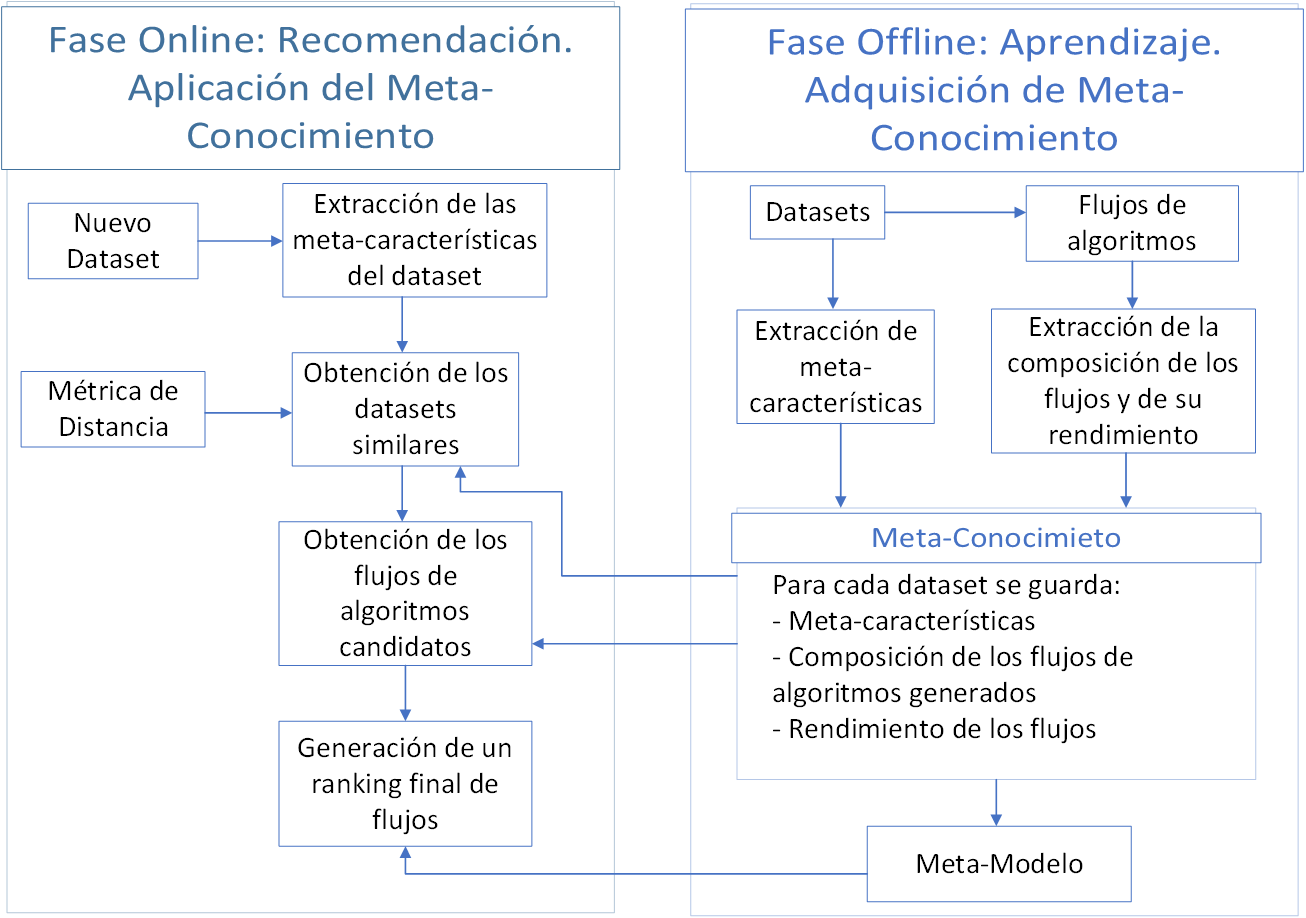
\includegraphics[scale=.4]{Figures/system.png}
	%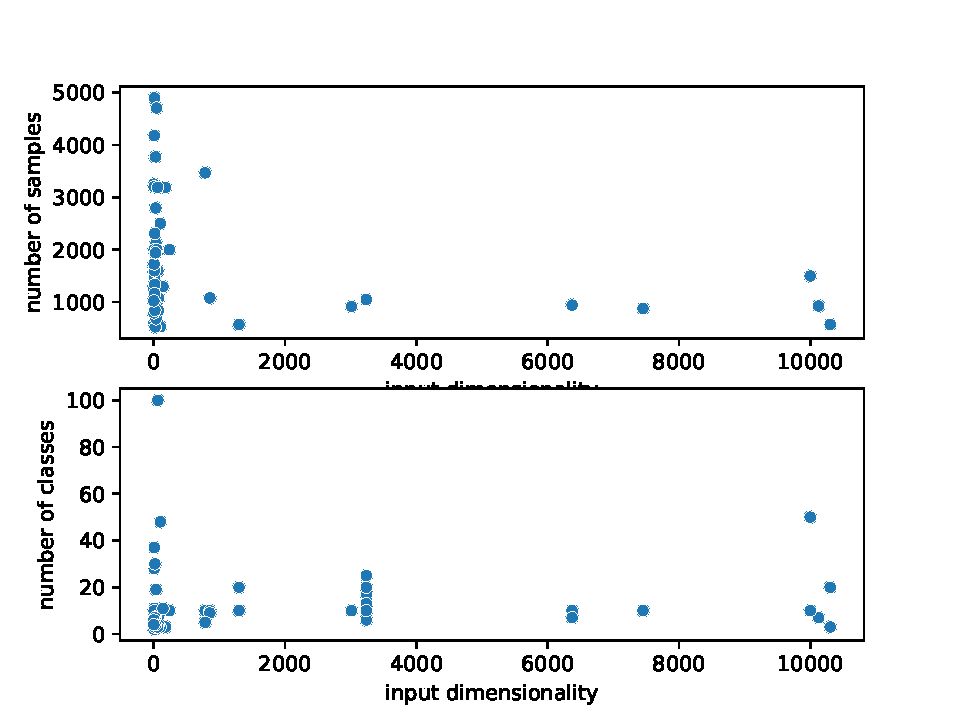
\includegraphics[scale=.60]{Figures/mtf scatterplot.pdf}
	\caption{Flujo de trabajo del enfoque de meta-learning propuesto.}
	\label{fig:system}
\end{figure}

La implementación de cada uno de estas fases es descrita en las siguientes secciones con más profundidad.

\subsection{Adquisición de meta-conocimiento}\label{sub:adquisicion}

%- Explicar cómo se realiza la adquisición de meta-conocimiento, con la extracción de meta-features y de información sobre los pipelines usados.
%- Explicar la importancia de las meta-features. Las meta-features extraídos de cada dataset deben ser suficientes para describir los aspectos principales del dataset, de tal manera que cada dataset pueda ser identificado mediante esta caracterización. Además, deben comprender las características necesarias para distinguir el rendimiento obtenido de diferentes algoritmos de aprendizaje cuando son aplicados a este dataset. 
%- Recordar un poco los distintos tipos de meta-features, describiéndolos un poco: simples, generales, estadísticas, teóricas de la información, basados en modelos, _landmarking_. Explicar que estos últimos dos no fueron implementados debido a su complejidad computacional.
%- Explicar la información que se extrajo sobre los pipelines: para cada dataset se extrajeron los mejores pipelines, explicar el formato en que fueron guardados (mediante el sampler de AutoGOAL), y el rendimiento que se obtuvo para cada uno de ellos.
%- Concluir mencionando que las meta-features y la estructura de los pipelines son usadas como características para el meta-modelo, y el rendimiento de los pipelines como etiquetas.

La adquisición de meta-conocimiento se realiza mediante la extracción de caracterizaciones de un conjunto de datasets, es decir, meta-características, y de información referente a un conjunto de algoritmos que deben ser probados en estos datasets. Entre los datos de los algoritmos extraídos se guarda información respecto a los hiperparámetros utilizados y al rendimiento alcanzado en cada una de las tareas para cada uno de los conjuntos de algoritmos usados.

\subsubsection{Características de los datasets}\label{subsub:metafeat}

Para extraer meta-características de una tarea de aprendizaje específica es necesario realizar un análisis de la información contenida en el dataset asociado a ella. Las meta-características, además de proveer información referente a los datos del dataset (relacionados con valores medios, desviación estándar, etc.), deben ser capaces de proporcionar conocimiento sobre la tarea que el dataset está representando.  Por lo tanto, las meta-características pueden ser concebidas como colecciones específicas de características de un dataset, las cuales proporcionan información relevante sobre la tarea que es necesario resolver mediante algoritmos de aprendizaje~\cite{castiello2005metadata}. La principal suposición es que el conocimiento codificado en las meta-características deben mostrar algún tipo de pista general (por ejemplo, relacionado a la complejidad de la tarea) que permita la solución de la tarea, en vez de limitarse a la información relacionada con el contenido del dataset (como la composición de sus datos). Con estas meta-características y una cantidad suficientemente grande de datasets es posible crear un meta-modelo que sea capaz de resolver una gran cantidad de tareas.

% Las meta-features extraídos de cada dataset deben ser suficientes para describir los aspectos principales del mismo, de tal manera que cada dataset pueda ser identificado mediante esta caracterización. Además, deben comprender las características necesarias para distinguir el rendimiento obtenido de diferentes algoritmos de aprendizaje cuando son aplicados. 

Como se mencionó anteriormente en el Capítulo \ref{chapter:review}, las meta-características se pueden separar en 5 categorías \cite{bradzil2009metalearning}:

\begin{itemize}
	\item \textit{Simples o generales:} Incluyen información general relacionada con un dataset determinado.
	\item \textit{Estadísticas:} describen las propiedades numéricas de la distribución de datos. %Pueden ser empleadas para tener en cuenta el número de propiedades, lo que le permite al meta-modelo discriminar el grado de correlación de los atributos numéricos y estimar su distribución.
	\item \textit{Teóricas de la información:} Son características del campo de teoría de la información, apropiadas particularmente para describir atributos categóricos, pero también pueden ajustar atributos continuos. %Semánticamente, describen la variedad y la redundancia de los atributos utilizados para representar las clases.
	\item \textit{Basados en modelos:} están caracterizadas por la extracción de información de un modelo de aprendizaje de predicción, generalmente, un árbol de decisión.
	\item \textit{Landmarking:} Usan el rendimiento de algoritmos de aprendizaje simples y rápidos para caracterizar los datasets.
\end{itemize}

Debido a la complejidad computacional requerida para el cálculo de los últimos dos tipos de meta-características, estos no fueron implementados. Sin embargo, se añadieron meta-características específicas de AutoGOAL, aprovechando la caracterización de los tipos semánticos de entrada y de salida que este sistema ofrece. Para evaluar el enfoque seguido se implementaron las siguientes meta-características, tomadas varios trabajos del estado del arte \cite{castiello2005metadata, fuerer2015efficient}.

\begin{itemize}
	\item \underline{\textsc{Simples}}: \begin{description}
		\item[Es supervisado:] determina si un problema es supervisado o no.
		\item[Tamaño de la muestra:] representa el número total \texttt{k} de instancias en el dataset (la cardinalidad del dataset).
		\item[Número de clases:] representa la cantidad de posibles de clases (etiquetas) presentes en el dataset que son posibles predecir.
		\item[Dimensionalidad de la entrada:] representa el número total \texttt{m} de atributos en el dataset.
		\item[Dimensionalidad de la salida:] representa el número total de valores de salida en el dataset.
		\item[Dimensionalidad del dataset:] representa la proporción entre el número de atributos y el número de observaciones del dataset, es decir, $dim_{dataset} = \dfrac{m}{k}$.
		\item[Cantidad de características categóricas:] cantidad de atributos del dataset que tienen valores categóricos.
		\item[Características categóricas:] determina si el dataset tiene atributos que tienen valores categóricos.
		\item[Cantidad de características numéricas:] cantidad de atributos del dataset que tienen valores numéricos.
		\item[Características numéricas:] determina si el dataset tiene atributos que tienen valores numéricos
		\item[Cantidad de valores faltantes:] cantidad de valores nulos del dataset.
	\end{description}
	\item \underline{\textsc{Estadísticos}}: \begin{description}
		\item[Desviación estándar:] estima la dispersión de la variable aleatoria $X = x_1, x_2, ..., x_k$ (las características del dataset) con respecto a su media $\overline{X} = \dfrac{1}{k}\sum^k_{i=1}x_i$. Es calculada como $std_X = \sqrt{\dfrac{1}{k}\sum^k_{i=1}(xi - \overline{X})^2}$
		\item[Coeficiente de variación:] evalúa la normalización de la desviación estándar de la variable aleatoria X con respecto a su valor medio: $VarCoeff_X =  \dfrac{std_x}{\overline{X}}$
		\item[Covarianza media:] la covarianza expresa la relación lineal entre dos variables aleatorias $X = x_1, ..., x_k$ y $Y = y_1, ..., y_k$ y está definida como: $Cov(X, Y) = \sum^k_{i=1} \dfrac{(x_i - \overline{X})(y_i - \overline{Y})}{k-1}$. La media de la covarianza entre todos los pares de atributos se usa como medida de covarianza de todo el dataset.
		\item[Coeficiente de correlación lineal:] análisis de correlación que intenta medir la fuerza de una relación entre dos variables aleatorias $X$ y $Y$. Puede ser estimado utilizando la siguiente fórmula: $\rho_{X, Y} = \dfrac{Cov(X, Y)}{\sqrt{std_X std_Y}}$. Como coeficiente de correlación lineal de todo el dataset se usa el promedio de las correlaciones entre todos los pares de atributos.
		\item[\textit{Skewness} (Oblicuidad):] mide la falta de simetría en la distribución de una variable aleatoria X, en este caso todo el dataset, para cada uno de los atributos. Está definido como $Skew_X = \dfrac{1}{std_X^3}\dfrac{\sum_{i=1}^{k}(x_i - \overline{X})^3}{k}$.  El resultado es un \texttt{array}, que es caracterizado devolviendo el valor medio, máximo, mínimo y la desviación estándar.
		\item[Curtosis:] mide el grado de concentración que presentan los valores de una variable alrededor de la zona central de la distribución de frecuencias, en este caso todo el dataset. Está definido como $Kurt_X = \dfrac{1}{std^4_X}\dfrac{\sum_{i=1}^{k}(x_i - \overline{X})^4}{k}$. El resultado es un \texttt{array}, que es caracterizado devolviendo el valor medio, máximo, mínimo y la desviación estándar.
		\item[PCA (\textit{Principal Component Analysis}, Análisis de los Componentes Principales):] es un método para transformar un determinado dataset en un nuevo dataset de dimensiones reducidas, para concentrar la información sobre las diferencias entre las instancias en un pequeño número de dimensiones. En PCA, el primer componente es un vector que representa la dirección de máxima varianza. Por estas razones se realiza el análisis de los componentes principales, y se retorna el \textit{skewnes} y la curtosis del primer vector.
	\end{description}
	\item \underline{\textsc{Teóricos de la Información}}: \begin{description}
		\item[Entropía normalizada de una clase:]  el valor de entropía $H(C)$ de una variable $C$ indica cuanta información es necesaria para especificar una clase (etiqueta). El valor de entropía $H(C)$ es evaluado usando la siguiente fórmula: $H(C) = \sum^n_{i=1}p_i log_2(p_i)$, donde $p_i$ es la probabilidad (frecuencia relativa) de ocurrencia de una clase $i$. Cuando suponemos que cada clase en un dataset tiene la misma probabilidad de aparecer, entonces el valor máximo teórico para la entropía de una clase es $log_2(n)$, por lo tanto, la entropía normalizada es calculada como: $H(C)_{norm} = \dfrac{H(C)}{log_2(n)}$
		\item[Entropía normalizada de un atributo:] el valor de entropía H(X) de un atributo X mide la información relacionada con los valores que X puede tener. La entropía normalizada de un atributo se calcula con la misma fórmula anterior: $H(X)_{norm} = \dfrac{H(X)}{log_2(n)}$. Para retornar un valor representado la entropía de todo el dataset se calcula la entropía de cada uno de sus atributos, y de estos valores es devuelto la media, el mínimo, el máximo y la desviación estándar.
		\item[Entropía conjunta:] mide la entropía total del sistema combinado de variables, es decir, de un par de variables (C, X), los cuales están representados por una variable de clase y uno de los M atributos de entrada discretizados respectivamente. Si $p_{ij}$ representa la probabilidad conjunta de observar el i-ésimo valor del atributo X y el j-ésimo valor de clase, la entropía conjunta está definida como: $H(C, X) = \sum_{i \in X, j \in C} p_{ij} log_2(p_{ij})$. Después de calcular la entropía para cada par clase-atributo, de estos valores se devuelve la media, el mínimo, el máximo y la desviación estándar.
		\item[Información mutua de clase y atributo:] mide la información común compartida entre dos variables aleatorias C y X. Si C y X representan una variable de clase y un atributo de entrada respectivamente, entonces esta meta-característica mide la información contenida por el atributo X sobre una variable de clase y describe la reducción de incertidumbre para C debido al conocimiento de X. La información mutua de clase y atributo es evaluada usando la fórmula: $MI(C, X) = H(C) + H(X) - H(C, X)$. Como medida para describir todo el dataset, se calcula la entropía para cada par clase-atributo, de estos valores se devuelve la media, el mínimo, el máximo y la desviación estándar.
		\item[Número equivalente de atributos:] en lo referente a las tareas de clasificación, la información requerida para especificar una clase es $H(C)$ y ningún sistema de clasificación puede ser completamente existoso a no ser que se proporcione  $H(C)$ pedazos de información. Esta meta-característica proporciona información sobre la complejidad de un problema, específicamente el número de atributos de un dataset determinado que es adecuado para resolver la tarea de clasificación. Es evaluada mediante la proporción entre la entropía de clase $H(C)$ y el promedio de la información mutua $\overline{MI(C, X)}$ como: $EN_{attr} = \dfrac{H(C)}{\overline{MI(C, X}}$
		\item[Relación de la señal de ruido:]  mide la cantidad de información irrelevante contenida en un dataset. Si se considera $\overline{MI(C, X)}$ como una medida de información útil de una clase y $\overline{H(X)} - \overline{MI(C, X)}$ como una medida de información no útil, la meta-característica puede ser evaluado como: $NS.ratio = \dfrac{\overline{H(X)} - \overline{MI(C, X}}{\overline{MI(C, X)}}$
	\end{description}
	\item \textsc{\underline{Específicos de AutoGOAL}}: \begin{description}
		\item[Tipo semántico de la entrada y de la salida:] AutoGOAL representa diferentes tipos de datos semánticos que recogen el concepto de compatibilidad de tipos. Estos tipos se representan como una jerarquía de clases en la cual la herencia determina la relación de compatibilidad. Los tipos de datos tienen una interpretación semántica más allá de su estructura computacional subyacente. Por ejemplo, una lista de valores puede representar un vector de valores discretos o un vector de categorías, dependiendo de la interpretación más adecuada para un problema determinado. En su implementación actual, AutoGOAL define 23 tipos semánticos de datos, incluyendo varios para datos de lenguaje natural, como \texttt{Token} o \texttt{Stem}.
	\end{description}
\end{itemize}

Es posible la caracterización de estas meta-características por más de un aspecto, además de la categorización por tipos estudiada. Por ejemplo, el tipo de tarea de ML que describe. Algunas meta-características están restringidas a tareas específicas, como la clasificación, mientras otras pueden aplicarse de manera más genérica a tareas supervisadas, como problemas de regresión. En las tareas supervisadas y de clasificación, se necesita un atributo destino para evaluar las meta-características, que no es necesario para las meta-características de cualquier tipo. Las meta-características clasificadas como ``Cualquiera'' son las más generales y también se pueden aplicar a tareas no supervisadas como \textit{clustering} y problemas semi-supervisados. 

Además de la tarea de destino, las meta-características pueden ser descritas por el tipo de datos de los argumentos admitidos. Algunas meta-características solo pueden manejar atributos numéricos, mientras que otras están restringidas a categorizar atributos. Un tercer grupo admite ambos tipos de atributos, sin hacer ninguna distinción entre ellos. Aunque el dominio de una función generalmente se define en términos de un conjunto de valores o un tipo de datos específico, como entero, real y de cadena, la distinción entre numérico y categórico es suficiente para el análisis de meta-características~\cite{Rivolli2018TowardsRE}.  

En la Tabla~\ref{tab:metafeat} se muestran las meta-características utilizadas junto con sus características en dependencia del tipo de meta-característica, el tipo de tarea de aprendizaje automático destino y el dominio de entrada de los atributos usados.

\begin{center}
	\begin{longtable}{l|c|c|c}
		\caption{Caracterización del conjunto de meta-características.} 		\label{tab:metafeat} \\
		\hline
		\textbf{Meta-Característica} & \textbf{Tipo} & \textbf{Tarea} & \textbf{Dominio} \\
		\hline \hline
		\endfirsthead
		\multicolumn{4}{c}%
		{\tablename\ \thetable\ -- \textit{Continuación de la página anterior}} \\
		\hline
		\textbf{Meta-Característica} & \textbf{Tipo} & \textbf{Tarea} & \textbf{Dominio} \\
		\hline \hline
		\endhead
		\hline \multicolumn{4}{r}{\textit{Continúa en la siguiente página}} \\
		\endfoot
		\hline
		\endlastfoot
		Supervisado & Simple & Cualquiera & Ambos \\ 
		Tamaño de la muestra & Simple & Cualquiera & Ambos \\ 
		Número de clases & Simple & Clasificación & Ambos \\ 
		Dimensionalidad de la entrada & Simple & Cualquiera & Ambos \\
		Dimensionalidad de la salida & Simple & Cualquiera & Ambos \\ 
		Dimensionalidad del dataset & Simple & Cualquiera & Ambos \\ 
		Cantidad Características categóricas & Simple & Cualquiera & Categórico \\ 
		Características categóricas & Simple & Cualquiera & Categórico \\
		Cantidad de características numéricas & Simple & Cualquiera & Numérico \\ 
		Características numéricas & Simple & Cualquiera & Numérico \\
		Cantidad de valores faltantes & Simple & Cualquiera & Ambos \\ \hline
		Desviación estándar & Estadística & Cualquiera & Numérico \\
		Coeficiente de variación & Estadística & Cualquiera & Numérico \\ 
		Covarianza media & Estadística & Cualquiera & Numérico \\ 
		Coeficiente de correlación lineal & Estadística & Cualquiera & Numérico \\ 
		\textit{Skewness} & Estadística & Cualquiera & Numérico \\
		Curtosis & Estadística & Cualquiera & Numérico \\ 
		PCA & Estadística & Cualquiera & Numérico \\ \hline 
		Entropía normalizada de una clase & Teórica de la Info. & Clasificación & Ambos \\ 
		Entropía normalizada de un atributo & Teórica de la Info. & Cualquiera & Ambos \\
		Entropía conjunta & Teórica de la Info. & Clasificación & Ambos \\ 
		Información mutua de clase y atributo & Teórica de la Info. & Clasificación & Ambos \\ 
		Número equivalente de atributos & Teórica de la Info. & Clasificación & Ambos \\ 
		Relación de la señal de ruido & Teórica de la Info. & Clasificación & Ambos \\ \hline
		Tipo semántico de la entrada & AutoGOAL & Cualquiera & Ambos \\
		Tipo semántico de la entrada & AutoGOAL & Cualquiera & Ambos \\ \hline
	\end{longtable}
\end{center}

\subsubsection{Características de las soluciones}\label{subsub:soluciones}

Además de las meta-características, se extrajo información relacionada con las soluciones de las tareas, que fueron utilizadas como características para el meta-modelo. En la fase de adquisición de conocimiento, la solución de las tareas deben ser generadas. El enfoque de meta-learning implementado no intenta simplemente determinar un buen algoritmo con sus hiperparámetros como solución, sino un flujo de algoritmos, lo que complica la generación de estos. Un flujo $p = <a^1, ..., a^2>$  puede ser visto como un caso especial de algoritmo que aplica cada algoritmo $a^i$ de forma secuencial a la salida del algoritmo anterior en la secuencia. Formalmente, se puede ver como la composición de los algoritmos correspondientes, es decir, $p(x) = a^n(a^{n-1}(...a^1(x)...))$.

Para la generación de los flujos de algoritmos se utilizó AutoGOAL. En cada uno de los datasets se ejecutó AutoGOAL y se guardaron las arquitecturas generadas junto con su rendimiento. El formato en el que se guardaron fue dependiente de la estructura en la que AutoGOAL procesa los flujos. Los algoritmos se ponen primero secuencialmente, luego existe una palabra clave \texttt{End} para representar el final de estos. Después, se ponen los hiperparámetros de los algoritmos de la forma  `\texttt{\{algoritmo\}\_\{hiperparámetro\}}' para identificarlos. En el algoritmo~\ref{alg:flows} se muestra un ejemplo del formato JSON en el que son guardados los flujos. Además de las estructuras de los flujos de algoritmos, se guardó el modelo probabilístico que siguió AutoGOAL para la formación de dicho flujo.

\begin{algorithm}
\begin{lstlisting}[language=json,firstnumber=1]
{
  "FeatureAgglomeration": [1],
  "KNeighborsClassifier": [1],
  "End": [1],
  "FeatureAgglomeration_n_clusters": [3],
  "FeatureAgglomeration_affinity": [0],
  "FeatureAgglomeration_compute_full_tree": [0],
  "FeatureAgglomeration_linkage": [0],
  "KNeighborsClassifier_n_neighbors": [5],
  "KNeighborsClassifier_weights": [0],
  "KNeighborsClassifier_algorithm": [2],
  "KNeighborsClassifier_leaf_size": [23],
  "KNeighborsClassifier_p": [3],
  "KNeighborsClassifier_metric": [0]}
\end{lstlisting}
\caption{Ejemplo de como se almacenan los flujos generados por AutoGOAL}
\label{alg:flows}
\end{algorithm}

En una de las estrategias seguidas, se implementa un meta-modelo que usa las meta-características de los datasets de entrenamiento y la representación de los flujos de algoritmos generados como características y el rendimiento de estos flujos como etiquetas. Esta información es utilizada para su entrenamiento.

Una vez adquirido el meta-conocimiento se procede a la aplicación del mismo.

\subsection{Aplicación de meta-conocimiento}\label{sub:aplicacion}

%- Explicar qué se hace en esta fase de aplicación de meta-conocimiento, su objetivo es la obtención de una lista de pipelines prometedores para un dataset determinado.  Esto se realiza analizando los datasets similares y recomendando los pipelines que tuvieron un buen rendimiento en dichos datasets. 
%- Explicar un poco el resto de la sección mencionando las 2 estrategias llevadas a cabo.

En un sistema de meta-learning la aplicación de meta-conocimiento puede ser utilizado para ayudar a seleccionar un conjunto de algoritmos de aprendizaje de máquinas que obtengan un buen rendimiento en una tarea determinada. Una vez obtenidos los meta-datos necesarios, el objetivo de esta fase es la obtención de una lista de flujos de algoritmos prometedores para un dataset determinado. Esto se realiza analizando los datasets similares a un nuevo dataset y recomendando los flujos que tuvieron un buen rendimiento en estos conjuntos de datos seleccionados. 

La selección de algoritmos fue realizada mediante un enfoque de ranking, en el que para un nuevo dataset se seleccionan los \texttt{k} mejores flujos de algoritmos. Para esto se implementaron varias estrategias, que son descritas a continuación.


\subsubsection{Estrategia de Vecinos Cercanos}\label{subsub:nn}

%- Explicar de forma general cómo funciona la estrategia de nearest neighbors, mencionar que es de las estrategias más usadas. Consiste en extraer las _k_ instancias más similares a un dataset nuevo, y formar un ranking de recomendación seleccionando los _n_ pipelines de mejor rendimiento de los datasets seleccionados para el nuevo dataset.
%- Explicar que está compuesta por varios pasos, en el primer paso, dado un dataset nuevo, se computan sus meta-features y se selecciona un conjunto de _k_ instancias en el conjunto de entrenamiento que son similares al dataset actual. Generalmente la similitud está basada en una métrica de distancia, hablar de cuáles fueron las implementadas.
%- Explicar el segundo paso: se seleccionan los _n_ mejores pipelines de los _k_ mejores datasets y se genera un ranking para el nuevo dataset, explicar cómo se genera ese ranking.

La primera estrategia, de \textit{Nearest Neighbors} o Vecinos Más Cercanos, consiste en extraer los flujos candidatos para un dataset determinado en dependencia de las características de los \texttt{n} datasets más similares a él. Se extraen los \texttt{m} flujos de algoritmos que hayan tenido mejor rendimiento en cada uno de los \texttt{n} datasets, y estos flujos son combinados para formar un nuevo ranking para el nuevo dataset. Este enfoque puede ser dividido en dos pasos: la búsqueda de los vecinos cercanos y la generación de un ranking.

En el primer paso, dado un dataset nuevo, se calculan sus meta-características con el objetivo de construir un vector de características. Luego, se selecciona un conjunto de \texttt{n} instancias (vecinos cercanos) en el conjunto de entrenamiento que son similares al nuevo dataset. Esta similitud está basada en una medida de distancia (por ejemplo, la distancia euclidiana), que es aplicada entre los vectores de características de los datasets de entrenamiento y el nuevo dataset. La solución seguida soporta cualquier función de similitud, para comprobar el funcionamiento del sistema el siguiente conjunto de medidas fueron implementadas:

\begin{itemize}
%	\item similitud coseno: es una medida de similitud existente entre dos vectores en un espacio que posee un producto interior con el que se evalúa el valor del coseno comprendido entre ellos. $$cos(\theta) = \dfrac{A \multiply B}{||A||||B||}$$.
	\item Distancia de Manhattan o L1: la distancia $d_1$ entre dos vectores A y B en un espacio n-dimensional es la suma de las diferencias absolutas entre cada una de los componentes de los vectores. Más formalmente, $d_1(A, B) = {||A - B||}_1 = \sum^n_{i=1} |a_i - b_i|$, donde $A = a_1, a_2, ..., a_n$ y $B = b_1, b_2, ..., b_n$
	\item Distancia Euclidiana o L2: es la distancia ``ordinaria'' entre dos puntos de un espacio euclidiano, la cual se deduce a partir del teorema de Pitágoras. La distancia entre dos vectores $A = a_1, a_2, ..., a_n$ y $B = b_1, b_2, ..., b_n$ en un espacio n-dimensional se define como: $d_2(A, B)=\sqrt{(a_1 - b_1)^2 + (a_2 - b_2)^2 + ... + (a_n - b_n)^2}$
\end{itemize}

En el segundo paso, se obtienen los rankings de los \texttt{m} flujos de algoritmos con mejor rendimiento para cada uno de los \texttt{n} datasets similares seleccionados. Luego, estos rankings son combinados para formar un ranking de los \texttt{k} mejores flujos de algoritmos para el nuevo dataset. El nuevo ranking es generado en dependencia del rendimiento de los \texttt{m} flujos de algoritmos en sus respectivos dataset. Por ejemplo, si se seleccionan los $2$ datasets más cercanos, $d_1$ y $d_2$ y para cada uno de estos datasets se obtienen $2$ flujos: $p^1_1$ y $p^1_2$ para $d_1$ y $p^2_1$ y $p^2_2$ para $d_2$ con los siguientes resultados: $p^1_1 = 0.98$, $p^1_2 = 0.90$ , $p^2_1 = 0.99$, $p^2_2 = 0.97$, estos resultados son combinados obteniendo el ranking final para el nuevo dataset: $p^2_1$, $p^1_1$, $p^2_2$ y $p^1_2$. En el Algoritmo~\ref{alg:nn.proc} se muestra el pseudocódigo con un resumen de los pasos seguidos para la obtención del ranking final de flujos de algoritmos.

\begin{algorithm}
	\begin{algorithmic}
		 \State $\vartriangleright$ Primer Paso
		 \State $meta\_caracteristicas \gets \textbf{preprocesar\_meta\_carcateristicas}(dataset)$
		
		 \State $similar\_datasets \gets \textbf{similar\_datasets}(meta\_caracteristicas, metrica\_distancia,\text{ }\texttt{n})$  \\\\
		 
		 $\vartriangleright$ Segundo Paso 
		 
		 \State $flujos, rendimientos \gets \textbf{mejores\_flujos}(similar\_datasets,\text{ }\texttt{m}) $
		 
		 \State $ranking \gets \textbf{ordenar\_flujos\_por\_rendimiento}(flujos,\text{ }rendimientos,\text{ } \texttt{k})$ \\
		 \Return ranking
	\end{algorithmic}
	\caption{Procedimiento para obtener el ranking de mejores flujos en la estrategia de Vecinos Cercanos.}
	\label{alg:nn.proc}
\end{algorithm}

Una de las desventajas de este enfoque es la necesidad de especificar y determinar los mejores valores para la cantidad de datasets similares seleccionados \texttt{n} y la cantidad de flujos de algoritmos seleccionados \texttt{m}. Además, este enfoque no tiene en cuenta la magnitud de la medida de similitud entre los dos datasets. Por ejemplo, en el caso de que un dataset determinado sea muy similar a uno de los dataset de entrenamiento puede ser mejor seleccionar los \texttt{m} mejores flujos de ese dataset nada más. Por otro lado, si el dataset es bastante diferente a todos los datasets del conjunto de entrenamiento debe ser mejor seleccionar el mejor flujo en los \texttt{n} datasets más similares. Por estas razones fue implementada otra estrategia de generación de rankings. 

El otro método para la generación de rankings consiste en un mecanismo ponderado entre dos factores: la distancia entre el nuevo dataset y los datasets del conjunto de entrenamiento, y el valor del resultado de rendimiento de los flujos de algoritmos en los dataset similares. Aunque con esta solución no es necesario especificar los valores de \texttt{n} y \texttt{m}, existen infinitas maneras de combinar estos dos factores. La estrategia seguida para su combinación fue una de las más directas: la división entre el resultado de rendimiento de un flujo de algoritmos en un dataset similar y el valor de distancia entre los dataset. De esta forma, los datasets que tengan menor distancia entre sí y los flujos que tengan un mejor rendimiento obtendrán un mayor resultado. Los resultados de esta división son los utilizados para generar el ranking de los flujos candidatos para la nueva tarea.

Este último enfoque tiene una desventaja, y es que los pares dataset-flujo guardados en la base de conocimiento puede ser un número grande. Por lo tanto, para una mayor eficiencia del algoritmo se utiliza la información referente al tamaño del ranking final. Si se tiene que el resultado final va a ser un ranking de, por ejemplo, 15 flujos, entonces nunca va a ser necesario analizar más de los 15 flujos con mejor rendimiento en cada uno de los datasets. El mismo razonamiento se puede aplicar con la cantidad de datasets, es poco probable que sea útil analizar más allá de los 15 datasets más similares, sin embargo, esta última heurística no funciona siempre. Falla en el caso de  
de que los flujos de algoritmos en los primeros datasets tengan un rendimiento bajo. %que haya poca diferencia en la similitud de los 16 primeros datasets y además los flujos de algoritmos probados tengan una puntuación baja, y luego el dataset 16 tenga un flujo con un alto rendimiento, en cuyo caso, será mejor elegir el último dataset. Por estos razonamientos, esta última heurística no fue implementada. Para cada uno de los datasets se analizan los 15 mejores flujos de algoritmos de todos los datasets. 
Por estos razonamientos, solo la primera heurística fue implementada y para cada uno de los datasets de la base de conocimiento se analizan solamente los 15 mejores de flujos.

La estrategia de generación de ranking más usada en la literatura~\cite{fuerer2015efficient, sun2014MetaLearningAT, bradzil2009metalearning} se basa en \textit{average ranking} o ranking promedio~\cite{bradzil2009metalearning}. 
%Sea $R_{i,j}$ el ranking del algoritmo $T_{j}$, $j=1,...,t$ en el dataset $i$, donde $t$ es el número de algoritmos, el ranking promedio de cada algoritmo $T_{j}$ está definido como: $\overline{R_{j}} = \sum^{k}_{i=1}R_{i,j} / k$, donde $k$ es el número de datasets similares. Es decir, el ranking promedio de un algoritmo no es más que el promedio del ranking obtenido en cada uno de los datasets seleccionados.
El ranking promedio de un algoritmo es el promedio del ranking obtenido por dicho algoritmo en cada uno de los datasets seleccionados. El ranking final es calculado ordenando los rankings promedio de todos los algoritmos. Una de las razones por la que esta estrategia no fue usada, es que este método de agregación de rankings requiere la evaluación de cada flujo de algoritmos en todos los datasets, por lo que la agregación de un nuevo dataset en la base de conocimiento requiere la evaluación de todos los flujos de algoritmos anteriores en el dataset. Usualmente, se implementa mediante la selección de un conjunto predefinido de flujos de algoritmos, por lo que no existe mucha variedad en los flujos utilizados para la inicialización de los procesos de optimización. La estrategia de generación de ranking seguida por la implementación del método de vecinos cercanos proporciona una forma fácil de agregar nuevos datasets a la base de conocimiento usada, y una mayor variedad en los flujos de algoritmos utilizados.

\subsubsection{Estrategia utilizando un Meta-Modelo}\label{subsub:ranker}

%- Explicar también de forma general cómo funciona esta estrategia. En esta estrategia se usa un algoritmo de ranking para predecir el rendimiento de un par dataset-pipeline sin necesidad de ejecutar dicho pipeline. Midiendo la similitud de los dataset con un nuevo dataset se extraen un conjunto de pipelines recomendados, y estos algoritmos son presentados junto con el dataset nuevo al meta-modelo, obteniendo un ranking de pipelines recomendados.
%- Esta estrategia también funciona en 2 fases: en la primera fase se computan los meta-features del nuevo y se seleccionan los datasets similares y los pipelines candidatos de una manera similar a la del método anterior.
%- Se diferencian en la 2da fase, en donde se usa un meta-modelo (xgbranker) que usa una estrategia de ranking para predecir qué tan relevante son los pipelines candidatos para el nuevo dataset.
%- Poner cómo son preprocesados los pipelines para ser usados en el meta-modelo.

La segunda estrategia utiliza un meta-modelo para predecir el rendimiento de un flujo de algoritmos en un determinado dataset sin necesidad de ejecutar dicho flujo. Al igual que en la estrategia anterior dado un nuevo dataset se extraen los flujos más similares a él, y se obtiene un conjunto de flujos candidatos. Estos flujos son presentados al meta-modelo junto con el nuevo dataset para obtener un ranking de los algoritmos candidatos. Esta estrategia también funciona en dos pasos.

En el primer paso se computan las meta-características del nuevo dataset, y se sigue un método parecido a la estrategia anterior para obtener los dataset similares. La similitud se mide con una métrica de distancia entre los vectores de características de los datasets que se quieren comparar. Para la solución del sistema cualquier función de similitud puede ser utilizada, se implementaron y se probaron las mismas funciones que en la estrategia anterior: distancia L1 y distancia L2.

Los datasets similares son usados para determinar los flujos de algoritmos que son presentados al meta-modelo. En vez de presentar todos los flujos obtenidos del conjunto de entrenamiento al meta-modelo, por cuestiones de eficiencia, se seleccionan solo los más prometedores, que son los que tienen mayor rendimiento en los datasets similares. Para determinar cuántos datasets y flujos de algoritmos extraer se utiliza la información referente al tamaño del ranking final que se quiere obtener. Si, por ejemplo, se quiere obtener un ranking de 15 flujos, entonces se seleccionan los 15 datasets más similares al dataset en cuestión y de estos datasets se extraen los 15 flujos de mejor rendimiento. 

Los flujos de algoritmos obtenidos necesitan ser pre-procesados para ser presentados al meta-modelo. Con el objetivo de representar los flujos de una forma compacta, se eligió representar la topología de un flujo como una secuencia de números. Cada algoritmo del flujo está representado como un número único que lo identifica. Por lo tanto, se genera una secuencia de números para representar cada flujo, donde el orden de los números determina el orden de aplicación de los algoritmos que componen el flujo.

Los algoritmos contenidos en los flujos de algoritmos que genera AutoGOAL tienen los hiperparámetros optimizados, pero esta información no es utilizada para el entrenamiento del meta-modelo. La dificultad de ese enfoque es que aumentaría el tamaño del espacio de características considerablemente. El problema de meta-learning cuenta con relativamente pocas instancias de entrenamiento (datasets) y una gran cantidad de características haría que fuese difícil para el meta-modelo generalizar.

Se utilizaron solo los algoritmos sin sus hiperparámetros para que el meta-modelo sepa cuáles algoritmos tienen un buen rendimiento, de manera general, en un dataset determinado. Sin embargo, para cada secuencia de algoritmos en un dataset se pueden recuperar los algoritmos con sus hiperparámetros, ya que estos están guardados en la base de conocimiento. En el caso de que exista una secuencia igual de algoritmos en un mismo dataset se puede considerar el flujo con mejor resultado de rendimiento. Al final, cuando el meta-modelo genera un ranking, la secuencia de números es descodificada y los hiperparámetros de los algoritmos que componen el flujo de algoritmos son retornados. Por lo tanto, en el ranking final se recuperan los hiperparámetros de los algoritmos seleccionados.

En la segunda fase de la estrategia, los flujos de algoritmos candidatos pre-procesados son concatenados con el vector de características del nuevo dataset, formando los meta-datos, y son presentados al meta-modelo. Como resultado, el meta-modelo retorna un ranking basado en el rendimiento esperado de cada uno de los flujos en el dataset. Se retorna una lista con los \texttt{k} mejores flujos y, como se mencionó anteriormente, estos flujos son post-procesados para obtener los hiperparámetros con los que fueron utilizados en su dataset original. En el Algoritmo~\ref{alg:ranker.proc} se resumen todos los pasos seguidos para la generación del ranking final.
 
% For the training of our meta-learner, we used XGBoost [7]. More specifically, we used the XGBRanker model with the pairwise rank- ing objective function and shallow trees of 150 estimators. This was done since our problem is in its essence a ranking problem, and previous work [4] has shown that XBGoost is highly suitable for producing ranked lists. Additionally, we used the following hyper- parameters settings: learning rate of 0.1, max depth of 8 and 150 estimators. We set the number of pipelines returned by RankML to k = 10. The algorithm’s parameters were empirically set using the leave-one-out approach.

\begin{algorithm}[H]
	\begin{algorithmic}
		\State $\vartriangleright$ Primer Paso
		\State $meta\_caracteristicas \gets \textbf{preprocesar\_meta\_carcateristicas}(dataset)$
		
		\State $similar\_datasets \gets \textbf{similar\_datasets}(meta\_caracteristicas,\text{ }metrica\_distancia,\text{ }\texttt{k})$  
		
		\State $flujos, rendimientos \gets \textbf{mejores\_flujos}(similar\_datasets,\text{ } \texttt{k})$
		
		\State $flujos\_codificados \gets \textbf{codificar\_flujos}(flujos)$ \\\\
		
		$\vartriangleright$ Segundo Paso
		
		\State $caracteristicas \gets \textbf{unir\_caracteristicas}(meta\_caracteristicas,\text{ }flujos\_codificados)$
		
		\State $y \gets model.\textbf{predict}(caracteristicas)$ 
		
		\State $mejores\_flujos \gets \textbf{ordenar\_flujos}(flujos\_codificados,\text{ }y,\text{ }\texttt{k})$
		
		\State $ranking \gets \textbf{decodificar\_flujos}(mejores\_flujos)$ \\
		
		\Return ranking
	\end{algorithmic}
	\caption{Procedimiento para obtener el ranking de mejores flujos en la estrategia utilizando un meta-modelo.}
	\label{alg:ranker.proc}
\end{algorithm}


Como meta-modelo, se utilizó el modelo XGBRanker de la biblioteca XGBoost~\cite{xgboost} de Python. Este meta-modelo fue elegido porque el problema seleccionado es en esencia un problema de ranking, y trabajo previo ha demostrado que XGBoost es altamente recomendado para producir listas rankeadas~\cite{rankml}. Además, XGBoost ha sido usado con anterioridad en problemas de meta-learning para la selección de algoritmos~\cite{rankml, atomic}.

XGBoost es una biblioteca de aprendizaje automático ampliamente utilizada, que utiliza técnicas de aumento de gradiente para construir gradualmente un mejor modelo durante la fase de entrenamiento mediante la combinación de múltiples modelos débiles. Los modelos débiles son modelos simples, En XGBoost se generan calculando el descenso del gradiente usando una función objetivo. El modelo construido así se utiliza luego para la predicción en una futura fase de inferencia. \textit{Learning to rank} (LTR) o Aprender a rankear es una de esas funciones objetivos.

LTR es una clase de técnicas que aplica aprendizaje de máquinas supervisado para resolver problemas de ranking. La principal diferencia entre LTR y ML supervisado tradicional es que ML resuelve un problema de predicción (clasificación o regresión) en una sola instancia en el tiempo, mientras que LTR resuelve un problema de ranking retornando una lista de elementos. El objetivo de LTR es proponer una ordenación óptima para esos elementos. La aplicación más común de LTR es el ranking en los motores de búsqueda, pero es útil en cualquier lugar donde necesite producir una lista rankeada de elementos.

XGBoost utiliza el algoritmo de clasificación LambdaMART~\cite{burges2010from} para árboles potenciados (o \textit{boosted trees}), que utiliza el enfoque de ranking por pares (\textit{pairwise ranking}). Ranking por pares es uno de los enfoques más comunes en LTR, donde se elige un par de instancias y se predice el orden de esas dos. Al repetir este procedimiento para cada par se encuentra el orden final. En XGBoost se elige un par de instancias para cada ejemplo de entrenamiento durante el aprendizaje, y el gradiente se calcula en función del orden relativo entre ellos.

%Adicionalmente, se usaron las configuraciones de hiperparámetros siguientes:
%\begin{itemize}
%	\texttt{n\_estimators = 110}: Es el número de los gradient boosted trees. Equivalente al número de rondas de boosting. (boosting rounds)
%	\item \texttt{max\_depth = 6}: La profundidad máxima de los árboles para los base learners
%	\item \texttt{learning\_rate = 0.1}: boosting learning rate
%	\item \texttt{objective = `rank:pairwise'}: especifica la tarea de aprendizaje y el correspondiente objetivo de aprendizaje.
%	\item \texttt{booster = `gbtree'}: especifica cuál booster usar: gbtree, gblinear, o dart
%	\item \texttt{tree\_method = `hist'}: especifica cuál método de árbol usar
%	\item \texttt{subsample = 0.75}: proporción de la submuestra de la instancia de entrenamiento.
%	\item \texttt{random\_state = 43}: Número de semilla aleatoria.
%	\item \texttt{predictor = `cpu\_predictor'}: Obliga a XGBoost a usar un predictor en específico, las opciones disponibles son: \texttt{`cpu\_predictor'} y \texttt{`gpu\_predictor'}.
%\end{itemize}

\section{Implementación en AutoGOAL}\label{sec:autogoal_imp}

%- Hablaría de varias estrategias para la utilización del conjunto inicial obtenido por el método de meta-learning. 
%- Hablar un poco de la estrategia de optimización de AutoGOAL, para describir la estrategia usada para la inicialización del proceso de búsqueda.
%- Hablar un poco de detalles de implementación, como el conocimiento guardado fue convertido en las estructuras que usa AutoGOAL para su búsqueda.

La estrategia llevada a cabo hasta ahora puede funcionar como un sistema de recomendación de flujos de algoritmos independiente, o puede servir como un paso preliminar para otras soluciones más complejas computacionalmente, como las soluciones presentadas al problema de CASH en el Capítulo~\ref{chapter:review}. Sin embargo, a pesar de que mediante meta-learning puede sugerir rápidamente algunas inicializaciones de los algoritmos de ML que probablemente tengan buenos resultados, no es posible obtener información detallada sobre qué tan buen rendimiento tendrá en un dataset nuevo. En contraste, los algoritmos de optimización utilizados en herramientas de AutoML son lentos al buscar en grandes espacios de hiperparámetros, pero son capaces de obtener información más detallada sobre el rendimiento de los algoritmos de ML en un nuevo dataset~\cite{fuerer2015efficient}. Es por esto que el enfoque de meta-learning propuesto es complementario al proceso de optimización, usando el ranking de configuraciones elegidas para inicializar un proceso de optimización.

Como herramienta de AutoML complementaria a esta solución se eligió el sistema de AutoGOAL~\cite{autogoal}, que ha sido diseñado por el grupo de investigación de Inteligencia Artificial de la Facultad de Matemáticas y Computación. AutoGOAL se destaca por su capacidad de abordar una gran variedad de problemas, combinando técnicas y algoritmos de diferentes bibliotecas, incluidos clasificadores lineales, herramientas de procesamiento de lenguaje natural y redes neuronales. Esta característica lo hace ideal como herramienta adicional para la solución del problema propuesto.

Para comprender cómo la técnica de meta-learning propuesta fue añadida a AutoGOAL primero es necesario entender como este sistema de AutoML representa el espacio de búsqueda para resolver el problema de CASH. El espacio de búsqueda en AutoGOAL se representa como un grafo $G_A$ dirigido y acíclico (DAG), donde cada nodo representa un algoritmo. Las aristas se definen entre algoritmos con tipos de entrada/salida compatibles. Los espacios de configuraciones de hiperparámetros de cada uno de los algoritmos corresponden a gramáticas libres del contexto definidas para cada nodo. Los hiperparámetros con valores continuos, discretos, categóricos o booleanos generan producciones que producen un valor aleatorio de una distribución adecuada. AutoGOAL aprovecha esta estructura de grafo definida para un problema específico y genera automáticamente una gramática general a partir del DAG correspondiente.

Dada un problema específico con tipos $T^*_{in}$ , $T^*_{out}$ de entrada y salida respectivamente, una solución consiste en un flujo $p =<a^1, ..., a^n >$ tal que el tipo $T^*_{in}$ sea compatible con el tipo $T^p_{in}$ y el tipo $T^p_{out}$ sea compatible con el tipo $T^*_{out}$. Considerando el grafo construido anteriormente $G_A$, se añaden dos nodos ficticios, el nodo Entrada y el nodo Salida, que representan los tipos de entrada y de salida respectivamente. Los algoritmos con tipos de entrada compatible con el primero tendrán una arista desde el mismo, mientras que los compatibles con la salida presentarán una arista hacia el segundo. En este grafo cualquier camino que comience en el nodo Entrada y termine en el nodo Salida representa un flujo que resuelve dicho problema.

En AutoGOAL sobre el grafo de algoritmos $G_A$ de un problema específico se realiza un proceso de optimización para descubrir los mejores flujos válidos mediante generación aleatoria. Este proceso de optimización se basa en evolución gramatical probabilística para gramáticas libres del contexto~\cite{pge2015}, y consiste en un ciclo de generación y evaluación utilizando una gramática construida a partir de $G_A$, dirigida por un modelo probabilístico $\sigma$.

Para generar los flujos de algoritmos, primero se debe considerar que, por construcción, cada nodo pertenece a un camino válido. Por tanto, realizando un recorrido aleatorio comenzando por el nodo Entrada, si no se repiten nodos y toda arista tiene probabilidad de cruzarse mayor que 0, entonces se garantiza que este recorrido termina en el nodo Salida. A cada algoritmo $a_i$ en $G_A$ se le asigna un peso (no normalizado) $w_i$, que se utiliza para seleccionar un vecino aleatorio durante la generación de un camino en $G_A$ siguiendo una distribución multinomial Bernoulli. La Figura~\ref{fig:autogoal} muestra una representación visual del proceso descrito anteriormente.

\begin{figure}[H]
	\centering
	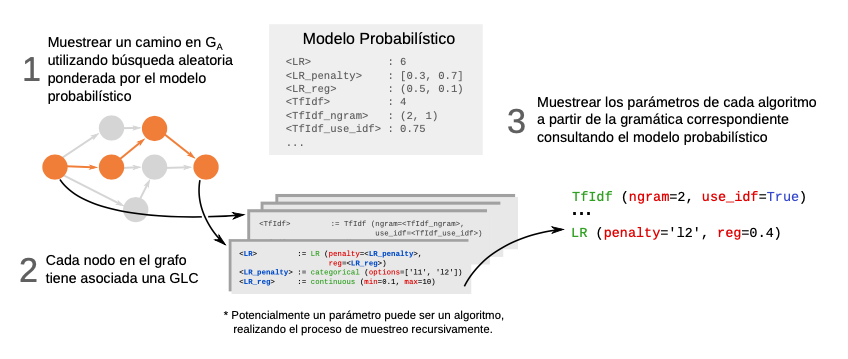
\includegraphics[scale=.5]{Figures/autogoal.png}
	\caption{Representación visual del proceso de creación y muestreo del
		espacio de búsqueda.}
	\label{fig:autogoal}
\end{figure}

El modelo $\sigma$ se inicializa con valores neutrales para cada distribución (pesos uniformes para distribución categórica, media centrada y máxima varianza para distribuciones continuas). El proceso de optimización consiste en un ciclo de generación y evaluación. Primeramente, se generan \texttt{n} flujos siguiendo el modelo de muestreo. Utilizando una función de evaluación $\Phi(p)$ (dada por el usuario para el problema a resolver) se evalúan los flujos y se seleccionan los $k < n$ mejores. El valor del mejor flujo del ciclo es comparado con el mejor global y actualizado en consecuencia. Tomando los valores de muestra de los hiperparámetros generados, se construye un modelo probabilístico marginal $\sigma^*$. Luego, el modelo $\sigma^*$ y el modelo marginal $\sigma$ son mezclados usando un factor de interpolación $\alpha \in [0, 1]$, ofreciendo un balance entre exploración y explotación. Este ciclo se repite hasta que se llegue a un límite de tiempo de ejecución, una cantidad determinada de iteraciones, o hasta que no se encuentre mejora. Por cada iteración el modelo $\sigma$ converge lentamente a un modelo que maximiza la probabilidad de producir los mejores flujos. 

La estrategia seguida para la inicialización del proceso de optimización de AutoGOAL es la modificación del modelo probabilístico $\sigma$. Después de obtener la lista de flujos de algoritmos recomendados en la fase de meta-learning, se extraen los modelos probabilísticos asociados a estos flujos. Estos modelos son guardados en la fase inicial de meta-learning, de obtención de meta-conocimiento, cuando se generan los flujos con AutoGOAL. Luego, se crea un modelo inicial $\sigma^*$, que es el resultado de la mezcla de los modelos probabilísticos de los flujos recomendados. En las primeras iteraciones se usa el modelo $\sigma$ con valores neutrales para cada distribución, generando flujos aleatorios, para lograr una mayor exploración y luego este modelo es mezclado con el modelo $\sigma^*$, que contiene las inicializaciones que son resultado de la fase de meta-learning. Al igual que en el proceso de optimización de AutoGOAL tradicional, se utiliza un factor de interpolación $\alpha \in [0, 1]$, ofreciendo un balance entre exploración y explotación. El resto del proceso de optimización de AutoGOAL ocurre normalmente.


% !TeX spellcheck = es_ES
\chapter{Resultados Experimentales}\label{chapter:results}

% - Hacer un overview del capítulo
El objetivo de este capítulo es evaluar los métodos propuestos de meta-learning en la tarea de la creación de un ranking de algoritmos y en su utilización como inicialización de un intenso proceso de optimización. El estudio realizado se enfoca solo en el rendimiento del algoritmo de meta-learning en los datasets de clasificación. Para ser capaces de sacar conclusiones estadísticamente significativas, se eligieron 305 datasets, en dependencia de los recursos computacionales y el tiempo disponible. En este capítulo se explica el método seguido para la obtención de dichos datasets, la distribución de sus características y el procedimiento seguido para la formación de los conjuntos de entrenamiento y de prueba utilizados en la experimentación (Sección~\ref{sec:datasets}). Luego, se describe la metodología seguida para la generación de los flujos de algoritmos que son usados como experiencia pasada por los métodos de meta-learning propuestos (Sección \ref{sec:flujos}). Primero se describe brevemente las configuraciones utilizadas en los modelos implementados (Sección~\ref{sec:comparacion}), y después 
%se realiza una evaluación de la precisión del ranking para evaluar la eficiencia de los modelos en cuanto a la creación de rankings de algoritmos (Sección \ref{subsec:ranking}). Posteriormente, 
se exponen los resultados obtenidos al añadir las configuraciones recomendadas por los métodos propuestos en la inicialización de la optimización de AutoGOAL, comparándolas con la versión de AutoGOAL que no tiene meta-learning (Sección~\ref{subsec:resultados}). Se evalúan varios aspectos, como la cantidad de flujos inválidos generados durante la optimización y los resultados finales obtenidos para cada una de las estrategias. Por último, se presenta una discusión sobre los resultados obtenidos y se mencionan algunas limitaciones del método propuesto (Sección~\ref{sec:discusion}).


\section{Datasets}\label{sec:datasets}

%- Hablar un poco de openml, que fue usado para extraer los datasets
%
%- Hablar de cuales fueron los datasets seleccionados y cómo fueron seleccionados
%
%- Características de los datasets seleccionados
%
%- Hablar de cómo fueron divididos los datasets para la experimentación

Para los experimentos realizados se extrajeron datasets de clasificación de OpenML \cite{vanschoren2014openml}. OpenML es una plataforma de código abierto desarrollada con el objetivo de permitir a los investigadores compartir sus datasets, implementaciones y experimentos de una forma tal que ellas puedan ser fácilmente encontradas y reusadas por otros. OpenML tiene alrededor de 19000 datasets disponibles para descargar y ofrece una API Web\footnote{\url{http://www.openml.org}} a través de la cual pueden ser enviados nuevos recursos y resultados. OpenML-Python \cite{feurer2019openmlpy} es una integración al ecosistema popular de Python ML\footnote{\url{https://github.blog/2019-01-24-the-state-of-the-octoverse-machine-learning/}}, que elimina la complejidad del acceso a la API Web proporcionando un fácil acceso en Python a todos los datos de OpenML y automatizando el intercambio de nuevos experimentos. Los datasets seleccionados fueron extraídos utilizando esta API.
 
 Para obtener un conjunto representativo de datasets se consideraron todos los que tenían más de 300  y menos de 500 000 instancias con más de 2 atributos y menos de 300 atributos, terminando en un total de 305 datasets. Estos datasets son muy diversos con respecto a su número de instancias, número de características, y número de clases. Características sobre su distribución pueden verse en la Figura \ref{fig:datasets}
 
 \begin{figure}[H]
\centering
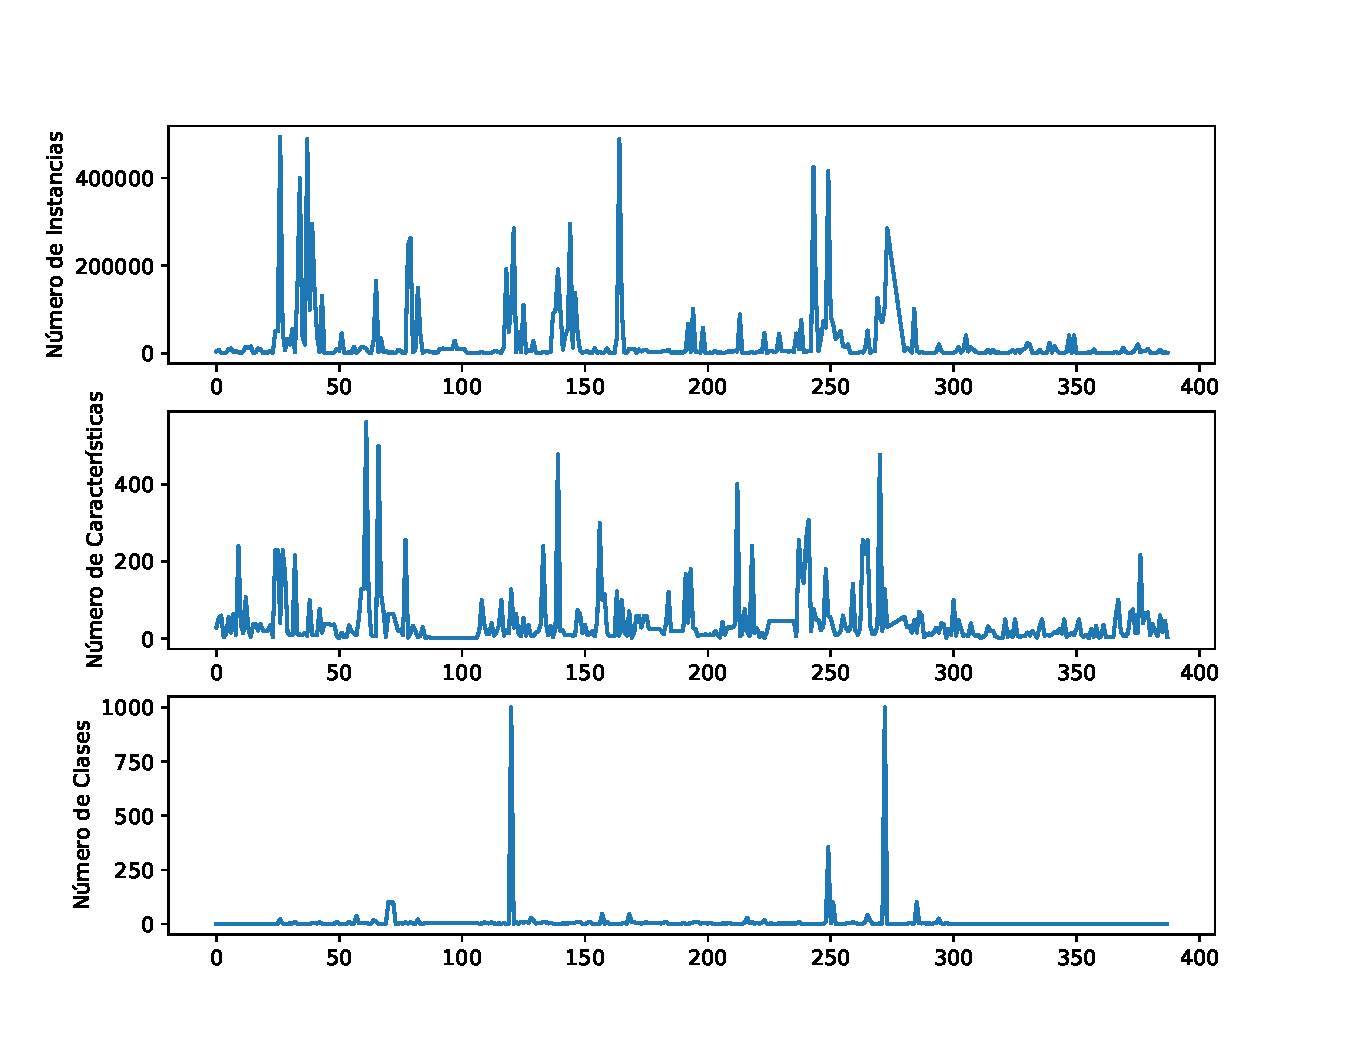
\includegraphics[scale=.75]{Figures/mtf-lineplot.pdf}
%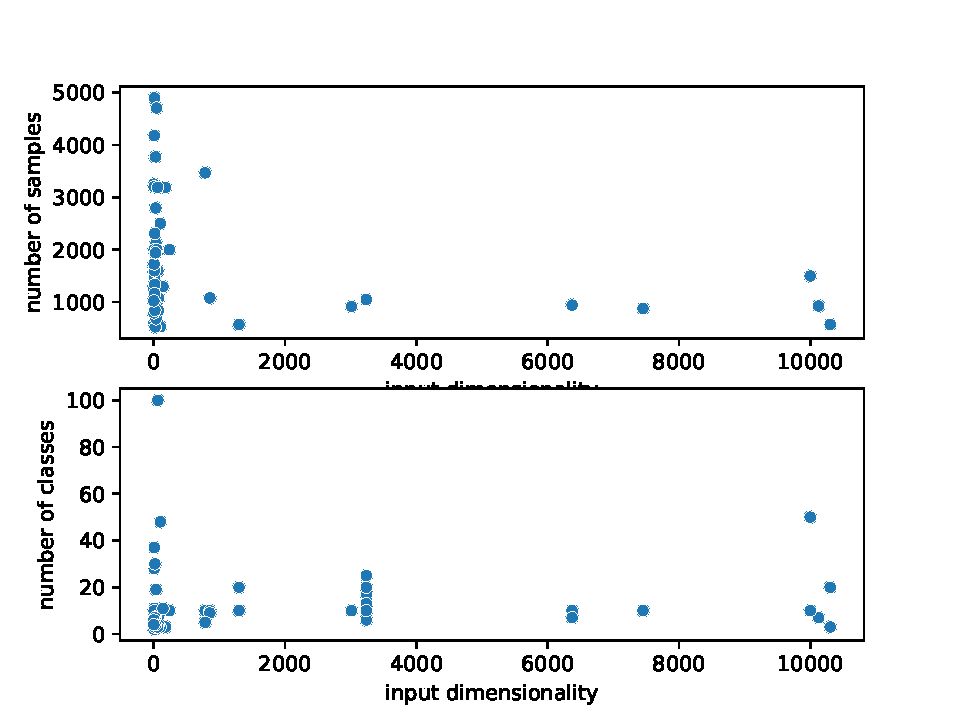
\includegraphics[scale=.60]{Figures/mtf scatterplot.pdf}
\caption{Características de los datasets en cuanto al número de instancias, número de características y número de clases.}
\label{fig:datasets}
\end{figure}
 
 
 Para la evaluación de la propuesta realizada se separaron los 305 datasets en dos conjuntos: $D_{train}$ y $D_{test}$, donde el primero representa el $75\%$ del total de datasets y el segundo el $25\%$. $D_{train}$ fue utilizado en el entrenamiento de las estrategias seleccionadas y $D_{test}$ en la prueba de las mismas. %El conjunto de datasets de entrenamiento $D_{train}$ fue a su vez dividido en 2, usándose el segundo para la evaluación de los modelos implementados. De $D_{train}$ se usó el $75\%$ para el entrenamiento y el $25\%$ como validación, es decir, para obtener resultados parciales en cuanto al rendimiento del método implementado. 
 En los resultados mostrados en el resto de este capítulo, se usa todo el conjunto de datasets $D_{train}$ para el entrenamiento de los modelos obtenidos con las distintas estrategias implementadas y se exponen los resultados obtenidos en $D_{test}$.

 
 \section{Generación de Flujos}\label{sec:flujos}
 
% - Introducir la sección hablando de los tipos de algoritmos por los que está compuesto AutoGOAL (las bibliotecas que se usó, etc)
% - Hablar de cómo fue el proceso de entrenamiento de AutoGOAL para la extracción de solución, hablando de la configuración usada en AutoGOAL para la búsqueda de flujos.
% - Terminar hablando del tiempo total de entrenamiento, la cantidad total de flujos de algoritmos generados y el promedio de flujos generados por dataset.

Todos los flujos de algoritmos usados durante el entrenamiento y evaluación de la propuesta implementada fueron generadas usando AutoGOAL. Los flujos generados con AutoGOAL consisten en algoritmos prensentes en varias bibliotecas de Python, entre las que se encuentran: Sklearn~\cite{scikit-learn}, Pytorch~\cite{paszke2019pytorch}, Keras~\cite{chollet2015keras}, NLTK~\cite{bird2009natural} y Gensim~\cite{khosrovian2008gensim}.

AutoGOAL se ejecutó en cada uno de los 305 datasets seleccionados y se almacenaron todas las arquitecturas generadas junto con los resultados obtenidos. Para cada uno de los datasets, AutoGOAL se configuró para que realizara la búsqueda de flujos durante 1 hora, teniendo un total de 5 minutos para la evaluación de un flujo de algoritmos. De esta forma, se excluyeron flujos muy complejos y se garantizó la evaluación de al menos 12 flujos por dataset. Esta generación de flujos duró un total de 305 horas y se generaron en promedio 640.28 flujos de algoritmos por dataset, y en total se obtuvieron 248 430  flujos. 

Estos flujos generados son utilizados como base de conocimiento para el método propuesto. Como se explica en la Sección~\ref{subsub:soluciones}, los flujos almacenados son utilizados para recomendar configuraciones iniciales en el proceso de optimización en dependencia de los datasets considerados similares al dataset que se quiere evaluar.

\section{Comparación de diferentes estrategias}\label{sec:comparacion}

%- Hacer un pequeño resumen de las configuraciones de las estrategias y variantes implementadas
%
%- Hacer un resumen del resto de la sección.

Los datasets y los flujos de algoritmos extraídos fueron utilizados con las diferentes estrategias de meta-learning implementadas:

\begin{description}
	\item[Estrategia Vecinos Cercanos Simple:] El método de vecinos cercanos, tal como está descrita en la Sección~\ref{subsub:nn}, fue probado utilizando la distancia L2 estándar. El ranking final generado para un nuevo dataset es de 15 flujos. En esta versión se utilizó la estrategia simple, en la que se seleccionan \texttt{n} datasets más cercanos y de ellos los \texttt{m} flujos de algoritmos que hayan obtenido un mejor rendimiento, luego el ranking es formado seleccionando a los 15 mejores flujos de algoritmos. Para la evaluación de esta estrategia se utilizó \texttt{m = 15} y \texttt{n = 15}.
	\item[Estrategia Vecinos Cercanos Ponderado:] El método de vecinos cercanos se vuelve a evaluar, pero utiliza la otra estrategia explicada en la Sección~\ref{subsub:nn}. Esta estrategia consiste en un mecanismo ponderado entre dos factores: la distancia entre el nuevo dataset y los datasets en el conjunto de entrenamiento, y el valor del resultado del rendimiento de los flujos de algoritmos en los datasets similares. Estos factores son divididos, y el valor obtenido es el usado para generar el nuevo ranking. Al igual que en la estrategia anterior, se utiliza la distancia L2 estándar y se genera un ranking final de 15 flujos para una tarea nueva.
	\item[Estrategia usando XGBRanker:] En esta estrategia, explicada en la sección~\ref{subsub:ranker}, se utilizó como meta-modelo XGBRanker de la biblioteca XGBoost para generar los rankings de una nueva tarea. Se usaron las siguientes configuraciones de hiperparámetros: 	
	\begin{itemize}
		\item \texttt{objective = `rank:pairwise'}: especifica la tarea de aprendizaje y el correspondiente objetivo de aprendizaje. En este caso, se eligió \textit{rank} porque es una tarea de \textit{ranking} y \textit{pairwise} porque utiliza el enfoque de ranking por pares (en inglés, \textit{pairwise ranking}).
		\item \texttt{n\_estimators = 150}: Es el número de los árboles con gradientes aumentados (\textit{gradient boosted trees}) utilizados en el algoritmo de ranking de XGBoost explicado en la Sección~\ref{subsub:ranker}.
		\item \texttt{tree\_method = `hist'}: especifica el algoritmo de construcción de árboles usados en XGBoost~\cite{xgboost}. XGBoost dispone de 4 métodos: \texttt{exact}, \texttt{approx}, \texttt{hist}, \texttt{gpu\_hist}. El algoritmo elegido fue \texttt{hist}, que es el algoritmo más rápido, ya que es optimizado mediante un algoritmo \textit{greedy}.
		\item \texttt{max\_depth = 10}: La profundidad máxima de los árboles utilizados como modelos básicos. El aumento de este valor hace al modelo más complejo y hace que sea más probable que ocurra sobreajuste.
		\item \texttt{learning\_rate = 0.1}: especifica la tasa de aprendizaje.
		\item \texttt{subsample = 0.95}: proporción de la submuestra tomada de las instancias de entrenamiento. El valor 0.95 indica que XGBoost muestrearía al azar el 95\% del conjunto de entrenamiento para prevenir el sobreajuste. Esto se realiza una vez en cada iteración del algoritmo.
%		\item \texttt{colsamplebytree = 0.9}: es la proporción de submuestra de las columnas al construir cada árbol. El submuestreo ocurre una vez para cada árbol construido.
		% 		\item \texttt{random_state = 43}: Número de semilla aleatoria usado en los procesos aleatorios.
 		\item \texttt{predictor = `cpu\_predictor'}: especifica el tipo de algoritmo de predicción a usar. Los algoritmos disponibles proporcionan los mismos resultados, pero permiten el uso de la GPU o la CPU. La configuración usada fue la CPU.
	\end{itemize}
\end{description}


%\subsection{Evaluación de la Precisión del Ranking}\label{subsec:ranking}
%
%%- Explicar que se midió la precisión del ranking obtenido en las diferentes estrategias con diferentes medidas
%%
%%- Explicar cada una de las métricas de evaluación usadas
%%
%%- Explicar cómo se realizó esta experimentación
%%
%%- Poner resultados.
%
%Uno de los indicadores de eficiencia de la propuesta desarrollada es la precisión del ranking obtenida en cada una de las propuestas llevadas a cabo. Para evaluar la eficacia de los modelos se compararon los rankings predichos para un determinado dataset con sus correspondientes etiquetas de ranking. Dado dos conjuntos de rankings de tamaño \texttt{k}: $T = [T_1, T_2, ..., T_k]$ y $P = [P_1, P_2, ..., P_k]$, los cuales son los valores de relevancia objetivos y predecidos respectivamente, las siguientes métricas de evaluación de ranking y funciones fueron usadas en los experimentos realizados:
%
%\begin{description}
%	\item[Coeficiente de Correlación de Rango de Spearman]o \textit{Spearman’s Rank Correlation Coefficient} (SRCC). SRCC evalúa que tan  bien puede ser descrita la relación entre el ranking verdadero y el predicho. Está definido como: $$\rho_{srccc} = 1 - \dfrac{6\sum^k_{i=1}(T_i - P_i)^2}{k(k^2-1)}$$
%	
%	\item[Coeficiente de Rango Ponderado]o \textit{Weighted Rank Correlation} (WRC). La métrica WRC le da más peso a los mejores candidatos. Ha sido usado en varios trabajos de meta-learning~\cite{sun2014MetaLearningAT, soares2004learning, costa2005weighted}. Está definido como: $$\rho_{wrc} = 1 - \dfrac{1-\sum^k_{i=1} (T_i - P_i)^2(2k - T_i - P_i + 2) }{k ^4+k^3-k^2-k}$$
%	
%	\item[Ganancia Acumulada Descontada Normalizada]o \textit{Normalized Discounted Cumulative Gain} (NDCG). Es una métrica de efectividad usada a menudo en motores de búsqueda usando una escala de relevancia calificada de elementos en una lista de resultados. Para entender la métrica NDGC es necesario entender primero las métricas de Ganancia Acumulada (\textit{Cumulative Gain}, CG) y Ganancia Acumulada Descontada (\textit{Discounted Cumulative Gain}, DCG).
%	
%	
%	CG es la suma de los valores de relevancia predecidas de todos los resultados en la lista resultante. Matemáticamente, $$CG = \sum^k_{i=1}P_i$$
%	
%	El problema de CG es que no tiene en cuenta el ranking del conjunto resultante cuando determina la utilidad del conjunto. En otras palabras, si se reordenase las puntuaciones de relevancias predichas no obtendríamos un mejor conocimiento de un conjunto resultante, ya que CG no cambiará.
%	
%	Para superar esto se introduce DCG. DCG penaliza los resultados con un mayor valor de relevancia que aparecen más abajo en la búsqueda, reduciendo la relevancia predicha en dependencia de la posición del resultado. Formalmente, $$DCG = \sum^k_{i=1} \dfrac{2^{P_i} - 1}{log_2(i + 1)}$$
%	
%	Un problema surge con DCG cuando se quiere comparar el resultado de diferentes rankings porque la lista de resultados puede variar en longitud. Por lo tanto, normalizando la ganancia acumulada en cada posición se llega a NDCG. Esto se realiza ordenando los valores objetivos por su relevancia relativa, produciendo el máximo valor posible en la posición \texttt{p}. Esta última medida se denomina Ganancia Acumulada Descontada Ideal (\textit{Ideal Discounted Cumulative Gain}, IDCG), que se calcula como: $$\sum^k_{i=1} \dfrac{2^{T_i} - 1}{log_2(i+1)}, $$ donde k es la cantidad de resultados relevantes.
%	Luego, NDCG se calcula como: $$NDCG = \frac{DCG_p}{IDCG}$$
%\end{description}
%
%La siguiente figura muestra los resultados obtenidos en cada una de las estrategias explicadas en la Sección~\ref{sec:comparacion}.
%
%[hablar un poco de los que se ve en las gráficas]
%
%%Por otro lado, también se obtiene un buen rendimiento al usar el sistema de recomendación de meta-learning para predecir flujos de algoritmos por sí solos. Es decir, sin añadir un extenso proceso de optimización posteriormente. Estas afirmaciones se pueden demostrar mediante los buenos resultados obtenidos para la predicción de rankings realizados.
%

\subsection{Resultados Experimentales}\label{subsec:resultados}

%- Explicar cómo se realizaron los experimentos.
%
%- Hablar de los diferentes aspectos evaluados (flujos inválidos, mejor resultado, iteraciones para el mejor resultado...).
%
%- Exponer los resultados.

%La eficacia del método implementado no se basa solo en qué tan bueno es para la creación de rankings  de flujos de algoritmos basados en experiencias pasadas. 

Para la evaluación de las estrategias de meta-learning implementadas es importante conocer los resultados obtenidos al incorporarse a un sistema de AutoML. Cómo el ranking de configuraciones elegidas son usadas para inicializar el proceso de optimización, y qué resultados este proceso puede obtener al usar el conocimiento previo adquirido mediante meta-learning. En esta sección se discuten las experimentaciones realizadas para evaluar estos aspectos.

Para la realización de los experimentos se ejecutó la búsqueda de algoritmos de AutoGOAL con y sin meta-learning, probando los métodos de meta-learning mencionados anteriormente: vecinos cercanos con la estrategia simple, vecinos cercanos utilizando mecanismos ponderados y utilizando un modelo de XGBoost, XGBRanker. Para estudiar su rendimiento bajo una estricta restricción de tiempo, y además, debido a limitaciones de los recursos computacionales utilizados, se limitó la búsqueda para cada ejecución a 30 minutos. Igualmente, el tiempo de ejecución de un solo modelo se limitó a la sexta parte de este tiempo (5 minutos). Las evaluaciones realizadas en esta sección muestran los resultados obtenidos en los datasets de prueba, utilizando los datasets de entrenamiento para entrenar los métodos implementados. % Cada estrategia se ejecutó 3 veces, y los resultados mostrados son el promedio de estas ejecuciones. 

Uno de los aspectos a analizar es la cantidad de flujos de algoritmos inválidos generados durante el proceso de optimización. Los flujos inválidos se encuentran en dos casos: cuando se excede el tiempo de espera predefinido por el investigador, o cuando ocurren errores de tiempo de ejecución impredecibles, como errores de falta de memoria provocados por una combinación inviable de hiperparámetros. Estas circunstancias a menudo son difíciles de predecir de antemano y no se pueden tener en cuenta en las gramáticas de AutoGOAL. Sin embargo, mediante la información adquirida con meta-learning se espera que la cantidad de flujos inválidos disminuya, ya que se utiliza conocimiento adquirido de problemas similares que usan flujos de algoritmos válidos.

En la Figura \ref{fig:failedpipelines}, se muestran los resultados obtenidos respecto a la proporción de flujos inválidos generados usando cada una de las estrategias desarrolladas, incluyendo la versión de AutoGOAL que no utiliza la inicialización de meta-learning. Como se puede observar, con las estrategias de meta-learning de Vecinos Cercanos Simple y XGBRanker se obtiene en promedio menor cantidad de flujos inválidos generados, mientras que en la estrategia de Vecinos Cercanos Ponderado se generan más flujos inválidos por dataset en promedio, por lo que no se puede determinar si la mejora obtenida con meta-learning es estadísticamente significativa. La generación de flujos inválidos es un factor que depende de muchos factores, y se cree que para demostrar la mejora en este aspecto es necesario una mayor experimentación.

\begin{figure}[H]
\centering
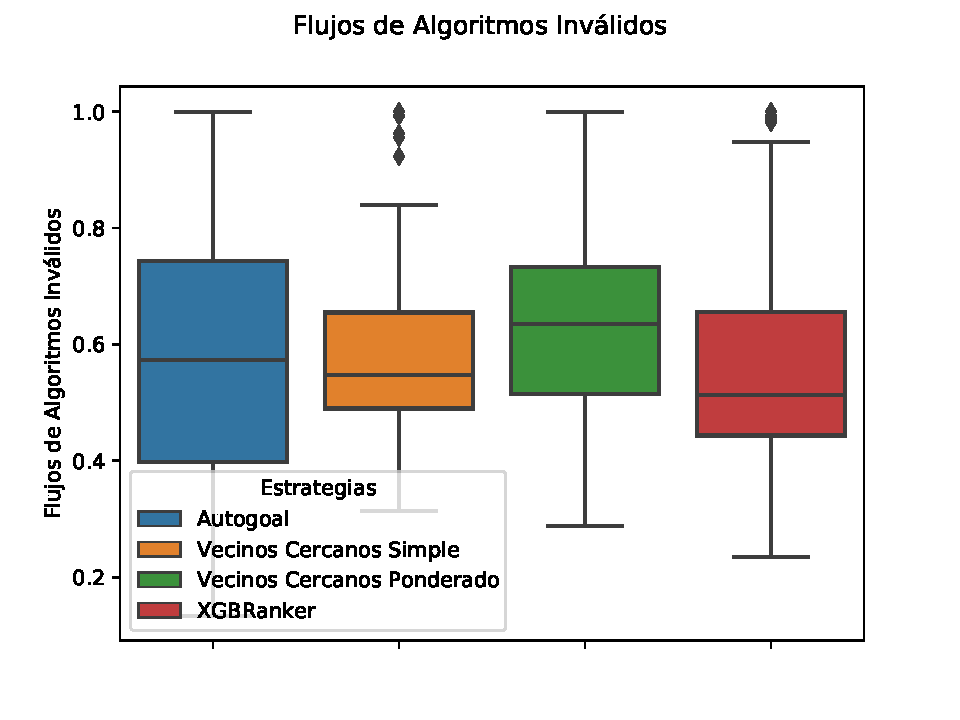
\includegraphics[scale=.8]{Figures/failed-pipelines.pdf}
\caption{Proporción de flujos de algoritmos inválidos generados en cada uno datasets usando las diferentes estrategias.}
\label{fig:failedpipelines}
\end{figure}

%Otro de los aspectos que puede ser interesante evaluar son las iteraciones necesarias para la obtención del mejor resultado. La Figura \ref{fig:maxidx} muestra los resultados obtenidos a través de las iteraciones en las diferentes versiones evaluadas. Se puede observar que las dos estrategias de vecinos cercanos obtuvieron el mejor resultado en menos iteraciones que AutoGOAL sin meta-learning. Sin embargo, la estrategia de XGBRanker no obtuvo el mismo resultado. % El resultado más sorprendente es que meta-learning produjo mejoras drásticas a partir de la primera configuración que seleccionó y que se prolongó hasta el final del experimento. La mejora fue más pronunciada al principio y, con el tiempo, AutoGOAL sin meta-learning también encontró buenas soluciones, lo que le permitió alcanzar los mismos resultados obtenidos en las versiones que usan meta-learning en algunos datasets (mejorando así su clasificación general).
%
%\begin{figure}[H]
%\centering
%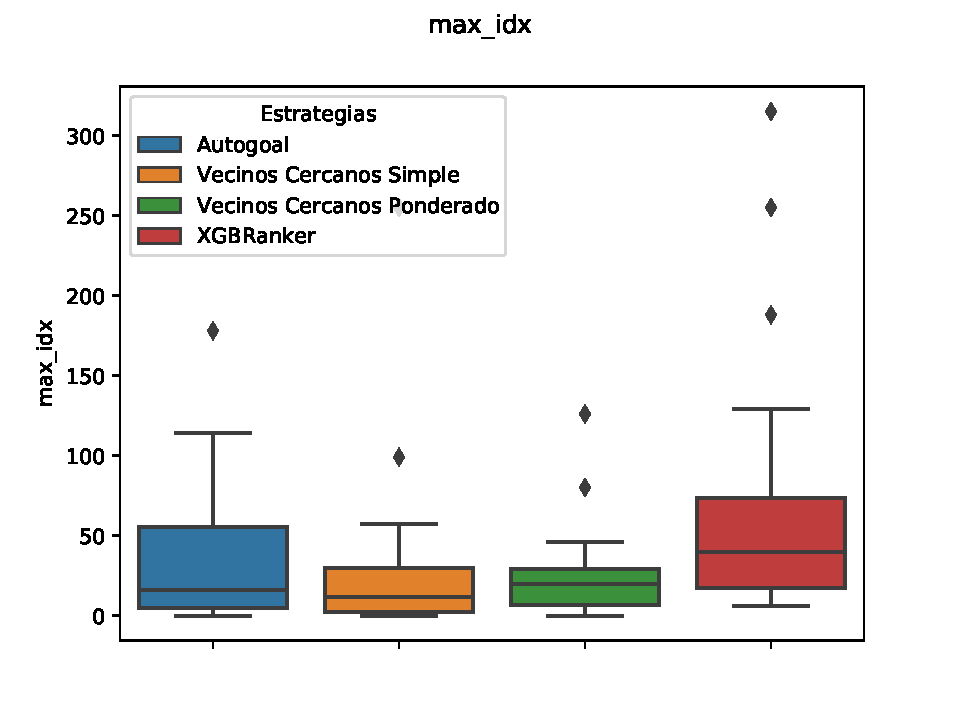
\includegraphics[scale=.60]{Figures/max idx.pdf}
%\label{fig:maxidx}
%\caption{Cantidad de iteraciones necesarias para la obtención del mejor resultado promedio en cada uno datasets usando las diferentes estrategias.}
%\end{figure}

Otro de los aspectos interesantes para evaluar es el comportamiento de las soluciones obtenidas a través de las distintas iteraciones de AutoGOAL. La Figura~\ref{fig:performance} muestra la media y el intervalo de confianza del 95\% de los resultados de rendimiento obtenidos en las primeras 200 iteraciones en las diferentes estrategias evaluadas. Se puede observar como, a partir de determinado punto (cuando se terminan las iteraciones iniciales que generan resultados aleatorios) las soluciones que utilizan meta-learning alcanzaron mejoras drásticas a partir de la primera configuración que se seleccionó. La mejora fue más pronunciada al principio y, con el tiempo, AutoGOAL sin meta-learning también encontró buenas soluciones, lo que le permitió alcanzar los mismos resultados obtenidos en las versiones que usan meta-learning en algunos datasets (mejorando así su resultado final). 

%En la mayor parte del tiempo estos resultados se mantienen, por lo que las soluciones de meta-learning superan a las soluciones obtenidas mediante AutoGOAL sin el uso de meta-learning.

\begin{figure}[H]
\centering
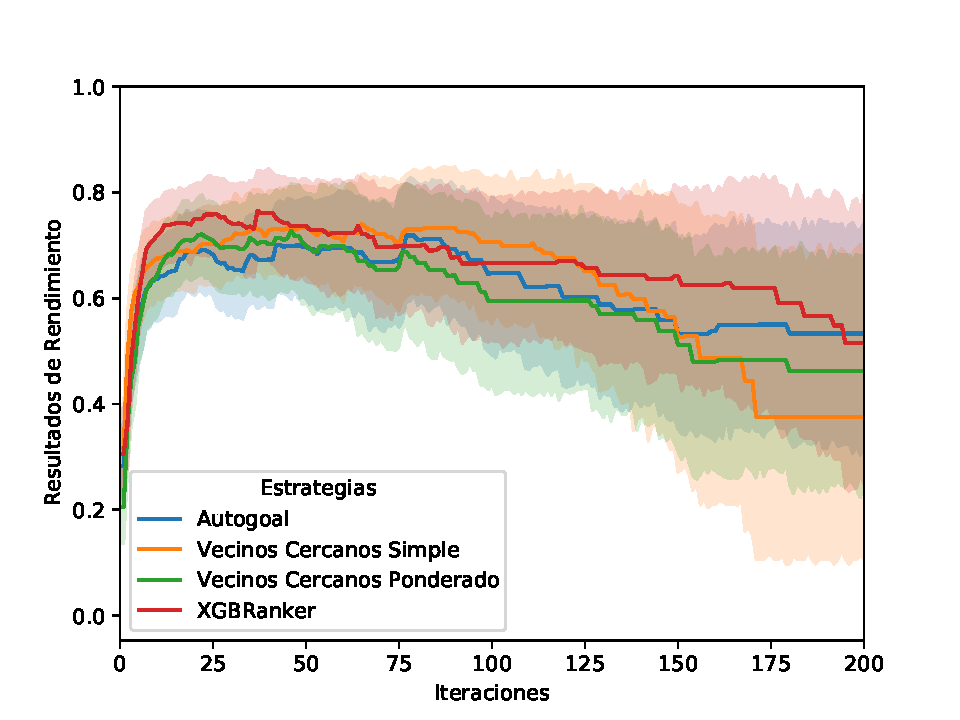
\includegraphics[scale=.8]{Figures/performance.pdf}
\caption{Resultados de rendimiento obtenidos en los datasets de prueba en las primeras 200 iteraciones, se muestra la media y el intervalo de confianza del 95\%.}
\label{fig:performance}
\end{figure}

En la Figura \ref{fig:bestfn} se muestra el mejor resultado final obtenido en la búsqueda de los flujos de algoritmos en cada uno de los datasets de prueba para las diferentes estrategias. Como se puede apreciar, se obtienen mejores resultados finales en cada uno de las estrategias seguidas con respecto a AutoGOAL sin meta-learning. La diferencia entre la estrategia de vecinos cercanos simple no es tan pronunciada con respecto a  la versión que no usa meta-learning, y esto se cree que se debe a que, a pesar de que mediante esta estrategia se obtienen los valores óptimos más rápidos, AutoGOAL es capaz de alcanzar a esta versión, y encontrar buenas soluciones. El método de vecinos cercanos ponderado y el que usa XGBRanker, un algoritmo de ranking de XGBoost, sí obtiene resultados un poco más significativos, siendo este último el que mejor resultado final obtiene. Por lo tanto, se puede concluir que la agregación de conocimiento de experiencias pasadas mediante el método de meta-learning implementado mejoran la búsqueda final de flujos de algoritmos, obteniendo flujos que tienen mejores resultados en la mayoría de los datasets en el mismo intervalo de tiempo.

\begin{figure}[H]
\centering
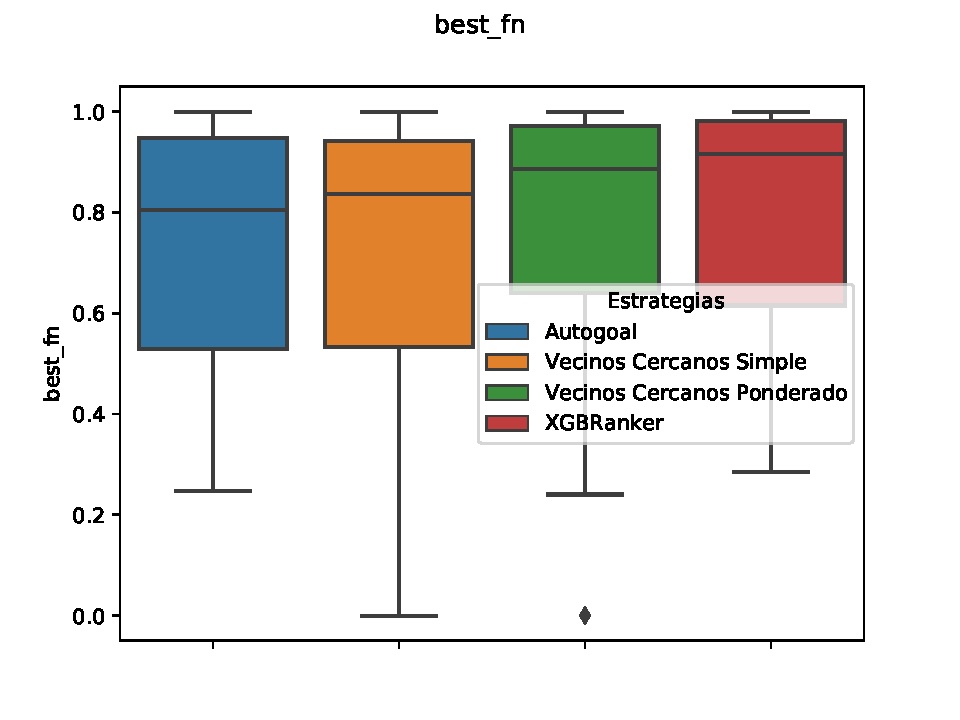
\includegraphics[scale=.8]{Figures/best-fn.pdf}
\caption{Mejor resultado de rendimiento obtenido en la búsqueda de los flujos de algoritmos en cada uno de los datasets de prueba para las diferentes estrategias.}
\label{fig:bestfn}
\end{figure}

La Figura~\ref{fig:zscore} muestran los resultados obtenidos estandarizados. Los valores atípicos fueron omitidos para un mejor análisis de la gráfica. Para su normalización, fue usada la Puntuación Z o \textit{Z-Score}, que se utiliza en estadística para comparar datos procedentes de diferentes muestras o poblaciones. Se define como el número de desviaciones típicas que un valor dado toma con respecto a la media de su muestra o población. Sea $x$ el mejor resultado alcanzado en un dataset, $\mu$ y $\sigma$ la media y la desviación estándar de los resultados obtenidos en ese dataset, el valor z de este dataset es: $$z = \dfrac{x - \mu}{\sigma}$$

Los resultados de la Figura~\ref{fig:zscore} muestran una pequeña mejora en la estrategia de Vecinos Cercanos Simple y XGBRanker con respecto a AutoGOAL, mientras que no se puede apreciar mucha diferencia con respecto a los resultados obtenidos utilizando el método de Vecinos Cercanos Ponderados. Sin embargo, es necesario tener en cuenta que esta métrica no fue la usada en el entrenamiento de los modelos de meta-learning. Las estrategias que usan directamente el resultado de rendimiento, y no este valor normalizado, como la de Vecinos Cercanos Ponderado y XGBRanker, pueden estar afectadas en la comparación con esta métrica. A pesar de esto, se puede concluir que los resultados alcanzados por AutoGOAL usando las estrategias de meta-learning superan aquellos obtenidos por AutoGOAL sin meta-learning.

\begin{figure}[H]
	\centering
	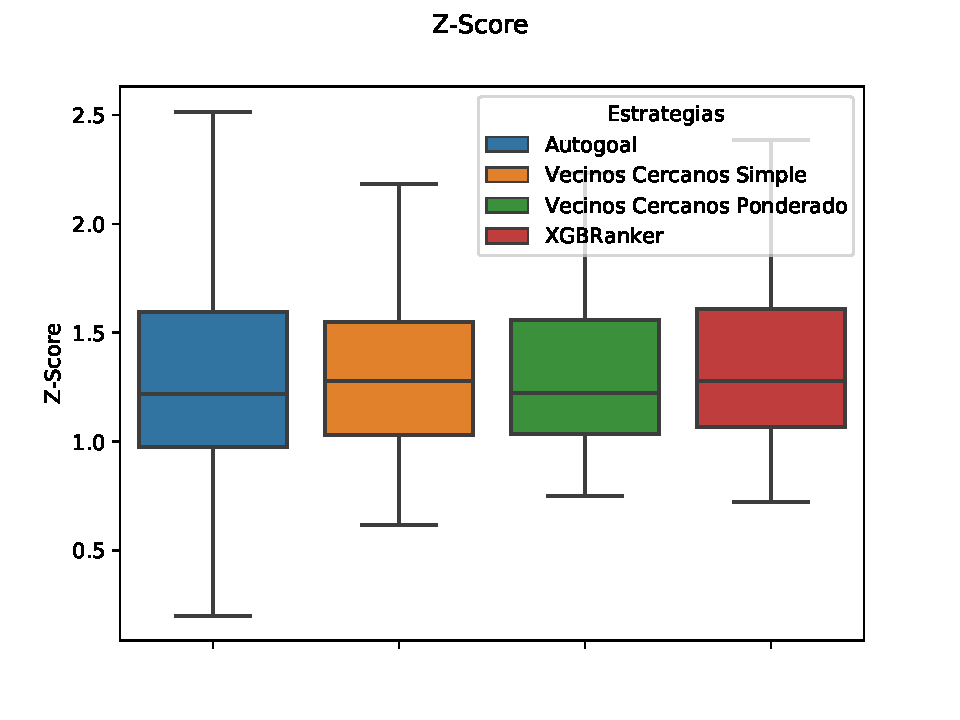
\includegraphics[scale=.8]{Figures/z-score.pdf}
	\caption{Puntuación Z obtenida en la búsqueda de los flujos de algoritmos en cada uno de los datasets de prueba para las diferentes estrategias.}
	\label{fig:zscore}
\end{figure}

Los resultados experimentales fueron implementados utilizando el mismo código en todos los experimentos. Para cada una de las variantes analizadas, los experimentos se ejecutan bajo la misma restricción de tiempo (30 minutos de ejecución total y 5 minutos de ejecución para un solo modelo), por lo tanto, cada una de las estrategias probadas tiene el mismo tiempo para la búsqueda de los flujos de algoritmos. Las experimentaciones realizadas muestran que el conocimiento adicional obtenido al principio mediante la técnica de meta-learning desarrollada cuando es agregado al proceso de optimización, obtiene resultados satisfactorios. En cuanto a la cantidad de flujos inválidos generados y la velocidad con la que se encuentra el mejor resultado de rendimiento, en promedio, los modelos que usan la técnica de meta-learning obtienen mejores resultados con respecto al modelo donde no se aplica.


% Falta hablar más de los resultados, sobre todo que quede claro la mejora o la diferencia...

\section{Discusión}\label{sec:discusion}

%- Hablar de la evidencia de que el sistema funciona 
%
%- Limitaciones:
%
%	+ Tener en cuenta métricas multi-objetivos
%	
%	+ Adaptarlo para usar regresión
%	
%	+ Hablar de las limitaciones de los datasets, de mayor variedad y de una mayor diversificación en sus características
%	
%	+ Hablar de los meta-features, del estudio la posible selección de estas


El método propuesto tiene también algunas limitaciones, las cuales se pueden mejorar en trabajos futuros. Con respecto a la métrica usada para determinar el rendimiento de cada flujo, se usa la métrica por defecto de AutoGOAL, \textit{accuracy}. Sin embargo, en escenarios prácticos, puede ser necesario equilibrar diferentes métricas de rendimiento, incluido también el uso del tiempo y la memoria, y cualidades más subjetivas como la interpretabilidad de los modelos o su capacidad para lidiar con datos sesgados. El enfoque de optimizar una métrica principal sujeta a restricciones de tiempo y memoria usada en AutoGOAL, y, por lo tanto, también en la propuesta diseñada, es insuficiente en un escenario en el que el usuario final tiene que decidir sobre cuestiones prácticas como el despliegue de estos flujos en un sistema de producción. % A modo de ejemplo, TPOT~\cite{olson2019tpot} considera este problema desde el enfoque multi-objetivo mediante la optimización conjunta de la precisión y la complejidad del modelo (en términos de longitud de los flujos). También se han implementado eficientemente medidas multi-criterio en sistemas de meta-learning~\cite{bradzil2003ranking}, donde se crea el ranking de algoritmos basado en \textit{accuracy} y tiempo, mediante la métrica denominada \textit{Adjusted Ratio of Ratios} (ARR)~\cite{soares2000measures}

La experimentación llevada a cabo se realizó solo con datasets de clasificación, por lo que solo se estudiaron los resultados obtenidos en esa tarea. Para demostrar la utilidad de la estrategia de meta-learning implementada en una gran gama de tareas es necesario la experimentación en diferentes tipos de tareas de aprendizaje, por ejemplo, de regresión.  Sin embargo, el modelo propuesto es adaptable a cualquier tipo de problema de aprendizaje automático siempre y cuando se tenga una medida para determinar la eficiencia de un flujo de algoritmos en un dataset. Para la realización de varios tipos de tareas, se propone la creación de un modelo diferente para cada tipo de problemas. Es decir, se crearía un modelo para las tareas de clasificación y otro para regresión. De esta manera, para el análisis de un dataset es necesario conocer el tipo de tarea que se quiere resolver, y usar el modelo adecuado para ella.

Meta-learning es muy dependiente de la calidad de los meta-ejemplos que usa para su entrenamiento~\cite{gomes2012combining}. Usualmente, es difícil obtener buenos resultados, ya que las meta-características son frecuentemente bastante ruidosas, porque el cálculo de estas está propenso a errores. Además, el número de problemas disponibles para la generación de meta-ejemplos generalmente es limitada. En este trabajo, se obtienen buenos resultados debido al uso de meta-características que han sido ampliamente utilizadas en la literatura y a la gran variedad de datasets extraídos. Sin embargo, se considera que un análisis más detallado de la distribución de los datasets para excluir aquellos que tienen características atípicas, y la inclusión de datasets de mayor tamaño puede proporcionar mejores resultados. De igual manera, un estudio de las meta-características para la eliminación de aquellas que proporcionen información poco útil debe proporcionar mejoras en el método propuesto. Además, el uso de la medida normalizada (\textit{z-score}) en el entrenamiento de las estrategias implementadas, puede proporcionar mejoras para la selección justa de flujos de algoritmos en distintos datasets.







\backmatter

\begin{conclusions}\label{conclusion}

\qquad 

%- Hablar de manera general del aumento del desarrollo en la ia
%- Hablar de las soluciones de AutoML, y luego de las soluciones de meta-learning
%- Hablar de lo que le faltan a las soluciones de meta-learning implementadas (como en las conclusiones de background)
%- Hablar luego de las características de la solución (como está en la introducción de propuesta)
%- Hablar de los resultados obtenidos en la experimentación

La inteligencia artificial, y en particular el aprendizaje automático, es cada vez más demandado en la industria, debido al potencial que tiene para automatizar los procesos más complejos. Las organizaciones están repletas de datos, pero carecen de personas con la experiencia técnica necesaria para transformar estos datos en conocimientos prácticos~\cite{miller2017quant}. Entre las principales dificultades para aplicar extensivamente técnicas de aprendizaje automático en problemas reales, están la poca disponibilidad de expertos unido al costo de diseñar, implementar y evaluar este tipo de soluciones. 

Con el objetivo de liberar a los expertos de las tareas menos creativas en la implementación de sistemas de aprendizaje automático, las organizaciones se están volcando cada vez más hacia la automatización en el trabajo de ciencia de datos, comenzando con la adopción de técnicas que automatizan la creación de modelos de aprendizaje automático~\cite{drozdal2020trust, wang2019humanai}. Sin embargo, la adopción de esta tecnología en entornos empresariales no ha sido perfecta. Actualmente, las herramientas de AutoML tienen restricciones respecto a lo que pueden realizar de manera flexible~\cite{crisan2021fits}. %Los sistemas de extremo a extremo que abarcan todo el espectro del trabajo de la ciencia de datos, desde la preparación de los datos hasta la comunicación, aún no se han realizado por completo~\cite{lee2019AHP, zoller2019surver}.

Una de las limitaciones presente en los primeros sistemas de AutoML consiste en su inhabilidad de rehusar conocimiento previo para solucionar nuevas tareas. Para cerrar esta brecha, las herramientas de AutoML comenzaron a aplicar técnicas de meta-learning, las cuales tienen el objetivo de obtener modelos para nuevas tareas usando experiencias previas. Este tipo de estrategias ayudan a disminuir el costo de aplicar AutoML, al relacionar un nuevo conjunto de datos con los mejores flujos obtenidos en problemas similares previamente resueltos. 

Aunque existen varias herramientas de meta-learning que han sido exitosas al aplicarse a AutoML, resolviendo problemas específicos de inteligencia artificial, estas herramientas son aún demasiado rígidas para ser utilizadas en problemas prácticos que requieren la combinación de algoritmos y tecnologías de diferente naturaleza. La propuesta de meta-learning implementada es capaz de abordar una gran variedad de problemas mediante la selección de meta-características capaces de representarlos. Además, explorando la interacción entre las características de los datasets y la estructura de los flujos, el método propuesto es capaz de identificar flujos con un buen rendimiento sin realizar un análisis computacionalmente costoso. Como sistema de AutoML complementario se eligió AutoGOAL, que destaca por su capacidad de generar soluciones eficaces para una amplia gama de tareas y dominios, permitiéndole resolver una amplia gama de tareas. AutoGOAL es usado para la generación de flujos de algoritmos para crear la base de conocimiento, por lo que se presenta gran diversidad en los flujos guardados debido a la variedad de herramientas de aprendizaje automático que AutoGOAL utiliza.

El enfoque desarrollado se propone como un paso preliminar para otras soluciones más costosas computacionalmente, como por ejemplo, para la inicialización de sistemas de AutoML. En esta investigación AutoGOAL también es usado como herramienta complementaria en el proceso de búsqueda de flujos. Por lo tanto, se describe como se realiza la adición de conocimiento experto a la estrategia de búsqueda utilizada por AutoGOAL: \textit{Probabilistic Grammatical Evolution}~\cite{pge2015}, que no había sido usada anteriormente con meta-learning.

Para la realización de la propuesta, se extrajeron meta-características, que, además de proveer información referente a los datos del dataset (relacionados a valores medios, desviación estándar, etc), son capaces de proporcionar conocimiento sobre la tarea que el dataset está representando. Además, mediante la extracción de flujos de aprendizaje a través de AutoGOAL, se obtuvo una gran variedad de flujos de algoritmos. Esto, junto con la gran cantidad de datasets utilizados garantiza la capacidad de abarcar una gran cantidad de tareas.

La propuesta de meta-learning consiste en la selección de un conjunto de flujos de algoritmos para ser propuestos en la inicialización de la optimización de AutoGOAL. La elección de este conjunto de flujos se realiza mediante un enfoque de ranking, en el que para un nuevo dataset se seleccionan los \texttt{k} mejores flujos de algoritmos. Para esto, se implementaron varias estrategias.

La evaluación experimental realizada en un gran número de datasets muestra que estas estrategias de meta-learning obtienen mejores resultados con respecto a AutoGOAL sin meta-learning, sin ninguna consideración de dominio o problema específico. Se tienen en cuenta varios factores: la cantidad de flujos inválidos generados por estas dos estrategias, la evolución del proceso de optimización a través de las iteraciones y los resultados de rendimiento obtenidos para cada una de las versiones probadas.

\section{Trabajos Futuros}

- Hablar de la necesidad de abarcar más tipos de problemas. 
- 

\end{conclusions}

\begin{recomendations}

El enfoque de meta-learning presentado en esta Tesis es utilizable en problemas prácticos y proporciona información importante en el proceso de AutoML, lo que le permite obtener mejores resultados en la búsqueda de flujos de algoritmos. Sin embargo, aún se encuentra en una etapa de desarrollo inicial, por lo que es necesario seguir mejorando sus capacidades mediante un estudio más exhaustivo.

El conocimiento obtenido con las distintas estrategias de meta-learning fue añadido a AutoML en el proceso de inicialización de la búsqueda de flujos de algoritmos. Sin embargo, existen distintas formas de añadir la experiencia previa obtenida mediante meta-learning al proceso de optimización. Algunas estrategias, como la desarrollada con el modelo de XGBoost puede ser utilizada como modelo sustituto que guíe el proceso de búsqueda de flujos. De esta forma, el conocimiento previo obtenido de experiencias pasadas será utilizable en la estrategia de búsqueda de flujos a lo largo del proceso de optimización.

Además, en la experimentación realizada en esta investigación se analizan los resultados obtenidos en el proceso de inicialización de AutoGOAL con un conjunto inicial de 15 flujos de algoritmos. El tamaño de este conjunto inicial, que es el usado para añadir conocimiento previo al proceso de AutoML, puede variar considerablemente el rendimiento final obtenido en la búsqueda de flujos~\cite{rankml}. Por lo tanto, se recomienda la realización de experimentos para encontrar el tamaño de ranking final óptimo para ser añadido como conjunto inicial a AutoML.

La generación de rankings en la estrategia de vecinos cercanos es otro de los aspectos que se puede estudiar más detalladamente. El método de generación de ranking mediante el mecanismo ponderado, en el que se tiene en cuenta la distancia entre el dataset a analizar y los datasets de la base de conocimiento y el valor del rendimiento de un flujo de algoritmos, puede ser mejorado. En la versión utilizada, se le da la misma importancia a ambos factores, evaluar el peso asignado a uno de los dos componentes puede hacer que mejoren los resultados obtenidos. De esta manera, para la generación de rankings, los resultados de rendimiento de los flujos de algoritmos pueden considerarse más importantes, priorizando este factor en el ranking resultante.


\end{recomendations}

%\bibliographystyle{babplain-uh}
%\bibliography{Bibliography}
\begin{thebibliography}{99}
	
\end{thebibliography}
%\bibliography{references}

\end{document}